\documentclass[a4paper,11pt,fleqn,twoside,openright]{memoir} 	% Openright aabner kapitler paa hoejresider (openany begge)

%%%% PACKAGES %%%%

% ¤¤ Oversaettelse og tegnsaetning ¤¤ %
\usepackage[utf8]{inputenc}					% Input-indkodning af tegnsaet (UTF8)
\usepackage[danish]{babel}					% Dokumentets sprog
\usepackage[T1]{fontenc}					% Output-indkodning af tegnsaet (T1)
\usepackage{ragged2e,anyfontsize}			% Justering af elementer
\usepackage{fixltx2e}						% Retter forskellige fejl i LaTeX-kernen
																			
% ¤¤ Figurer og tabeller (floats) ¤¤ %
\usepackage{graphicx} 						% Haandtering af eksterne billeder (JPG, PNG, PDF)
\usepackage{multirow}                		% Fletning af raekker og kolonner (\multicolumn og \multirow)
\usepackage{colortbl} 						% Farver i tabeller (fx \columncolor, \rowcolor og \cellcolor)
\usepackage[dvipsnames]{xcolor}				% Definer farver med \definecolor. Se mere: http://en.wikibooks.org/wiki/LaTeX/Colors
\usepackage{flafter}						% Soerger for at floats ikke optraeder i teksten foer deres reference
\let\newfloat\relax 						% Justering mellem float-pakken og memoir
\usepackage{float}							% Muliggoer eksakt placering af floats, f.eks. \begin{figure}[H]
%\usepackage{eso-pic}						% Tilfoej billedekommandoer paa hver side
%\usepackage{wrapfig}						% Indsaettelse af figurer omsvoebt af tekst. \begin{wrapfigure}{Placering}{Stoerrelse}
%\usepackage{multicol}         	        	% Muliggoer tekst i spalter
%\usepackage{rotating}						% Rotation af tekst med \begin{sideways}...\end{sideways}

%Plotting
\usepackage{siunitx}
\usepackage{tikz} % To generate the plot from csv
\usepackage{pgfplots}
\usepackage{filecontents}
\usetikzlibrary{datavisualization}
\usetikzlibrary{datavisualization.formats.functions}

\pgfplotsset{compat=newest} % Allows to place the legend below plot
\usepgfplotslibrary{units} % Allows to enter the units nicely

\sisetup{
  round-mode          = places,
  round-precision     = 2,
}




% ¤¤ Matematik mm. ¤¤
\usepackage{amsmath,amssymb,stmaryrd} 		% Avancerede matematik-udvidelser
\usepackage{mathtools}						% Andre matematik- og tegnudvidelser
\usepackage{textcomp}                 		% Symbol-udvidelser (f.eks. promille-tegn med \textperthousand )
\usepackage{siunitx}						% Flot og konsistent praesentation af tal og enheder med \si{enhed} og \SI{tal}{enhed}
\sisetup{output-decimal-marker = {,}}		% Opsaetning af \SI (DE for komma som decimalseparator) 
%\usepackage[version=3]{mhchem} 				% Kemi-pakke til flot og let notation af formler, f.eks. \ce{Fe2O3}
%\usepackage{rsphrase}						% Kemi-pakke til RS-saetninger, f.eks. \rsphrase{R1}

% ¤¤ Referencer og kilder ¤¤ %
\usepackage[danish]{varioref}				% Muliggoer bl.a. krydshenvisninger med sidetal (\vref)
\usepackage{natbib}							% Udvidelse med naturvidenskabelige citationsmodeller
%\usepackage{xr}							% Referencer til eksternt dokument med \externaldocument{<NAVN>}
%\usepackage{glossaries}					% Terminologi- eller symbolliste (se mere i Daleifs Latex-bog)

% ¤¤ Misc. ¤¤ %
\usepackage{listings}						% Placer kildekode i dokumentet med \begin{lstlisting}...\end{lstlisting}
\usepackage{lipsum}							% Dummy text \lipsum[..]
\usepackage[shortlabels]{enumitem}			% Muliggoer enkelt konfiguration af lister
\usepackage{pdfpages}						% Goer det muligt at inkludere pdf-dokumenter med kommandoen \includepdf[pages={x-y}]{fil.pdf}	
\pdfoptionpdfminorversion=6					% Muliggoer inkludering af pdf dokumenter, af version 1.6 og hoejere
\pretolerance=2500 							% Justering af afstand mellem ord (hoejt tal, mindre orddeling og mere luft mellem ord)

% Kommentarer og rettelser med \fxnote. Med 'final' i stedet for 'draft' udloeser hver note en error i den faerdige rapport.
\usepackage[footnote,final,danish,silent,nomargin]{fixme}		


%%%% CUSTOM SETTINGS %%%%

% ¤¤ Marginer ¤¤ %
\setlrmarginsandblock{3.5cm}{2.5cm}{*}		% \setlrmarginsandblock{Indbinding}{Kant}{Ratio}
\setulmarginsandblock{2.5cm}{3.0cm}{*}		% \setulmarginsandblock{Top}{Bund}{Ratio}
\checkandfixthelayout 						% Oversaetter vaerdier til brug for andre pakker

%	¤¤ Afsnitsformatering ¤¤ %
\setlength{\parindent}{0mm}           		% Stoerrelse af indryk
\setlength{\parskip}{4mm}          			% Afstand mellem afsnit ved brug af double Enter
\linespread{1,1}							% Linie afstand

% ¤¤ Litteraturlisten ¤¤ %
\bibpunct[,]{[}{]}{;}{a}{,}{,} 				% Definerer de 6 parametre ved Harvard henvisning (bl.a. parantestype og seperatortegn)
\bibliographystyle{bibtex/harvard}			% Udseende af litteraturlisten.

% ¤¤ Indholdsfortegnelse ¤¤ %
\setsecnumdepth{subsection}		 			% Dybden af nummerede overkrifter (part/chapter/section/subsection)
\maxsecnumdepth{subsection}					% Dokumentklassens graense for nummereringsdybde
\settocdepth{subsection} 					% Dybden af indholdsfortegnelsen

% ¤¤ Lister ¤¤ %
\setlist{
  topsep=0pt,								% Vertikal afstand mellem tekst og listen
  itemsep=-1ex,								% Vertikal afstand mellem items
} 

% ¤¤ Visuelle referencer ¤¤ %
\usepackage[colorlinks]{hyperref}			% Danner klikbare referencer (hyperlinks) i dokumentet.
\hypersetup{colorlinks = true,				% Opsaetning af farvede hyperlinks (interne links, citeringer og URL)
    linkcolor = black,
    citecolor = black,
    urlcolor = black
}

% ¤¤ Opsaetning af figur- og tabeltekst ¤¤ %
\captionnamefont{\small\bfseries\itshape}	% Opsaetning af tekstdelen ('Figur' eller 'Tabel')
\captiontitlefont{\small}					% Opsaetning af nummerering
\captiondelim{. }							% Seperator mellem nummerering og figurtekst
\hangcaption								% Venstrejusterer flere-liniers figurtekst under hinanden
\captionwidth{\linewidth}					% Bredden af figurteksten
\setlength{\belowcaptionskip}{0pt}			% Afstand under figurteksten
		
% ¤¤ Opsaetning af listings ¤¤ %
\definecolor{commentGreen}{RGB}{34,139,24}
\definecolor{stringPurple}{RGB}{208,76,239}

\lstset{language=Python,					% Sprog
	basicstyle=\ttfamily\scriptsize,		% Opsaetning af teksten
	keywords={for,if,while,else,elseif,		% Noegleord at fremhaeve
			  end,break,return,case,
			  switch,function},
	keywordstyle=\color{blue},				% Opsaetning af noegleord
	commentstyle=\color{commentGreen},		% Opsaetning af kommentarer
	stringstyle=\color{stringPurple},		% Opsaetning af strenge
	showstringspaces=false,					% Mellemrum i strenge enten vist eller blanke
	numbers=left, numberstyle=\tiny,		% Linjenumre
	extendedchars=true, 					% Tillader specielle karakterer
	columns=flexible,						% Kolonnejustering
	breaklines, breakatwhitespace=true,		% Bryd lange linjer
}

% ¤¤ Navngivning ¤¤ %
\addto\captionsdanish{
	\renewcommand\appendixname{Appendiks}
	\renewcommand\contentsname{Indholdsfortegnelse}	
	\renewcommand\appendixpagename{Appendiks}
	\renewcommand\appendixtocname{Appendiks}
	\renewcommand\cftchaptername{\chaptername~}				% Skriver "Kapitel" foran kapitlerne i indholdsfortegnelsen
	\renewcommand\cftappendixname{\appendixname~}			% Skriver "Appendiks" foran appendiks i indholdsfortegnelsen
}

% ¤¤ Kapiteludssende ¤¤ %
\definecolor{numbercolor}{gray}{0.7}		% Definerer en farve til brug til kapiteludseende
\newif\ifchapternonum

\makechapterstyle{jenor}{					% Definerer kapiteludseende frem til ...
  \renewcommand\beforechapskip{0pt}
  \renewcommand\printchaptername{}
  \renewcommand\printchapternum{}
  \renewcommand\printchapternonum{\chapternonumtrue}
  \renewcommand\chaptitlefont{\fontfamily{pbk}\fontseries{db}\fontshape{n}\fontsize{25}{35}\selectfont\raggedleft}
  \renewcommand\chapnumfont{\fontfamily{pbk}\fontseries{m}\fontshape{n}\fontsize{1in}{0in}\selectfont\color{numbercolor}}
  \renewcommand\printchaptertitle[1]{%
    \noindent
    \ifchapternonum
    \begin{tabularx}{\textwidth}{X}
    {\let\\\newline\chaptitlefont ##1\par} 
    \end{tabularx}
    \par\vskip-2.5mm\hrule
    \else
    \begin{tabularx}{\textwidth}{Xl}
    {\parbox[b]{\linewidth}{\chaptitlefont ##1}} & \raisebox{-15pt}{\chapnumfont \thechapter}
    \end{tabularx}
    \par\vskip2mm\hrule
    \fi
  }
}											% ... her

\chapterstyle{thatcher}						% Valg af kapiteludseende - Google 'memoir chapter styles' for alternativer

% ¤¤ Section style ¤¤ %

\usepackage{titlesec}
\titleformat{\section}
  {\normalfont\fontsize{14}{17}\scshape}{\thesection}{2em}{}


% ¤¤ Sidehoved ¤¤ %

\makepagestyle{Uni}							% Definerer sidehoved og sidefod udseende frem til ...
\makepsmarks{Uni}{%
	\createmark{chapter}{left}{shownumber}{}{. \ }
	\createmark{section}{right}{shownumber}{}{. \ }
	\createplainmark{toc}{both}{\contentsname}
	\createplainmark{lof}{both}{\listfigurename}
	\createplainmark{lot}{both}{\listtablename}
	\createplainmark{bib}{both}{\bibname}
	\createplainmark{index}{both}{\indexname}
	\createplainmark{glossary}{both}{\glossaryname}
}
\nouppercaseheads											% Ingen Caps oenskes

\makeevenhead{Uni}{Gruppe B205}{}{\leftmark}				% Definerer lige siders sidehoved (\makeevenhead{Navn}{Venstre}{Center}{Hoejre})
\makeoddhead{Uni}{\rightmark}{}{Aalborg Universitet}			% Definerer ulige siders sidehoved (\makeoddhead{Navn}{Venstre}{Center}{Hoejre})
\makeevenfoot{Uni}{\thepage}{}{}							% Definerer lige siders sidefod (\makeevenfoot{Navn}{Venstre}{Center}{Hoejre})
\makeoddfoot{Uni}{}{}{\thepage}								% Definerer ulige siders sidefod (\makeoddfoot{Navn}{Venstre}{Center}{Hoejre})
\makeheadrule{Uni}{\textwidth}{0.5pt}						% Tilfoejer en streg under sidehovedets indhold
\makefootrule{Uni}{\textwidth}{0.5pt}{1mm}					% Tilfoejer en streg under sidefodens indhold

\copypagestyle{Unichap}{Uni}								% Sidehoved for kapitelsider defineres som standardsider, men med blank sidehoved
\makeoddhead{Unichap}{}{}{}
\makeevenhead{Unichap}{}{}{}
\makeheadrule{Unichap}{\textwidth}{0pt}
\aliaspagestyle{chapter}{Unichap}							% Den ny style vaelges til at gaelde for chapters
															% ... her
															
\pagestyle{Uni}												% Valg af sidehoved og sidefod (benyt "plain" for ingen sidehoved/fod)


%%%% CUSTOM COMMANDS %%%%

% ¤¤ Billede hack ¤¤ %										% Indsaet figurer nemt med \figur{Stoerrelse}{Fil}{Figurtekst}{Label}
\newcommand{\figur}[4]{
		\begin{figure}[H] \centering
			\includegraphics[width=#1\textwidth]{billeder/#2}
			\caption{#3}\label{#4}
		\end{figure} 
}

% ¤¤ Specielle tegn ¤¤ %
\newcommand{\decC}{^{\circ}\text{C}}
\newcommand{\dec}{^{\circ}}
\newcommand{\m}{\cdot}


%%%% ORDDELING %%%%

\hyphenation{}											% Preamble indlaeses
\raggedbottom													% Soerger for at LaTeX ikke "straekker" teksten

%\includeonly{file1,file2}									% Inkluder kun specifikke filer (kommasepareret liste)

\begin{document}												% Starter dokumentet - obligatorisk

\frontmatter													% Forindhold - nummereres med romertal

\thispagestyle{empty}
\begin{flushright}
\vspace{3cm}

\phantom{hul}

\phantom{hul}

\phantom{hul}

\textsl{\Huge Lineær algebra i billedbehandling og -komprimering} \\


\rule{13cm}{3mm} \\ \vspace{1.5cm}
\vspace{1cm}
\centering

\includegraphics[width=0.7\textwidth]{Billeder/lenaQ5}

\vspace{2cm} 
\textsc{\Large P1 Projekt \\
Gruppe B205 \\
Matematik-Teknologi\\
Aalborg Universitet\\
Den 18. december 2015\\}
\end{flushright}

\cleardoublepage											% Indsaetter tom side, saa naeste kapitel starter paa hoejre side (hvis noedvendigt)
% Dette er LaTeX-versionen af titelbladet for TNB studenterrapporter
% Filen kræver:
% Universitetets logo:  AAU-logo-stud-UK eller AAU-logo-stud-DK
% Synopsis: En fil ved navn synopsis.tex


\phantomsection
\pdfbookmark[0]{Titelblad}{titelblad}
\thispagestyle{empty}

\begin{minipage}[t]{0.48\textwidth}
\vspace*{-25pt}			%\vspace*{-9pt}

\includegraphics[height=4cm]{billeder/AAU-logo-stud-DK-RGB}
\end{minipage}
\hfill
\begin{minipage}[t]{0.48\textwidth}
{\small 
\textbf{Første Studieår v/ Det Teknisk-}\\
\textbf{Naturvidenskabelige Fakultet}  \\
Matematik-Teknologi \\
Strandvejen 12-14 \\
9000 Aalborg \\
http://www.tnb.aau.dk}
\end{minipage}

\vspace*{1cm}

\begin{minipage}[t]{0.48\textwidth}
\textbf{Titel:} \\[5pt]\hspace*{2ex}
Lineær algebra i billedbehandling \\\hspace*{2ex}
og -komprimering \\\hspace*{2ex}



\textbf{Projekt:} \\[5pt]\bigskip\hspace{2ex}
P1-projekt

\textbf{Projektperiode:} \\[5pt]\bigskip\hspace{2ex}
September 2015 - December 2015

\textbf{Projektgruppe:} \\[5pt]\bigskip\hspace{2ex}
B205

\textbf{Deltagere:} \\[5pt]\hspace*{2ex}
Frederik A. Vardinghus-Nielsen \\\hspace*{2ex}
Mike L. H. Nguyen \\\hspace*{2ex}
Thomas Kjems \\\hspace*{2ex}
Sebastian E. Schrøder \\\hspace*{2ex}
Kenneth Borup \\\hspace*{2ex}

\textbf{Vejledere:} \\[5pt]\hspace*{2ex}
Christoffer Eg Sloth  \\\bigskip\hspace{2ex}
Mikkel Meyer Andersen

\vspace*{1cm}

\textbf{Oplagstal: 7} \\
\textbf{Sidetal: 79} \\
\textbf{Appendiks: 4} \\ 
\textbf{Afsluttet 18-12-2015}

\end{minipage}
\hfill
\begin{minipage}[t]{0.483\textwidth}
Synopsis: \\[5pt]
\fbox{\parbox{7cm}{\bigskipThis paper deals with the problem of ever growing resolutions, and therefore file sizes, of images taken with cameras on mobile phones. It examines two different signal processing techniques, which both detect correlation between values in an input signal, in the process of creating two different image compression algorithms. The two techniques are; a Discrete Cosine Transform and Principal Component Analysis. This paper will account for the mathematical properties of each of the techniques, incorporate them into image compression algorithms, and evaluate each algorithm by comparing quality and compression ratio of various test images for each algorithm. Through this comparison this paper determines which of the two is best suited as an image compression program for images taken with a mobile phone. This paper concludes, that the algorithm based on the Discrete Cosine Transform is more efficient at compressing images than the algorithm based on Principal Component Analysis, and it is therefore more suited as an image compression program for mobile phones.\bigskip}}
\end{minipage}

\vfill

{\footnotesize\itshape Rapportens indhold er frit tilgængeligt, men offentliggørelse (med kildeangivelse) må kun ske efter aftale med forfatterne.}

% Rapportens indhold er frit tilgængeligt, men offentliggørelse (med kildeangivelse) må kun ske efter aftale med forfatterne.
% The content of the report is freely available, but publication (with source reference) may only take place in agreement with the authors.

\cleardoublepage
\chapter*{Forord}
Følgende rapport er udarbejdet af 1. semester studerende på uddannelsen for Matematik-teknologi ved Aalborg Universitet. Det overordnede tema for projektet er \textit{Anvendt lineær algebra inden for teknologi}.

Rapporten omhandler projektkatalogets første projekt \textit{Billedekomprimering}, hvor der undersøges forskellige metoder/matematiske modeller til komprimering af et billede. Fokus lægges på komprimeringsmetoderne DCT (brugt i bl.a. JPEG-komprimering) og PCA.

Forudsætningerne for at læse rapporten er et vist kendskab til lineær algebra og opbygningen af digitale billeder og tilhørende data, såvel som en indsigt i hvad en digital komprimeringsmetode er og gør.\\

\textbf{Læsevejledning}\\
Igennem rapporten er der kildehenvisninger, som afslutningsvist er samlet i en kildeliste bagerst i rapporten. Disse er opsat efter Harvardmetoden, hvorved kilder i teksten refereres med [Efternavn, [År], Side/Afsnit/Tidsinterval] (dog refereres der kun til årstal, såfremt dette kendes og kun til sidetal/afsnit, hvor dette giver mening). Kilden henviser til kildelisten, hvor boglige kilder er angivet med forfatter, titel, udgave og forlag, mens hjemmesider er angivet med forfatter, titel og dato for besøg.
Figurer, tabeller og ligniger er nummereret i forhold til kapitel, hvorved eksempelvis første figur i kapitel 5 angives som \textit{Figur 5.1}, den næste figur hedder derved \textit{Figur 5.2} osv. Samme talnummerering findes på tabeller og lignigner, men kun tabeller og figurer har en forklarende tekst under de respektive figurer og tabeller. Talformateringen er dansk og decimalseperator er ","\phantom{i}og tusindseperator er ".".

Der er i løbet af rapporten refereret til komprimeringsprogrammer såvel som billeder. Disse er at finde på nedenstående link, hvor billederne også kan ses i fuld størrelse:\\
Bilagslink: \href{https://goo.gl/qpC2Kz}{www.goo.gl/qpC2Kz}\\
Indholdsfortegnelsen af dette link ses under appendiks \ref{dropbox}.


\phantom{Luft}

\phantom{Luft}

\begin{table}[H]
	\centering
		\begin{tabular}{ccc}
			\underline{\phantom{mmmmmmmmmmmmmm}} & \underline{\phantom{mmmmmmmmmmmmm}} & \underline{\phantom{mmmmmmmmmmmmm}} \\
			Frederik A. Vardinghus-Nielsen			& Mike L. H. Nguyen 		& Thomas Kjems 			\\
			&&\\
			&&\\
			\underline{\phantom{mmmmmmmmmmmmmm}} & \underline{\phantom{mmmmmmmmmmmmm}} \\
			Sebastian E. Schrøder			& Kenneth Borup 				\\
			&&\\
			&&\\
											
		\end{tabular}
\end{table}
\cleardoublepage

%%%% Indholdsfortegnelse (TOC) %%%%

\phantomsection													% Kunstigt afsnit, som hyperlinks kan 'holde fast i'
\pdfbookmark[0]{Indholdsfortegnelse}{indhold}						% Tildeler en klikbar bookmark til den endelige PDF
\tableofcontents*												% Indholdsfortegnelsen (kaldet ToC) 

%\addtocontents{toc}{\protect\newpage}							% Fremtvinger sideskift i ToC hvis noedvendig (der hvor koden placeres)


\mainmatter														% Hovedindhold - nummereres fra side 1

%%%% Rapportindhold %%%% 										% Rapportindholdet boer IKKE indeholde broedtekst - KUN includede filer!

%% Indledende %%												% Opdel evt. i passende afsnit for overblikkets skyld

%\chapter{Indledning}

Når man i dag skal sende et billede, eller lægge det over på sin computer og det fylder for meget, kan man bare tag det ind i et program som photoshop eller lignede og bede den om at komprimere billedet for dig, og man kan endda selv vælge hvilken kvalitet den skal komme ud i, så efter et par minutter kommer det samme bilede ud men det fylder mindre. procenssen bag billed komprimeringen er i store omfang lineær algebra, altså operationer på matricer. 

\chapter{Projektbeskrivelse}
Følgende afsnit har til formål at skabe rammerne for rapportens retning igennem en problemanalyse, problemformulering og et metodeafsnit. Problemanalysen analyserer det initierende problem og undersøger præmisserne for problemet. Dette bliver efterfølgende brugt til klarlægning af problemformuleringen, der har hovedfokus på billedkomprimeringsmetoder vha. lineær algebra.

\section{Problemanalyse}
Digitale billeder er en stor del af mange menneskers hverdag, både direkte og indirekte, og har ligeledes en afgørende betydning for mange store teknologivirksomheders eksistens. Qua den rivende hurtige teknologiudvikling det seneste årti, er kameraer i mobiltelefoner blevet udviklet til at have bl.a. højere opløsning. Højere opløsning betyder, at billedfilerne også fylder betydeligt mere digital hukommelse, hvorved en mobiltelefons lagerplads hurtigere end tidligere opfyldes. Det betyder ydermere, at download og upload til internettet bliver langsommere, da en større mængde data tager længere tid at downloade end en lille mængde data.

Den enkelte bruger, der typisk besidder et stort fotoalbum på sin mobil, påvirkes af den stigende størrelse på billedfilerne. Dette gør de ved, at deres mobiltelefons lagerplads hurtigere bliver opfyldt af billederne, og da de fleste ønsker at gemme så mange billeder som muligt, kan det være interessant at komprimere billederne for at få plads til flere billeder.

Hele essensen i komprimering af billeder er at gøre filerne mindre, hvorved de fylder mindre lagerplads, hvilket kan anses som en billedbehandling. Billedet, der behandles, kan anses som værende en $m \times n$ matrix, hvor $m$ og $n$ er billedets dimensioner i pixels. Indholdet i matricen er billedets pixelværdier, og indeholder forskellige data afhængigt af billedformatet. Billedbehandlinger, såsom komprimering, fremkommer ved operationer på matricen, og er af den matematiske gren lineær algebra, der netop omhandler matrixoperationer.

Der findes mange forskellige komprimeringsmetoder, og disse kan grundlæggende opdeles i to forskellige typer; tabsfri og ikke-tabsfri komprimering. Tabsfri komprimering er en komprimering af dataene uden at fjerne noget data, og ikke-tabsfri er det modsatte; en komprimering med tab af data.\\
JPEG-komprimering er den mest udbredte komprimeringsmetode, og har oprindelse i gruppen med samme initialer; Joint Photographic Experts Group. Metoden som bruges i JPEG er tilnærmelsesvist en \emph{Diskret Cosinus Transformation} (fremover kaldet DCT), som fungerer på baggrund af tesen om at menneskets syn ikke særlig godt ser høje frekvenser, hvorfor disse kan fjernes fra billedet uden betydelig synlig ændring. DCT er en ikke-tabsfri komprimeringsmetode og ved dekodning af den komprimerede fil, vil det genskabte billede kun være en tilnærmelse af det originale, og ikke en eksakt kopi. Forskellen mellem det genskabte og originale billede er de høje frekvenser, og tabet ved komprimeringen burde derfor ikke være synlig for det blotte øje. DCT er datauafhængig og transformationerne fungerer derved på alle billeder (dog med forskellig kvalitet).
En anden metode til komprimering er \emph{Principal Component Analysis} (fremover kaldet PCA), der ligesom DCT er en ikke-tabsfri komprimeringsmetode. PCA er en statistisk metode, der i store mængder data identificerer signifikante (og dermed også insignifikante) data. PCA finder kovariansen mellem dataene og tildeler de enkelte dimensioner en egenvektor med dertilhørende egenværdi, der bruges til vurdering af signifikante og insignifikante data. Akserne med størst varians udtrykker mest af billedet, og akserne med mindst varians fjernes derfor i komprimeringen. Modsat DCT fjernes de høje frekvenser ikke med PCA, men derimod de data der har mindst betydning for billedets repræsentation. Det betyder dog også at billedet (ligesom DCT) blot skaber en tilnærmelse af det oprindelige billede ved dekodning. PCA er dataafhængig, og billedet har større betydning for komprimeringen med PCA end med DCT.

På trods af mange ligheder mellem PCA og DCT, fungerer de i praksis meget forskelligt, hvilket også betyder at de har hver deres fordele og ulemper. Det betyder også at hver metode fungerer bedre på nogle former for billeder end andre, hvorved det kan være svært at finde den bedst egnede metode til et vilkårligt billede.

\subsection*{Hastighed}
I forbindelse med brug af et komprimeringsprogram i dagligdagen er det afgørende, at tiden det tager at udføre komprimeringen, er så kort som mulig, da det må antages at de fleste ønsker, at komprimeringen skal foregå hurtigst muligt. Da projektet ikke har sin kerne i programmering og kvaliteten af de programmer, der er udviklet til komprimeringen, er fokus ikke lagt på dette. Det betyder imidlertid, at hastigheden ikke kan måles i programmerne, der er udviklet til dette projekt. Til gengæld kunne en kompleksitetsanalyse laves, som giver et udtryk for hvor mange beregninger, der skal laves for at lave de to komprimeringsmetoder. Kompleksitetsanalyse ser bort fra den respektive enhed, der laver beregningerne, og giver derfor et udtryk for antal beregninger, der skal laves. Kompleksitetsanalyse er dog også udenfor denne rapports fokusområde og udføres derfor ikke. Bemærk at hastigheden ved komprimering har stor betyding for metodens relevans i virkeligheden men undersøges ikke i denne rapport.

\section*{Case - billeder på mobiltelefoner}
Den følgende rapport har udgangspunkt i den stigende brug af mobiltelefoner som kamera i dagligdagssituationer, hvorved mængden af billeder på den gængse mobiltelefon stiger. Dette giver dog problemer med hurtigt fyldt lagerplads på mobiltelefonerne, og deraf frustrerede brugere. Ved at komprimere billederne opnås der mere fri hukommelse og dermed plads til flere billeder. Der er dog begrænsninger i forhold til kvaliteten af komprimeringen, da den hurtige teknologiudvikling også resulterer i større krav til billederne, der tages. Det er for brugeren vigtigt, at komprimeringen kan være en dagligdagsopgave, og dermed ikke kræver lang tid at udføre. Det er også vigtigt, at billederne bibeholder en vis skarphed og sin farve, for at brugeroplevelsen bibeholdes.

\section{Problemformulering}
I kommende rapport bliver digitale billeder komprimeret vha. lineær algebra og undersøges ud fra problemformuleringen: \\
\begin{itemize}
\item[] \textit{Hvilken af komprimeringsmetoderne DCT og PCA komprimerer bedst billedet Lena \citep{lena}, og hvordan fungerer disse komprimeringsmetoder rent matematisk?} \\
\item[] \textit{Hvilken af metoderne bibeholder bedst kvaliteten af billedet i forhold til komprimeringsgraden?} \\
\item[] \textit{Hvilken metode komprimerer bedst rigtige mobilbilleder, og er der nogen sammenhæng mellem disse resultater?}
\end{itemize}

\section*{Metode}
På trods af at der findes et utal af komprimeringsmetoder, undersøges der i følgende rapport blot komprimeringsmetoderne DCT og PCA. Begge metoder fungerer ved at fjerne de visuelt mindst relevante data om billedet. Komprimeringsmetodernes matematiske grundlag undersøges og bruges efterfølgende til udvikling af python-programmer til komprimering af et billede. Billedet der komprimeres er Lena \citep{lena}, som er $512 \times 512$ pixels stort og i farveformatet RGB (Rød, Grøn, Blå). Resultaterne af komprimeringerne bliver sammenlignet i forhold til parametrene komprimeringsgrad og billedekvalitet. Komprimeringsgraden bliver sammenlignet på baggrund af antal bits i det oprindelige billede i forhold til det komprimerede billede. Billedkvaliteten vurderes på baggrund af forskellene i pixelværdierne mellem det oprindelige og komprimerede billede såvel som ved SNR-værdien for de forskellige komprimeringsgrader. Afslutningsvist bruges komprimeringsprogrammerne på flere forskellige mobilbilleder, for at afklare hvilke parametre, der har betydning for hvilken af metoderne, der fungerer bedst ved dagligdagsbilleder taget med en mobil.

På baggrund af de ovenstående afsnit og dertilhørende data bliver der i afsnit \ref{sec:vurdering} vurderet på kvaliteten og komprimeringsgraden for de to metoder, og sætte dem i relation til casen for rapporten.

%% Teori introduktion %%

\chapter{Digitale billeder} \label{sec:teori_intro}
Digitale billeder består af pixels. En pixel er den mindste bestanddel i et digitalt billede og er små ensfarvede områder. I gråtonebilleder beskrives en pixels farveintensitet med en værdi fra nul til 255, hvor nul er sort, og 255 er hvid. Dette er de to ekstremer i gråtonerne - imellem de to er der yderligere 254 gråtoner, som udgør en glat overgang fra sort til hvid. Et gråtonebillede udgøres altså af pixels af op til 256 forskellige gråtoner.

Et farvebillede behøver flere værdier for at beskrive hver enkelt pixels farve. Der findes flere forskelllige farvemodeller til beskrivelse af farver. RGB-modellen (Rød, Grøn, Blå) er en udbredt additiv model, som beskriver en pixels farve med tre værdier; én for hver farves intensitet i den pågældende pixel, således: Pixel = $(R,G,B)$. RGB-modellen bruges digitalt til at vise farver på skærme. Modellen er en additiv model, da den adderer grundfarverne i modellen i skabelsen af nye farver. Adderes alle tre grundfarver med fuld intensitet fås hvid. Hvis sort ønskes bruges ingen farver. I skærme skabes oplevelsen af at se farver ved at flere grønne, røde eller blå pixels lyser, og da disse pixels er for små til at blive skelnet mellem af det menneskelige øje, opleves det som en kombination af disse - de adderes sammen til en ny farve [\citet{curtis_newbold}, afsnit 1-2]. På figur \vref{fig:RGB_pixels} ses hvordan flere forskelligfarvede pixels skaber et farveindtryk ud fra RGB-modellen. Digitale billeder er typisk defineret ud fra RGB, men i forbindelse med komprimering bruges farvemodellen YCbCR også ofte.
\begin{figure}[htbp]
\centering
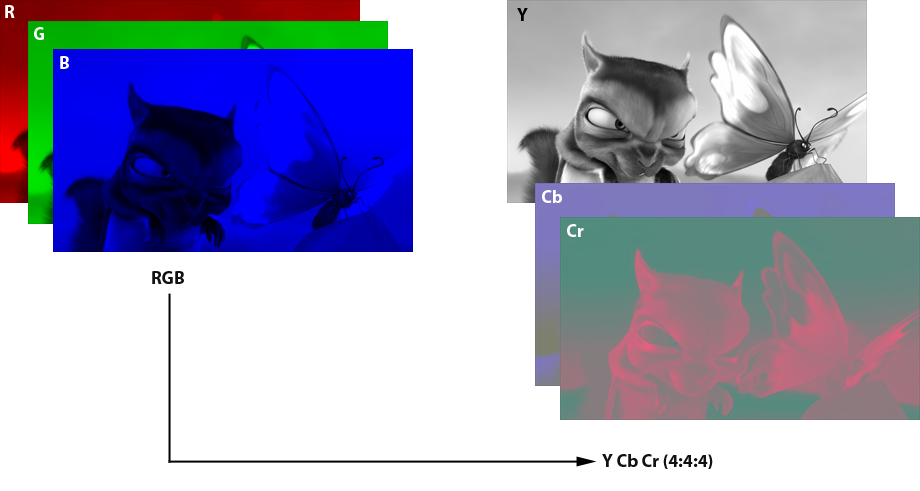
\includegraphics[width=0.75\textwidth]{Billeder/farvemodeller.png}
\caption{Eksempel på farvetransformation fra RGB til YCbCr [\citet{farvetransformation}, afsnit 4]}
\label{fig:farvemodeller}
\end{figure}
YCbCr står for \emph{Y}: Lysintensitet (en repræsentation af lysintensiteten i billedet), \emph{Cb} og \emph{Cr}: De to farverepræsentationer (hhv. blå minus \emph{Y} og rød minus \emph{Y}) [\citet{ycbcr_definition}, afsnit 1]. Fordelen ved YCbCr er at menneskets øje ikke opfatter forskelle i farver ligeså tydeligt som i lysintensitet, hvorved de to farverepræsentationer i højere grad kan komprimeres end lysintensiteten. Dette betyder at et billede i YCbCr-farverummet kan komprimeres mere end et i RGB-farverummet. Det skal dog bemærkes, at de to farverum udtrykker de samme data, blot med to forskellige baser. [\citet{ycbcr}, afsnit 2].

Der undersøges i følgende rapport med udgangspunkt i RGB-farverummet, da dette sparer transformationen til det nye farverum. Der ses bort fra, at brugen af YCbCr formentlig kunne have komprimeret billederne yderligere, men da forskelle på farverum ikke er fokus i denne rapport, bibeholdes billederne blot i RGB.
\begin{figure}[htbp]
\centering

\includegraphics[width=0.35\textwidth]{Billeder/RGB_pixels.jpg}
\caption{Nærbillede af pixels, i farverne RGB.}
\label{fig:RGB_pixels}
\end{figure}

Når hver pixel kan beskrives ved én eller flere værdier, kan det digitale billede repræsenteres fuldstændigt som en matrix med indgange for hver pixels farveintensitet. Hvis billedet er et digitalt billede af dimensionerne $m \times n$, kan det altså beskrives ved en $m \times n$ matrix. Undersøges farvebilleder, transformeres de enkelte farver hver for sig. Et eksempel på et gråtonebillede ses på figur \vref{eq:pixelmatrix}.

\begin{figure}[htbp]
\begin{minipage}[b]{0.25\linewidth}
\centering

\includegraphics[width=\textwidth]{Billeder/8x8_blok2.png}
\caption{Billede af $8\times8$ pixels.}
\label{fig:pixelblok}
\end{minipage}
\hspace{0.5cm}
\begin{minipage}[b]{0.5\linewidth}
\centering
\[\begin{bmatrix}
5	&	176	&	193	&	168	&	168	&	170	&	167	&	165\\
6	&	176	&	158	&	172	&	162	&	177	&	168	&	151\\
5	&	167	&	172	&	232	&	158	&	61	&	145	&	214\\
33	&	179	&	169	&	174	&	5	&	5	&	135	&	178\\
8	&	104	&	180	&	178	&	172	&	197	&	188	&	169\\
63	&	5	&	102	&	101	&	160	&	142	&	133	&	139\\
51	&	47	&	63	&	5	&	180	&	191	&	165	&	5\\
49	&	53	&	43	&	5	&	184	&	170	&	168	&	74
\end{bmatrix}
\]
\caption{$8\times8$ matrix for billedet.}
\label{eq:pixelmatrix}
\end{minipage}
\end{figure}
Når digitale billeder kan repræsenteres af matricer, betyder det også, at de kan behandles ved brug af regneregler for matricer. Moderne billedbehandlingsteknikker udnytter regneregler for matricer, altså lineær algebra til at behandle digitale billeder.

Ud over at være i stand til at blive behandlet vha. lineær algebra har billeder den egenskab, at nærliggende pixels i et billede ofte udviser stor korrelation - de ligner hinanden og pixels kan derfor ofte beskrives ud fra de nærliggende pixels [\citet{lokminglui_DCT}, s. 4]. Dette udnyttes i den senere billedkomprimering.

\section{Billedkomprimering}
Billedkomprimering er en billedbehandlingsteknik, som søger at komprimere en billedfils størrelse. Billedkomprimeringsmetoder kan opdeles i to kategorier; \emph{tabsfri} og \emph{ikke-tabsfri} komprimering.

Mængden hvorved et billede kan komprimeres afhænger af mange faktorer, som bl.a. inkluderer billedets størrelse, om det er i gråtoner, sort/hvid eller farver, hvor mange forskellige farveintensiteter billedet indeholder, og hvilket format billedet er i. Som følge af disse faktorer er det ikke altid muligt at udvikle den ideelle metode, som kun fjerner ubetydelig information - nogle gange er det nødvendigt også at fjerne betydningsfuldt information.\\
Tabsfri betegner en komprimeringsteknik, som under komprimeringen ikke forårsager noget tab af information fra det originale billede. Her udnyttes det, at inputtet af informationer ikke er homogent, og at der derfor kan laves en statistisk model over disse informationer. Modellen bruges til at lave en komprimering eksempelvis ved brug af entropikodning, som vil blive forklaret nærmere i afsnit \vref{sec:Huffman}. Ved brug af tabsfri komprimering, er det dekomprimerede billede magen til det originale. Som følge af bevaringen af alle informationer af det originale billede, er det ikke altid muligt at lave effektive komprimeringer. Blandt tabsfri billedformater kan nævnes PNG og TIFF. Essensen i disse metoder er at de finder fordelagtige måder at udtrykke de samme data på.

Ikke-tabsfri komprimering betegner en komprimeringsteknik, som under komprimeringen forårsager uigenkaldeligt tab af informationer om det originale billede. Det dekomprimerede billede er en efterligning af det originale billede. Det er ikke helt magen til da informationerne, som er brugt til dekomprimering, ikke er identiske med informationerne om det originale billede. Komprimeringsteknikker med tab benytter det faktum, at nogle af informationerne om billedet er visuelt ligegyldige for det menneskelige øje. Som følge af dette kan et billedets kvalitet byttes for højere komprimeringsgrad, hvorved en større del betydelige informationer om det origninale billede tabes. Som følge af denne komprimeringstekniks større råderum i forhold til den tabsfri, kan denne også opnå langt større komprimeringsgrader end den tabsfri. Blandt billedformater med tab kan nævnes GIF og PNG [\citet{matthews}, afsnit 2 og 4].

Det udnyttes ofte i ikke-tabsfri komprimering, at nærliggende pixels i et billede har stor korrelation og derfor til en vis grad kan udtrykkes ved én samlet værdi i stedet for en værdi for hver enkelt pixel. Til dette bruges en transformation, som kan transformere et input med stor korrelation til et output uden stor korrelation, men som udtrykker korrelationen i det originale input [\citet{lokminglui_DCT}, s. 2 og 4]. I domænet med de ukorrellerede koefficienter, kan der derefter sorteres i koefficienterne for at bevare de, som er vigtigst for det samlede udtryk i det orginale input.

%% DCT %%

\chapter{Billedkomprimering med diskret cosinustransformation} \label{chapter:DCT}
I dette kapitel udarbejde en billedkomprimeringsalgoritme med tab med udgangspunkt i den
en diskret cosinustransformation. Før denne forklares, er det nødvendigt at undersøge
den diskrete Fouriertransformation, som den stammer fra.
\section{Diskret Fouriertransformation}
Inden for signalbehandling er den Diskrete Fouriertransformation (DFT) et kendt værktøj. Transformationen er en lineær transformation, som udtrykker et signal på bølgeform ved sinus- og cosinusfunktioner [\citet{thefouriertransform}, afsnit 1]. De fleste signaler er på bølgeform og kan derfor beskrives ved sinus- og cosinusfunktioner gennem DFT.\\
Signalerne kan beskrives i to domæner
\begin{itemize}
\item \textit{Tidsdomænet}\\
		Signalet beskrives ved funktionsværdier til tiden $t$, $f(t)$.
\item \textit{Frekvensdomænet}\\
		Signalet beskrives ved amplitude og fase for en frekvensfunktion.
\end{itemize}
Regneoperationer i tidsdomænet har tilsvarende regneoperationer i frekvensdomænet, som ofte er beregningsmæssigt simplere [\citet{nbtwiki}, afsnit 2]. Af denne grund bruges den diskrete Fouriertransformation til signalbehandling.\\
Transformationen har desuden den egenskab, at den energikomprimerer signalet, som behandles. Energikomprimering betegner en transformations evne til at udtrykke mange signalværdier med høje korrelationer i domænet som færre koefficienter med lav korrelation i kodomænet [\citet{smcnus_energy}, s. 1]. Koefficienterne i frekvensdomænet fortæller i hvor høj grad de enkelte basisfunktioner er repræsenteret i tidsdomænet - høje koefficienter viser en høj optræden af den tilhørende basisfunktion, mens lave koefficienter viser en lav optræden af den tilhørende basisfunktion.

Når DFT udtrykker korrelerede signalværdier som ukorrelerede koefficienter i frekvensdomænet, betyder det også, at transformationen ikke formår at lave energikomprimering i høj grad, hvis signalværdierne er ukorrelerede. Dette betyder at, hvis der ønskes høj energikomprimering, skal DFT kun bruges på signaler, som består af korrelerede værdier.

I billedkomprimering er det, som tidligere beskrevet, interessant at udtrykke et billede ved færre værdier, da der derfor er færre værdier at gemme. DFT kan være et værktøj til dette. Et billede  består netop af korrelerede værdier og DFT kan derfor bruges.

Det viser sig imidlertid, at der findes et bedre værktøj til transformation af korrelerede signalværdier til ukorrelerede koefficienter. Transformationen kaldes den diskrete cosinustransformation (DCT), og er udledt fra DFT [\citet{dft_argument}, s. 3]. Udledningen ses i appendiks \vref{DCT_udledning}.\\
DCT udmærker sig inden for billedbehandling på flere områder i forhold til DFT:
\begin{enumerate}
\item \textit{Energikomprimering}\\
	DCT opnår højere energikomprimering end DFT [\citet{smcnus_energy}, s. 3 og 5]. Den formår at udtrykke informationer om signalværdier i tidsdomænet som færre koefficienter i frekvensdomænet end DFT formår. Det er ønskværdigt at udtrykke mange informationer ved få koefficienter i billedkomprimering.
\item \textit{Reelle tal}\\
	DCT benytter sig udelukkende af reelle tal i de transformerede koefficienter, hvorimod DFT benytter sig af både reelle og komplekse tal som koefficienter. Det er ønskværdigt, at regne udelukkende med reelle tal, da dette forsimpler den videre behandling af signalet.
\end{enumerate}
Der findes desuden en transformation, som bygger på sinusfunktioner - den diskrete sinustransformation (DST). Denne transformerer også signalværdier om til frekvenskoefficienter, men energikomprimerer ikke godt - den er ringere end både DFT og DCT [\citet{smcnus_energy}, s. 5].

Som følge af ovenstående grunde er der valgt at bruge DCT i den mest udbredte open-source komprimeringsstandard; JPEG.\\
På baggrund af at DCT
\begin{itemize}
\item[-] har bedre energikomprimering end DFT [\citet{smcnus_energy}, s. 5], og dermed skal færre koefficienter end DFT bruges til at danne en god approksimation af et signal [\citet{dft_argument}, s. 5]
\item[-] ofte bruges i billedbehandling [\citet{DTT}, s. 1]
\item[-] bruges i JPEG [\citet{dft_argument}, s. 1]
\end{itemize}
tages der i denne opgave udgangspunkt i DCT til at udføre billedkomprimeringer.
\subsection{JPEG}
Joint Photographic Experts Group udgav i 1992 den første JPEG-standard, som komprimerede og dekomprimerede billeder efter en bestemt algoritme. Et program, som kan gøre dette, kaldes en codec. Standarden er open source, og er siden 1992 blevet forbedret flere gange. I denne rapport undersøges en simpel og tidlig version.\\
JPEG gør brug af fire skridt i sin algoritme for at komprimere et billede fra dets fulde størrelse til en fil af mindre størrelse. Den inverse algoritme bruges til at dekomprimere en JPEG-fil til et billede. Da JPEG er en ikke-tabsfri komprimeringsalgoritme, er det dekomprimerede billede kun en efterligning af det originale. [\citet{whydomath_basic}, afsnit 1-7].\\
De fire skridt, som forklares nærmere i et senere afsnit, ser ud som følgende
\begin{enumerate}
\item \textit{Forbehandling af billede}\\
	Forbehandlingen indebærer at dele billedet op i kvadratiske undermatricer af 64 pixels. Dette gøres for at gøre den videre behandling af billedet med den diskrete cosinustransformation mere effektiv. Derudover trækkes 128 fra hver indgang i hver undermatrix for at centrere undermatricerne omkring nul.
\item \textit{Diskret cosinustransformation}\\
	Den diskrete cosinustransformation energikomprimerer billedet ved at udtrykke korrelerede signalværdier som dekorrelerede koefficienter i frekvensdomænet.
\item \textit{Kvantisering}\\
	Kvantiseringen fjerner mindre vigtige informationer om billedet ved at fjerne de dekorrelerede koefficienter, som ikke er vigtige i forhold til de korrelerede signalværdier. Dette skridt gør algoritmen ikke-tabsfri.
\item \textit{Entropikodning}\\
	Entropikodningen opstiller en statistisk model over de kvantiserede koefficienter og koder dem i strenge bestående af 0 og 1, som kan gemmes effektivt i en fil, som er mindre end den oprindelige billedfil.
\end{enumerate}
For at forstå hvorfor og hvordan algoritmen virker er det nødvendigt først at forstå den diskrete cosinustransformation. Derfor bliver dette skridt forklaret først.
\subsection{Diskret Cosinustransformation}\label{sec:DCT}
En diskret cosinustransformation er en lineær transformation, som afbilder en $n$-dimensionel vektor fra domænet $\mathbb{R}^n$ til kodomænet $\mathbb{R}^n$ - altså har transformationen samme kodomæne som domæne. Basisvektorerne i transformationen udledes fra cosinusfunktioner med forskellige frekvenser. Som følge af dette bliver den $n$-dimensionelle vektor afbildet ind i frekvensdomænet - den udtrykkes som en sum af cosinusfunktioner med forskellige frekvenser. Et eksempel på en funktion udtrykt ved bølgefunktioner ses i figur \vref{fig:frequencydomain}.

Som tidligere nævnt er den diskrete cosinustransformation udledt fra den diskrete Fouriertransformation. Udledningen ses i appendiks \vref{DCT_udledning}.

DCT bruges i udstrakt grad i signalbehandling på grund af dens høje energikomprimering. DCT kan altså komprimere meget signalværdi ned til få værdier i frekvensdomænet og dermed udtrykke signalværdier med stor korrelation som koeffiencienter med lav eller ingen korrelation [\citet{lokminglui_DCT}, s. 1]. Transformationen fungerer dog bedst, når signalværdierne som transformeres, har en vis korrelation - hvis dette ikke er tilfældet, vil der ikke blive opnået gode resultater med transformationen.

DCT er imidlertid ikke den eneste transformation, som kan dekorrelere signalværdier. En anden kendt transformation er Karhunen-Loève transformationen. Denne transformation transformerer som cosinustransformationen også korrelerede koefficienter til dekorrelerede koefficienter. Karhunen-Loeve udmærker sig ved at tilpasse sig hvordan signalet ser ud, for således at kunne energikomprimere meget effektivt - transformationen afhænger altså af signalet. Dette gør transformationen i stand til at lave den mest effektive energikomprimering [\citet{lokminglui_DCT}, s. 15]. Det er imidlertid ikke tidsmæssigt effektivt at komponere en ny transformation, hver gang et nyt signal behandles og derfor bruges den diskrete cosinustransformation i JPEG. Denne har en algoritme, som genererer en generel transformation, der kan bruges på mange datasæt [\citet{electronic_engineering}, s. 2].

Da DCT er en lineær transformation, kan den bruges i billedbehandling til at energikomprimere digitale billeder, som har stor korrelation mellem nærliggende pixels.\\
\begin{figure}[htbp]
\centering
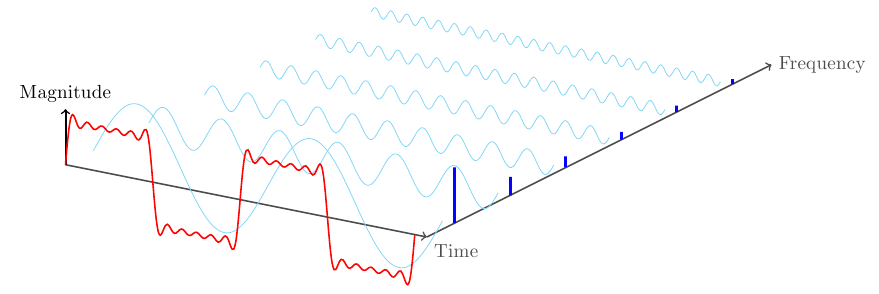
\includegraphics[width=0.7\textwidth]{Billeder/frequencydomain.png}
\caption{Signal (rød) og cosinusbølger (blå kurver) samt amplituden (søjler)[\citet{frequency_image}, \textit{Update 1}].}
\label{fig:frequencydomain}
\end{figure}
Den diskrete cosinustransformation, som kan udledes fra den diskrete Fouriertransformation, kan transformere i både én og to dimensioner. I denne opgave benyttes den todimensionelle. I ligning \vref{eq:DCTeq} ses den todimensionelle $n$-punkt diskrete cosinustransformation, hvor $T:\mathbb{R}^n \longrightarrow \mathbb{R}^n$ transformerer til en matrix indeholdende dekorrelerede koeffecienter. Matricen der transformeres, vil fremover refereres til som $A$. 
\begin{equation}
T_{(i,\ j)}=\sum\limits_{x=0}^{n-1} \sum\limits_{y=0}^{n-1} f(x,\ y) \cdot \alpha(i) \cdot \alpha(j) \cdot \cos\left(\frac{(2x+1) \cdot i \cdot \pi}{2n}\right) \cdot \cos\left(\frac{(2y+1) \cdot j \cdot \pi}{2n}\right)
\label{eq:DCTeq}
\end{equation} [\citet{guillermo_sapiro}, 7:12-11:10]\\
Hvor
\begin{itemize}
\item $T_{(i,\ j)}:$ indgang $(i,\ j)$ i den transformerede matrix ved DCT
\item $f(x,\ y):$ indgang $(x,\ y)$ i A
\item $n:$ matricens dimension
\item $\alpha(i)=\alpha(j)= \begin{cases}
					\sqrt{\frac{1}{n}} \ hvis \ i = 0\\
					\sqrt{\frac{2}{n}} \ hvis \ i \neq 0
					\end{cases}$
\end{itemize}
Det er værd at bemærke, at indgangene i matricen går fra $(0,\ 0)$ til $(n-1,\ n-1)$ i en $n \times n$ matrix. Ydermere er $\alpha(i)$  og $\alpha(j)$ normaliseringsfaktorer [\citet{normalization}, s. 96].

Ligning \ref{eq:DCTeq} bruges i denne opgave ikke til at beregne de transformerede koefficienter, da det beregningsmæssigt ikke er effektivt. Til dette bruges i stedet cosinustransformationen på matrixform, hvilket uddybes senere i dette afsnit. Ligning \ref{eq:DCTeq} er imidlertid god til at illustrere princippet bag transformationen, da det er tydeligt, hvordan cosinusfunktioner indgår i transformationen. Dette undersøges nu.

Det ses af ligning \vref{eq:DCTeq}, at hver transformeret indgang er summen af produktet af de 64 indgange i $A$ og en koefficient fra en cosinusfunktion. For hver række $f(x,\ y)$ holdes $x$ konstant gennem de otte søjler, hvor $y$ går fra $0-7$. Dette giver koefficienter, der alle ligger på en cosinuskurve. Hver gang en ny række $x$ påbegyndes, ændres amplituden af cosinusbølgen, som koefficienterne ligger på. Når en ny transformeret indgang $T_{(i,\ j)}$ beregnes, ændres $i$ og/eller $j$, og frekvensen af cosinusfunktionerne i transformen bliver højere. Altså bliver hver transformeret indgang et unikt aftryk af forskelligt svingene cosinusfunktioner og værdierne i matricen til billedet $A$.

For at illustrere princippet bag de skiftende amplituder og frekvenser af cosinusbølgerne som koefficienterne ligger på, er et sæt af to grafer for cosinustransformationen illustreret i figurerne \ref{fig:frekeksu1v1} og \ref{fig:frekeksu1v2}. Disse er tegnet ved brug af transformationen i ligning \vref{eq:DCTeq} for henholdsvis $T(1,\ 1)$ og $T(1,\ 2)$ og for $n=8$. For hver af funktionerne fremkommer otte bølger, og på hver af disse ligger de otte koefficienter ligeligt fordelt. På figur \ref{fig:cosko} ses de otte punkter på én af bølgerne for $T(0,\ 0)$ [\citet{whydomath_dct}, afsnit 3].

\begin{figure}[!h]
\begin{minipage}[b]{0.5\linewidth}
\centering
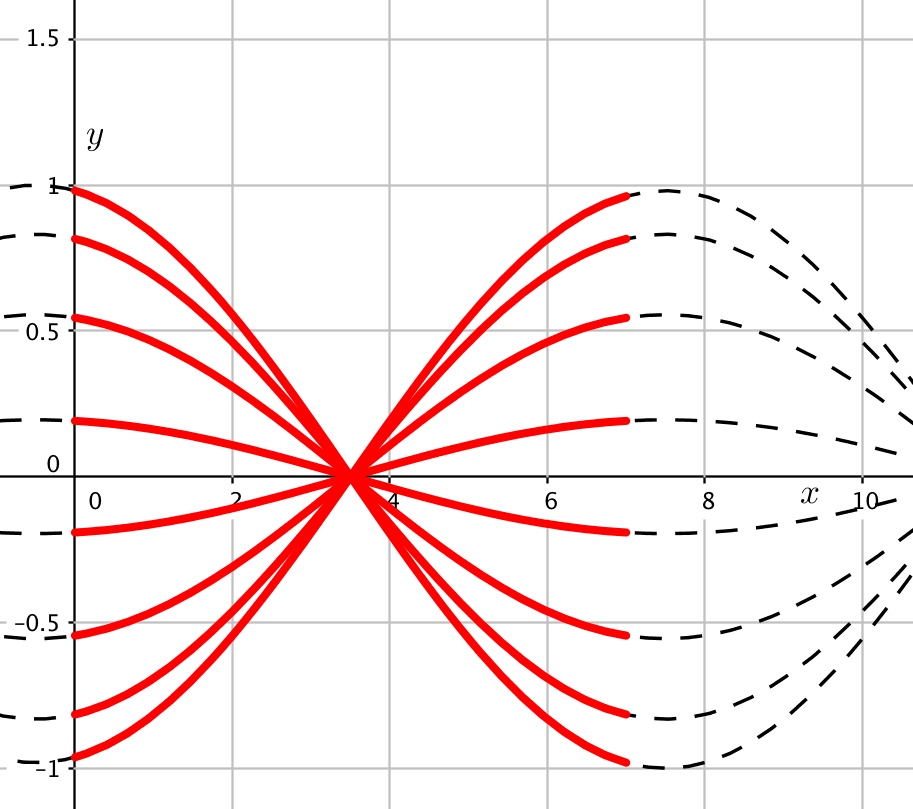
\includegraphics[width=0.6\textwidth]{Billeder/Frekvens-eksempelu1v1.png}
\caption{Bølger for hver række for $T(1,\ 1)$.} %tegnet ved brug af ligning \vref{eq:DCTeq}. På hver af disse bølger ligger 8 ligeligt fordelte koefficienter, som multipliceres med signalværdierne.}
\label{fig:frekeksu1v1}
\end{minipage}
\begin{minipage}[b]{0.5\linewidth}
\centering
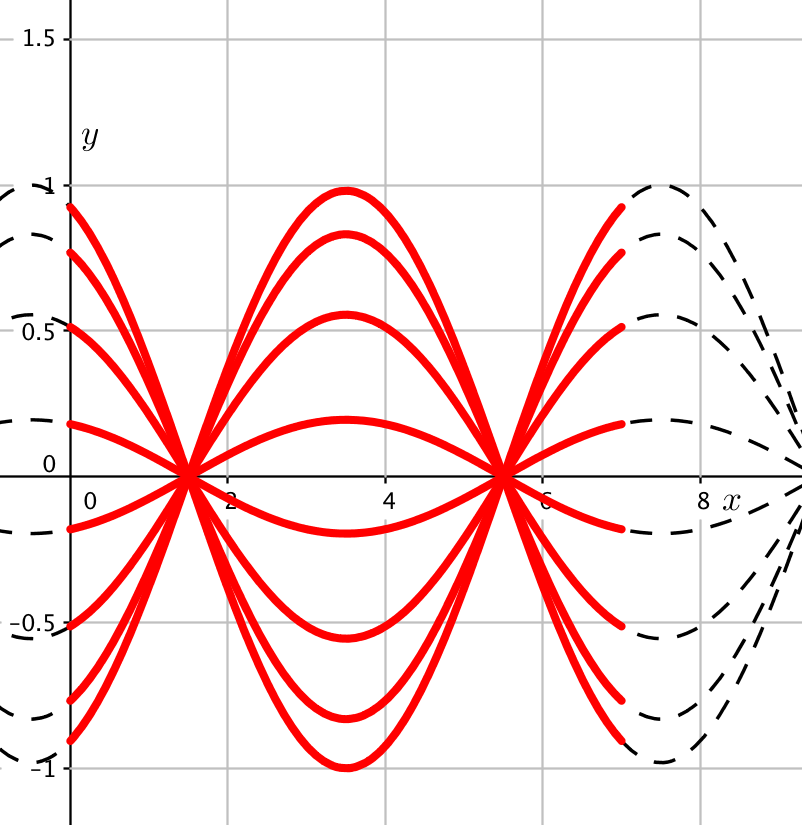
\includegraphics[width=0.5\textwidth]{Billeder/Frekvens-eksempelu1v2.png}
\caption{Bølger for hver række for $T(1,\ 2)$.}
\label{fig:frekeksu1v2}
\end{minipage}
\end{figure}

\begin{figure}[htbp]
\centering
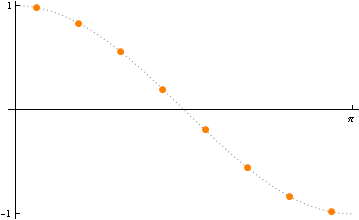
\includegraphics[width=0.4\textwidth]{Billeder/coskoefficienter.png}
\caption{Koefficienterne for $T(1,\ 1)$ og $f(0,\ y)$ afmærket som punkter på en cosinusbølge.}
\label{fig:cosko}
\end{figure}

Det ses desuden på figur \vref{fig:cosko}, at koefficienterne tilsammen har sum lig nul. Der er altså lige mange positive og negative koefficienter i alle bølgerne med undtagelse af den første, som udelukkende består af koefficienten $\frac{\sqrt{2}}{2}$.\\
At hele den første række kun indeholder positive indgange bidrager til energikomprimeringen. Hvis A indeholder lignende værdier, vil indgang $(0,\phantom{i}0)$ have stor numerisk værdi efter transformationen. Derfor kan en stor del af informationerne koncentreres i denne ene indgang. På samme måde vil resultatet af at prikke en vektor med ens indgange, $\vec{v}= \begin{bmatrix} v_1 & v_1 & \hdots & v_1 \end{bmatrix}$ med en hvilken som helst samling af koefficenter fra en cosinusbølge beregnet ved $i=0,\ldots,7$ blive lig nul. Resultatet af at prikke en vektor, med indgange der næsten er ens med koefficienterne, vil blive tæt på eller lig nul [\citet{whydomath_dct}, afsnit 4]

Koefficienten i indgang $(0,\phantom{i}0)$ omtales som DC koefficienten eller Direct Current. De resterende 63 koefficienter kaldes for AC koefficienter eller Alternating Current. Navnene stammer fra transformationens historiske brug i analyse af elektriske kredsløb og refererer til basisfunktionerne i transformationen, som for DC koefficienten er konstant som jævnstrøm, men de oscillerer som vekselstrøm for de resterende koefficienter [\citet{lokminglui_DCT}, s. 5].

De transformerede koefficienter udtrykker bestemte mønstre i signalet. Mønstrene for hver koefficient ses i figur \vref{fig:frekvens_matrix}, hvor bølgetoppene og -dalene i cosinusfunktionerne (og dermed negative og positive koefficienter) er henholdsvis sorte og hvide. Denne figur illustrerer hvordan transformationen behandler forskellige slags mønstre i signalet - mønstre som ligner signalet vil have høje koefficienter. Bemærk at DC koefficienten er en koefficient for et ensfarvet mønster eller signal.
\begin{figure}[htbp]
\centering

\includegraphics[width=0.35\textwidth]{billeder/frekvensmatrix.png}
\caption{Repræsentation af de 64 forskellige basisfunktioner i cosinustransformationen af længde $n = 8$. Mønstrene hører til koefficienterne, som fås ved transformation af et signal. Koefficienternes størrelse fortæller hvor meget, det tilhørende mønster optræder i signalet.}
\label{fig:frekvens_matrix}
\end{figure}
Indgangene i den transformerede matrix er koefficienterne, hvorved disse mønstre er repræsenteret i signalet. Altså kan signalet genskabes ved en lineær kombination af disse mønstre.

I dette projekt udføres beregninger og dermed også transformationen i Python. Til dette er det beregningsmæssigt nemmere og hurtigere at regne med DCT på matrixform.

I udledningen af DCT i appendiks \vref{DCT_udledning} ses formlen for den todimensionelle DCT, hvor ligning \vref{eq:soejlevektor} viser, hvordan hver enkelt søjle i en matrix for en n-punkts DCT beregnes. Da der i denne opgave regnes med matricer af størrelsen $8 \times 8$, vises der i ligning \ref{eq:DCTmatrix} en matrix beregnet ved $n=8$ - altså en $8 \times 8$-matrix.
%\begin{align}
%	y_{(i,j)} = C(i) \sqrt{\frac{2}{n}} \cos\left(\frac{(2 \cdot j-1) \cdot (i-1)\pi}{2n}\right)
%\label{eq:DCTmatrixform}
%\end{align}
%Hvor
%\begin{itemize}
%		\item{$C(i)= \begin{cases}
%			\frac{1}{\sqrt{2}} \ hvis \ i = 1\\
%			1\ \ \ hvis \ i \neq 1
%		\end{cases}
%		$}
%		\item{$y_{(i,j)}=$ indgang $(i,j)$}
%		\item{$n =$ matricens dimensioner n$\times$n}
%\end{itemize}
%Matricen beregnet ved formel \vref{eq:DCTmatrixform} hvor $n=8$ ses i ligning \ref{eq:DCTmatrix}.
\begin{equation}
U=\frac{1}{2}
\begin{bsmallmatrix}
	\frac{\sqrt{2}}{2}	& \frac{\sqrt{2}}{2}		& \frac{\sqrt{2}}{2}		& \frac{\sqrt{2}}{2}		& \frac{\sqrt{2}}{2}		& \frac{\sqrt{2}}{2}		& \frac{\sqrt{2}}{2}		& \frac{\sqrt{2}}{2}		\\
	\cos(\frac{\pi}{16})		& \cos(\frac{3\pi}{16})	& \cos(\frac{5\pi}{16})	& \cos(\frac{7\pi}{16})	& \cos(\frac{9\pi}{16})	& \cos(\frac{11\pi}{16})	& \cos(\frac{13\pi}{16})	& \cos(\frac{15\pi}{16})		\\
	\cos(\frac{2\pi}{16})	& \cos(\frac{6\pi}{16})	& \cos(\frac{10\pi}{16})	& \cos(\frac{14\pi}{16})	& \cos(\frac{18\pi}{16})	& \cos(\frac{22\pi}{16})	& \cos(\frac{26\pi}{16})	& \cos(\frac{30\pi}{16})		\\
	\cos(\frac{3\pi}{16})	& \cos(\frac{9\pi}{16})	& \cos(\frac{15\pi}{16})	& \cos(\frac{21\pi}{16})	& \cos(\frac{27\pi}{16})	& \cos(\frac{33\pi}{16})	& \cos(\frac{39\pi}{16})	& \cos(\frac{45\pi}{16})		\\
	\cos(\frac{4\pi}{16})	& \cos(\frac{12\pi}{16})	& \cos(\frac{20\pi}{16})	& \cos(\frac{28\pi}{16})	& \cos(\frac{36\pi}{16})	& \cos(\frac{44\pi}{16})	& \cos(\frac{52\pi}{16})	& \cos(\frac{60\pi}{16})		\\
	\cos(\frac{5\pi}{16})	& \cos(\frac{15\pi}{16})	& \cos(\frac{25\pi}{16})	& \cos(\frac{35\pi}{16})	& \cos(\frac{45\pi}{16})	& \cos(\frac{55\pi}{16})	& \cos(\frac{65\pi}{16})	& \cos(\frac{75\pi}{16})		\\
	\cos(\frac{6\pi}{16})	& \cos(\frac{18\pi}{16})	& \cos(\frac{30\pi}{16})	& \cos(\frac{42\pi}{16})	& \cos(\frac{54\pi}{16})	& \cos(\frac{66\pi}{16})	& \cos(\frac{78\pi}{16})	& \cos(\frac{90\pi}{16})		\\
	\cos(\frac{7\pi}{16})	& \cos(\frac{21\pi}{16})	& \cos(\frac{35\pi}{16})	& \cos(\frac{49\pi}{16})	& \cos(\frac{63\pi}{16})	& \cos(\frac{77\pi}{16})	& \cos(\frac{91\pi}{16})	& \cos(\frac{105\pi}{16})	\\
\end{bsmallmatrix}
\label{eq:DCTmatrix}
\end{equation}
Magen til ligning \vref{eq:DCTeq} kan $U$ bruges til at opnå DCT transformationen, blot hvor en stor del af udregningerne er udført på forhånd. På matrixform prikkes $U$ med $A$, og derefter prikkes dette resultat med $U^T$. Transformationen ses i ligning \vref{eq:DCTtrans}. %I beregningerne bruges den transponerede matrix, som ses i ligning \Vref{eq:DCTmatrixT}.
%\begin{equation}
%U^T = \frac{1}{2}
%\begin{bmatrix}
%\frac{2}{\sqrt{2}} & \cos(\frac{\pi}{16}) & \cos(\frac{2 \cdot \pi}{16}) & \cos(\frac{3 \cdot \pi}{16}) & \cos(\frac{4 \cdot \pi}{16}) & \cos(\frac{5 \cdot \pi}{16}) & \cos(\frac{6 \cdot \pi}{16}) & \cos(\frac{7 \cdot \pi}{16}) \\
%\frac{2}{\sqrt{2}} & \cos(\frac{3 \cdot \pi}{16}) & \cos(\frac{6 \cdot \pi}{16}) & \cos(\frac{9 \cdot \pi}{16}) & \cos(\frac{12 \cdot \pi}{16}) & \cos(\frac{15 \cdot \pi}{16}) & \cos(\frac{18 \cdot \pi}{16}) & \cos(\frac{21 \cdot \pi}{16}) \\
%\frac{2}{\sqrt{2}} & \cos(\frac{5 \cdot \pi}{16}) & \cos(\frac{10 \cdot \pi}{16}) & \cos(\frac{15 \cdot \pi}{16}) & \cos(\frac{20 \cdot \pi}{16}) & \cos(\frac{25\cdot \pi}{16}) & \cos(\frac{30 \cdot \pi}{16}) & \cos(\frac{35 \cdot \pi}{16}) \\
%\frac{2}{\sqrt{2}} & \cos(\frac{7 \cdot \pi}{16}) & \cos(\frac{14 \cdot \pi}{16}) & \cos(\frac{21 \cdot \pi}{16}) & \cos(\frac{28 \cdot \pi}{16}) & \cos(\frac{35 \cdot \pi}{16}) & \cos(\frac{42 \cdot \pi}{16}) & \cos(\frac{49 \cdot \pi}{16}) \\
%\frac{2}{\sqrt{2}} & \cos(\frac{9 \cdot \pi}{16}) & \cos(\frac{18 \cdot \pi}{16}) & \cos(\frac{27 \cdot \pi}{16}) & \cos(\frac{36 \cdot \pi}{16}) & \cos(\frac{45 \cdot \pi}{16}) & \cos(\frac{54 \cdot \pi}{16}) & \cos(\frac{63 \cdot \pi}{16}) \\
%\frac{2}{\sqrt{2}} & \cos(\frac{11 \cdot \pi}{16}) & \cos(\frac{22 \cdot \pi}{16}) & \cos(\frac{33 \cdot \pi}{16}) & \cos(\frac{44 \cdot \pi}{16}) & \cos(\frac{55 \cdot \pi}{16}) & \cos(\frac{66 \cdot \pi}{16}) & \cos(\frac{77 \cdot \pi}{16}) \\
%\frac{2}{\sqrt{2}} & \cos(\frac{13 \cdot \pi}{16}) & \cos(\frac{26 \cdot \pi}{16}) & \cos(\frac{39 \cdot \pi}{16}) & \cos(\frac{52 \cdot \pi}{16}) & \cos(\frac{65 \cdot \pi}{16}) & \cos(\frac{78 \cdot \pi}{16}) & \cos(\frac{91 \cdot \pi}{16}) \\
%\frac{2}{\sqrt{2}} & \cos(\frac{15 \cdot \pi}{16}) & \cos(\frac{30 \cdot \pi}{16}) & \cos(\frac{45 \cdot \pi}{16}) & \cos(\frac{60 \cdot \pi}{16}) & \cos(\frac{75 \cdot \pi}{16}) & \cos(\frac{90 \cdot \pi}{16}) & \cos(\frac{105 \cdot \pi}{16})
%\end{bmatrix}
%\label{eq:DCTmatrixT}
%\end{equation}
\begin{align}
B=U \cdot A \cdot U^T
\label{eq:DCTtrans}
\end{align}
Hvor
\begin{itemize}
	\item $B$: den transformerede matrix
	\item $U$: DCT-matricen
	\item $A$: $8\times8$ matrix af pixelværdier
\end{itemize}
Denne similærtransformation (similaritet forklares senere på side \pageref{sec:similaritet}) har samme effekt på $8\times8$-matricen som ligning \vref{eq:DCTeq}. Ligning \ref{eq:DCTtrans} kan skrives som en sammensat transformation bestående af to transformationer med henholdsvis $U$ og $U^T$ som standardmatricer. De to transformationer ses i ligning \ref{eq:trans1} og \ref{eq:trans2}.
\begin{align}
T(A)=U \cdot A
\label{eq:trans1}
\end{align}
\begin{align}
Q(A)=A \cdot U^T
\label{eq:trans2}
\end{align}
Den sammensatte transformation ser derfor ud som i ligning \ref{sammensat_transformation}.
\begin{align}
Q(T(A))=U \cdot A \cdot U^T=B
\label{sammensat_transformation}
\end{align}
Fremover refereres der til den transformerede matrix som $B$.
\subsubsection*{Ortonormalitet}\label{sec:ortonormalitet}
$U$ er en ortonormal matrix, hvilket ses i ligning \vref{eq:diff_delta}, hvilket er et specialtilfælde af en ortogonal matrix. For ortogonale matricer gælder, at
\begin{itemize}
	\item{alle ortogonale sæt af vektorer som ikke er nul er lineært uafhængige.}
	\item{vektorerne er ortogonale på hinanden.}
	\item{alle underrum i $\mathbb{R}^n$ indeholder en ortogonal basis.}
	\item{$Z^{-1} = Z^T$ [\citet{linalg}, s. 413].}
\end{itemize}
En ortonormal matrix er en ortogonal matrix, hvor der gælder, at søjlerne er vektorer med længden 1 [\citet{linalg}, s. 374].
\subsubsection*{Bijektivitet og invertibilitet}
Den diskrete cosinustransformation skal være invertibel, da det ellers ikke giver mening at transformere data til et kodomæne, hvorfra det ikke kan lade sig gøre at komme tilbage til domænet. En lineær transformation er kun invertibel, hvis den er bijektiv [\citet{linalg}, s. 555].

En lineær transformation $T:\mathbb{R}^n \longrightarrow \mathbb{R}^n$ med standardmatrix $A$ er invertibel, hvis og kun hvis $A$ er invertibel. I så fald er den inverse transformation $T^{-1}$ og dens standardmatrix er $A^{-1}$ [\citet{linalg}, s. 187].

En lineær transformation $T:\mathbb{R}^n \longrightarrow \mathbb{R}^m$ siges at være bijektiv, hvis den er både surjektiv og injektiv og derved bijektiv [\citet{linalg}, s. 555].

Altså ønskes det at vise, at den diskrete cosinustransformation er bijektiv.

\textbf{Surjektivitet}\\
En lineær transformation $T:\mathbb{R}^n \longrightarrow \mathbb{R}^m$ siges at være surjektiv, hvis transformationens billedmængde er lig kodomænet $\mathbb{R}^n$ [\citet{linalg}, s. 180].

For en surjektiv lineær transformation $T:\mathbb{R}^n \longrightarrow \mathbb{R}^m$ med standardmatrix $A$ gælder, at
\begin{align}
Rank(A)	&	=m\\
Col(A)	&	=\mathbb{R}^m
\end{align} [\citet{linalg}, s. 181]

Da matricen $U$, som er standardmatrix i cosinustransformationen, opfylder de to ovenstående krav på baggrund af, at den er ortonormal og kvadratisk, kan der sluttes, at den lineære transformation med standardmatrix $U$ er surjektiv.

\textbf{Injektivitet}\\
En lineær transformation $T:\mathbb{R}^n \longrightarrow \mathbb{R}^m$ siges at være injektiv, hvis hvert par af særskilte vektorer i domænet $\mathbb{R}^n$ har særskilte billeder i kodomænet $\mathbb{R}^m$ [\citet{linalg}, s. 182].

For en injektiv lineær transformation $T:\mathbb{R}^n \longrightarrow \mathbb{R}^m$ med standardmatrix $A$ gælder, at
\begin{align}
Null(A)	&	=0\\
Rank(A)	&	=n
\end{align} [\citet{linalg}, s. 184]

Da matricen $U$ opfylder de to ovenstående krav på baggrund af, at den er ortonormal og kvadratisk, kan der sluttes, at den lineære transformation med standardmatrix $U$ er injektiv.

Da den lineære transformation med standardmatrix $U$ er både injektiv og surjektiv, er den altså bijektiv. Disse egenskaber gør, at transformationen kan inverteres, som vist i ligning \ref{eq:similaere2}.
\subsubsection*{Similaritet}\label{sec:similaritet}
Som tidligere nævnt er udtryk \ref{eq:DCTtrans} en similærtransformation, og defintionen for similaritet lyder som følgende: To kvadratiske matricer, $A$ og $B$, siges at være similære, hvis der findes en invertibel matrix, $P$, som opfylder
\begin{align}
B=P^{-1} \cdot A \cdot P
\end{align}
Da der gælder at $U^T=U^{-1}$ [\citet{linalg}, s. 413] sluttes, at ligningerne \ref{eq:similaere1} og \ref{eq:similaere2} gælder.
\begin{align}
B = U \cdot A \cdot U^{-1} = U \cdot A \cdot U^T
\label{eq:similaere1}
\end{align}
\begin{align}
A = U^{-1} \cdot B \cdot U = U^T \cdot B \cdot U
\label{eq:similaere2}
\end{align}
Matricerne $A$ og $B$ er altså similære matricer. Transformationen er dermed en similærtransformation \citep{similar_wolfram}. Den diskrete cosinus transformation ses også som værende invertibel ved
\begin{align}
B=U \cdot A \cdot U^T
\end{align}
Da $A$ og $B$ er similære, er transformationen et basisskift da følgende ligning gælder.
\begin{align}
B=P^{-1} \cdot A \cdot P
\end{align}
Hvor
\begin{itemize}
	\item{$A$: $n \times n$-matrix}
	\item{$B$: $n \times n$-matrix}
	\item{$P$: $U^T$}
\end{itemize}
$B$ er altså $A$ udtrykt i basen $U^T$. Basisskiftet gør det nemmere at foretage den tidligere omtalte udvælgelse af vigtige informationer

Hermed er der redegjort for DCT og dens egenskaber, og der bliver i næste sektion vist eksempler på transformation af diverse $8\times8$-matricer, før den videre algoritme forklares.
%Den diskrete cosinus transformation er ydermere invertibel, og den inverse transformation kan let udledes fra transformationen i ligning \vref{eq:DCTtrans} \citep{whydomath_dct}. For at nå frem til den inverse transform benyttes den associative lov om matrixmultiplikation \citep{linalg}.
%\begin{align}
%A \cdot (C \cdot P)=(A \cdot C) \cdot P
%\end{align}
%for matrixdimensioner
%\begin{itemize}
%	\item{$A=k \times m$}
%	\item{$C=m \times n$}
%	\item{$P=n \times p$}
%\end{itemize}
%Med denne regneregel kan den inverse transformation udledes.
%\begin{align}
%A
%\ =I_n \cdot A \cdot I_n
%\ = (U^T \cdot U) \cdot A \cdot (U^T \cdot U)
%\end{align}
%Den associative lov om matrixmultiplikation benyttes.
%\begin{align}
%A=U^T \cdot (U \cdot A \cdot U^T) \cdot U
%\end{align}
%Det ses at udtrykket i parentesen er magen til udtrykket i ligning \vref{eq:DCTtrans}.
%\begin{align}
%A=U^T \cdot B \cdot U
%\label{eq:DCTinvers}
%\end{align}
%Det ses altså at transformationen i ligning \ref{eq:DCTtrans} kan inverteres ved ligning \ref{eq:DCTinvers}.
\subsection{Eksempler på brug af den diskrete cosinustransformation}
For at illustrere hvordan den diskrete cosinustransformation fungerer, vises her eksempler på $8\times8$ matricer transformeret ved den diskrete cosinustransformation. Da billeder er det, der undersøges i dette projekt, vises de respektive $8\times8$ billeder tilhørende matricerne også. Der er trukket 128 fra alle indgange inden transformationen, hvilket bl.a. forsimpler processen med kvantisering - dette uddybes i afsnit \ref{sec:preprocessing}. Alle koefficienter er desuden afrundet til nærmeste heltal efter transformationen, for at gøre matricerne letlæselige. Der gøres opmærksom på, at der kan være koefficienter, som bliver afrundet til nul. Alle koeffiecienter, som er nul, repræsenteres af ".".
\begin{figure}[htbp]
\centering

\includegraphics[width=0.15\textwidth]{Billeder/8x8_eks1.png}
\caption{$8 \times 8$ billede som består udelukkende af pixels med intensitet 100.\label{fig:8x8graa}}
\end{figure}

\begin{figure}[htbp]
\begin{minipage}[b]{0.45\linewidth}
\centering
$\begin{bmatrix}
100	&	100	&	100	&	100	&	100	&	100	&	100	&	100\\
100	&	100	&	100	&	100	&	100	&	100	&	100	&	100\\
100	&	100	&	100	&	100	&	100	&	100	&	100	&	100\\
100	&	100	&	100	&	100	&	100	&	100	&	100	&	100\\
100	&	100	&	100	&	100	&	100	&	100	&	100	&	100\\
100	&	100	&	100	&	100	&	100	&	100	&	100	&	100\\
100	&	100	&	100	&	100	&	100	&	100	&	100	&	100\\
100	&	100	&	100	&	100	&	100	&	100	&	100	&	100
\end{bmatrix}$
\caption{Pixelværdier for figur \ref{fig:8x8graa}.\label{fig:graamatrix}}
\end{minipage}
\hspace{1.0cm}
\begin{minipage}[b]{0.45\linewidth}
\centering
$\begin{bmatrix}
-224		&	.	&	.	&	.	&	.	&	.	&	.	&	.\\
.		&	.	&	.	&	.	&	.	&	.	&	.	&	.\\
.		&	.	&	.	&	.	&	.	&	.	&	.	&	.\\
.		&	.	&	.	&	.	&	.	&	.	&	.	&	.\\
.		&	.	&	.	&	.	&	.	&	.	&	.	&	.\\
.		&	.	&	.	&	.	&	.	&	.	&	.	&	.\\
.		&	.	&	.	&	.	&	.	&	.	&	.	&	.\\
.		&	.	&	.	&	.	&	.	&	.	&	.	&	.\\
\end{bmatrix}
$
\caption{Figur \ref{fig:graamatrix} transformeret.\label{fig:trans_matrix1}}
\end{minipage}
\end{figure}
I figur \ref{fig:graamatrix} har alle indgange en værdi på 100, hvilket svarer til et billede bestående af 64 pixels i samme gråtone med farveintensitet på 100. I figur \ref{fig:8x8graa} ses matricen repræsenteret ved et billede, og i figur \ref{fig:trans_matrix1} ses den transformerede matrix. Det ses at alle koefficienter er lig nul med undtagelse af DC koefficienten, som er lig -224. Altså kan hele det behandlede signal udtrykkes ved indgang $(0, 0)$, da det kun er den første basisfunktion, som bruges til at repræsentere billedet.

I figur \ref{fig:tern_matrix} udtrykkes matricen for et billede, som består af 64 pixels, hvoraf halvdelen er i gråtoner med farveintensitet = 100, og den anden halvdel er hvide med farveintensitet = 255. Det ses i \ref{fig:trans_matrix2}, at koefficienterne er anderledes end i \ref{fig:trans_matrix1} og udtrykker signalet ved andre koefficienter. Denne gang benyttes flere AC koefficienter for at udtrykke signalet, da der er mere variation i signalet.
\begin{figure}[htbp]
\centering

\includegraphics[width=0.15\textwidth]{Billeder/8x8_eks3.png}
\caption{$8 \times 8$ billede bestående af grå og hvide pixels med farveintensiteter på henholdsvis 100 og 255.}
\label{fig:8x8halvgraa}
\end{figure}
\begin{figure}[htbp]
\begin{minipage}[b]{0.45\linewidth}
\centering
$\begin{bmatrix}
100	&	100	&	100	&	100	&	255	&	255	&	255	&	255\\
100	&	100	&	100	&	100	&	255	&	255	&	255	&	255\\
100	&	100	&	100	&	100	&	255	&	255	&	255	&	255\\
100	&	100	&	100	&	100	&	255	&	255	&	255	&	255\\
255	&	255	&	255	&	255	&	100	&	100	&	100	&	100\\
255	&	255 &	255	&	255	&	100	&	100	&	100	&	100\\
255	&	255	&	255	&	255	&	100	&	100	&	100	&	100\\
255	&	255	&	255	&	255	&	100	&	100	&	100	&	100
\end{bmatrix}$
\caption{Pixelværdier for figur \ref{fig:8x8halvgraa}.\label{fig:tern_matrix}}
\end{minipage}
\hspace{1.0cm}
\begin{minipage}[b]{0.45\linewidth}
\centering
$\begin{bmatrix}
396	&	.		&	.	&	.	&	.	&	.	&	.	&	.	\\
.	&	-509		&	.	&	179	&	.	&	119	&	.	&	101	\\
.	&	.		&	.	&	.	&	.	&	.	&	.	&	.	\\
.	&	179		&	.	&	-63	&	.	&	42	&	.	&	-36	\\
.	&	.		&	.	&	.	&	.	&	.	&	.	&	.	\\
.	&	-119		&	.	&	42	&	.	&	-28	&	.	&	24	\\
.	&	.		&	.	&	.	&	.	&	.	&	.	&	.	\\
.	&	101		&	.	&	-36	&	.	&	24	&	.	&	-20
\end{bmatrix}
$
\caption{Figur \ref{fig:tern_matrix} transformeret.\label{fig:trans_matrix2}}
\end{minipage}
\end{figure}
Matricen i figur \ref{fig:trans_matrix2} viser, at når et billede har store og bratte ændringer mellem farveintensiteter, skal der bruges mange cosinusfunktioner til at udtrykke det bratte skift i farveintensitet. Dette er de tilfælde, som cosinusfunktionen ikke behandler godt - der opnås ikke god energikomprimering.

I figur \ref{fig:gradient_matrix} ses en matrix, som laver en glat overgang fra hvid til sort i samme mønster som den i figur \ref{fig:tern_matrix}. Denne glatte overgang skulle gerne være lettere for cosinusfunktionen at energikomprimere, da der ikke sker bratte skift i farveintensitet. Det tilsvarende billede ses i figur \ref{fig:gradient} og den transformerede matrix ses i figur \ref{fig:trans_matrix3}. Af den transformerede matrix ses det, at cosinustransformationen har haft lettere ved at energikomprimere denne matrix end den i figur \ref{fig:tern_matrix}. Det antages, at billeder primært har glatte overgange mellem farveintensiteter, som ligner den i figur \ref{fig:gradient}.
\begin{figure}[htbp]
\centering

\includegraphics[width=0.15\textwidth]{Billeder/8x8_eks6.png}
\caption{$8\times8$ billede bestående af pixels med gradvis overgang fra hvid til sort.}
\label{fig:gradient}
\end{figure}
\begin{figure}[htbp]
\begin{minipage}[b]{0.45\linewidth}
\centering
$\begin{bmatrix}
255	&	236	&	200	&	153	&	102	&	55	&	19	&	0\\
236	&	236	&	200	&	153	&	102	&	55	&	19	&	19\\
200	&	200	&	200	&	153	&	102	&	55	&	55	&	55\\
153	&	153	&	153	&	153	&	102	&	102	&	102	&	102\\
102	&	102	&	102	&	102	&	153	&	153	&	153	&	153\\
55	&	55	&	55	&	102	&	153	&	200	&	200	&	200\\
19	&	19	&	55	&	102	&	153	&	200	&	236	&	236\\
0	&	19	&	55	&	102	&	153	&	200	&	236	&	255
\end{bmatrix}$
\caption{Pixelværdier til figur \ref{fig:gradient}.\label{fig:gradient_matrix}}
\end{minipage}
\hspace{1.0cm}
\begin{minipage}[b]{0.45\linewidth}
\centering
$\begin{bmatrix}
-4	&	.	&	.	&	.	&	.	&	.	&	.	&	.	\\
.	&	568	&	.	&	-40	&	.	&	-4	&	.	&	-1	\\
.	&	.	&	.	&	.	&	.	&	.	&	.	&	.	\\
.	&	-40	&	.	&	54	&	.	&	-11	&	.	&	-1	\\
.	&	.	&	.	&	.	&	.	&	.	&	.	&	.	\\
.	&	-4	&	.	&	-11	&	.	&	24	&	.	&	-5	\\
.	&	.	&	.	&	.	&	.	&	.	&	.	&	.	\\
.	&	-1	&	.	&	-1	&	.	&	-5	&	.	&	22
\end{bmatrix}$
\caption{Figur \ref{fig:gradient_matrix} transformeret.\label{fig:trans_matrix3}}
\end{minipage}
\end{figure}
Den inverse transformation producerer de to originale matricer uden afvigelser. Skridtet er inverterbart og uden tab af informationer.

Opsummeres ovenstående afsnit om DCT er de vigtigste pointer at
\begin{itemize}
\item[...] DCT transformerer fra tidsdomænet til frekvensdomænet
\item[...] DCT på matrixform er udtrykt ved ligningen $B=U \cdot A \cdot U^T$, hvor $U$ er udtrykt ved ligning \vref{eq:DCTtrans}
\item[...] den inverse DCT er udtrykt som $A = U^T \cdot B \cdot U$ 
\end{itemize}

Med DCT-transformationens egenskaber i mente, ses der nu på de resterende elementer i JPEG-komprimeringen. 
\subsection{Forbehandling af billede} \label{sec:preprocessing}
Før billedet transformeres med den diskrete cosinustransformation, skal det forbehandles. Dette indebærer at dele billedet op i undermatricer af $8\times8$ pixels - kvadratiske matricer med 64 indgange. Størrelsen af disse undermatricer af pixels er ikke tilfældig, og har udgangspunkt i egenskaberne ved den diskrete cosinustransformation. Som forklaret i afsnit \vref{sec:teori_intro} antages det, at nærliggende pixels i et billede er korrelerede, og at ikke-nærliggende pixels ikke er korrelerede. Dermed er det formålsløst at forsøge at transformere et helt billede, i håb om at kunne energikomprimere dette. Derfor deles billedet op i mindre undermatricer, og disse transformeres enkeltvis. Den optimale størrelse af disse undermatricer er $8 \times 8$ pixels, hvilket der er flere grunde til.

Matricer af $2\times2$ pixels indeholder ikke nok data for DCT at bearbejde med, og når transformationen skal udtrykke matricen som funktioner af cosinusbølger, er der ikke nok cosinusbølger til at kunne udtrykke matricen til billedet præcist - der er nemlig kun fire. Resultatet er, at datarepræsentationen er upræcist, og at billedet mister for meget kvalitet - det kan ses med det menneskelige øje. Dette skyldes transformationens høje energikomprimering [\citet{guillermo_sapiro}, 19:26-23:52]. Matricer af $4\times4$ lider under tilsvarende problem som $2\times2$ dog i mindre grad.\\
Matricer af $8\times8$ pixels har en størrelse, der gør cosinustransformationen effektiv. Der er nok indgange og dermed cosinusfunktioner til at kunne udtrykke matricen præcist. Desuden kræver energikomprimeringen, at flere pixels kan repræsenteres af enkelte værdier, og det er derfor vigtigt, at de nærliggende pixels ligner hinanden. Hvis dette er tilfældet, hvilket det ofte er i $8 \times 8$ matricer, kan matricen komprimeres. Altså er der nok cosinusfunktioner og nok korrelation mellem de enkelte pixels til, at $8 \times 8$ er en fornuftig størrelse [\citet{guillermo_sapiro}, 19:26-23:52].\\
Årsagerne til ikke at bruge større end $8 \times 8$, som eksempelvis $16\times16$, er flere; det er beregningsmæssigt langt mere effektivt at udføre komprimeringen på mindre matricer - en computer skal bruge færre beregninger, komprimeringsalgoritmen fungerer ud fra princippet om, at nærliggende pixels ligner hinanden, hvilket er mere usandsynligt ved $16 \times 16$ end $8 \times 8$. Cosinustransformationens energikomprimering fungerer bedst, når der er korrelation mellem de pixels, som transformeres - så kan flere pixels udtrykkes ved få værdier i frekvensdomænet. Problemet med at bruge større matricer end $8\times8$ er, at der ikke nødvendigvis er nogen korrelation mellem de enkelte pixels i en stor matrix. Det bliver meget mere sandsynligt, at billedet tydeligt skifter farve over et stort område, og det giver derfor ikke mening at prøve at sammenligne disse pixels, da der sandsyndligvis ikke er nogen korrelation mellem dem [\citet{guillermo_sapiro}, 21:16-21:52].\\
Altså transformeres kun matricer af størrelse $8\times8$ af gangen. Disse kvadratiske matricer af billedet, kaldes som tidligere nævnt $A$. Figur \vref{fig:pixelblok} viser et eksempel på en $8 \times 8$ pixelmatrix. Bemærk at denne matrix kun består af pixels i gråtoner.

Billeder i gråtoner kan deles op som i figur \vref{fig:pixelblok}, og billeder i RGB-farveformatet beskrives med én værdi for hver farve i hver pixel - altså tre værdier. Billeder i farver deles op i de tre farverum, og de enkelte farverum bearbejdes på samme måde som ved gråtoner. Efterfølgende sammensættes de tre farverum igen for at danne billedet.
Hvert farverum opdeles i $A$-matricer, og der subtraheres 128 fra samtlige indgange. Dette gøres for at ændre værdierne fra beliggende i intervallet $[0;255]$ til $[-128;127]$ og dermed centrere dem omkring nul. Dette er ønskværdigt for komprimeringen, da kvantiseringsskridtet dermed efter cosinustransformationen formår at skabe flere ens koefficienter, hvilket gør komprimeringen mere effektiv, men dette uddybes senere.\\
Såfremt billedets dimensioner (både højde og bredde) ikke går op i otte, fyldes de ufuldendte $8 \times 8$ matricer ud med nuller. Dette hedder nulfyldning [\citet{zero_padding}, s. 1]. Nulfyldning er nødvendigt, da DCT i denne rapport bruges på matricer af størrelse $8\times8$, og billedet vil ikke altid have dimensioner, som 8 ikke går op i. Dette resulterer dog i, at der indsættes en grå kant på billedet, som kan give en kontrast til det originale billede, hvilket betyder, at der formentlig opstår større unøjagtigheder i kanten af billedet. Dette har indflydelse på transformationen og dermed hele komprimeringsalgoritmen. Der nøjes dog med at påpege problemet, men ikke lave en bedre løsning end nulfyldning. Det er i det hele taget et grundlæggende problem ved DCT, at transformationen ikke behandler store skift i farveintensitet godt, da den forsøger at udtrykke glatte overgange. Hvis der ikke er glatte overgange, fungerer energikomprimeringen ringe.

Efter forbehandlingen fås en samling af undermatricer bestående af 64 pixels hver, og som tilsammen udgør det komplette billede. Dermed er billedet klar til cosinustransformationen fra forrige sektion.

Ønskes det at invertere forbehandlingsskridtet, skal der indgangsvist adderes med 128 på alle indgange, og det opsplittede billede skal samles fra $8 \times 8$ matricerne til det samlede billede igen. Forbehandlingsskridtet er herved inverteret, hvilket gøres uden tab eller forandringer i dataene.
\subsection{Kvantisering}\label{sec:kvantisering}
Tredje skridt i komprimeringsalgoritmen omhandler kvantisering af de transformerede værdier. Kvantiseringen har til formål at smide de overflødige data væk og desuden gøre billedet klar til fjerde og sidste skridt. Med overflødig data menes der informationer om billedet, som ikke har nogen (eller lille) synlig indflydelse på billedkvaliteten. Da DCT-transformationen har energikomprimeret $A$, repræsenterer de mindste koefficienter de data, der fremkommer mindst i matricen. Da det menneskelige øje har svært ved at se meget hurtige ændringer i farveintensitet over små afstande, er høje frekvensændringer ikke tydelige for det menneskelige øje. Altså er koefficienterne, i nedre højre hjørne af $B$, ikke betydningsfulde for opfattelsen af billedet som helhed.

Kvantiseringen gør brug af indgangsvis division med en $8 \times 8$ matrix (indgang $B_{1,\phantom{i}1}$ divideres med indgang $Q_{1,\phantom{i}1}$ osv.). Denne matrix består af heltal, som  er bestemt empirisk ved eksperimenter omhandlende det menneskelige syn. Tallene i matricen er tilpasset således, at den synlige billedkvalitet er høj, mens billedet komprimeres mest muligt [\citet{lokminglui}, s. 4]. Der findes flere forskellige kvantiseringsmatricer, og den der bruges i dette projekt, er den som bruges i JPEG-standarden [\citet{lokminglui}, s. 4]. Kvantiseringsmatricen, som fremover refereres til som $Q$, ses i ligning \ref{eq:Q50teori}.
\begin{equation}
Q50 =
\begin{bmatrix}
	16	&	11	& 10		& 16		& 	24	&	40	& 51		& 61		\\
	12	&	12	& 14		& 19		& 	26	& 	58	& 60		& 50		\\
	14	&	13	& 16		& 24		& 	40	& 	57	& 69		& 56		\\
	14	&	17	& 22		& 29		& 	51	& 	87	& 80		& 62		\\
	18	&	22	& 37		& 56		& 	68	& 	109	& 103	& 77		\\
	24	&	35	& 55		& 64		& 	81	& 	104	& 113	& 92		\\
	49	&	64	& 78		& 87		& 	103	& 	121	& 120	& 101	\\
	72	&	92	& 95		& 98		& 	112	& 	100	& 103	& 99		\\
\end{bmatrix}
\label{eq:Q50teori}
\end{equation}
Matricen i ligning \vref{eq:Q50teori} hedder $Q50$, fordi den er kvantiseringsmatricen for en komprimering med kvalitet 50 (fremover benævnes Q-værdien blot som eksempelvis $Q50$ eller $Q10$ ved de respektive kvaliteter). I JPEG kan komprimeringsgraden justeres, og det er med denne matrix dette gøres. Matricen kan have en kvalitet mellem 1 og 100, hvor 100 resulterer i laveste komprimering og højeste billedkvalitet, mens 1 omvendt resulterer i højeste komprimering og laveste billedkvalitet. Det er værd at bemærke at $Q50$ ikke komprimerer et billede med 50\% eller 50 gange - værdien er blot et udtryk for en position på en skala fra 1 til 100.\\
For at opnå en anden kvalitet end 50, ændres Q med en bestemt formel. Alt efter den ønskede kvalitet gælder to formler, som begge multiplicerer hver enkelt indgang med en konstant, der beregnes på baggrund af den ønskede kvalitet.
\begin{align}
Q_n=\begin{cases}
	\frac{100-n}{50} \cdot Q50 \ hvis \ n > 50\\
	\frac{50}{n} \cdot Q50 \ \ \ \ \ hvis \ n < 50
\end{cases}
\end{align}
Herunder ses en kvantiseringsmatrix til en kvalitet på 25.
\begin{equation}
Q25 =
\begin{bmatrix}
	32	&	22	& 20		& 32		& 	48	&	80	& 102	& 122	\\
	24	&	24	& 28		& 38		& 	52	& 	116	& 120	& 100	\\
	28	&	26	& 32		& 48		& 	80	& 	114	& 138	& 112	\\
	28	&	34	& 44		& 58		& 	102	& 	174	& 160	& 124	\\
	36	&	44	& 74		& 112	& 	136	& 	218	& 206	& 134	\\
	48	&	70	& 110	& 128	& 	162	& 	208	& 226	& 184	\\
	98	&	128	& 156	& 174	& 	206	& 	242	& 240	& 202	\\
	144	&	184	& 190	& 196	& 	224	& 	200	& 206	& 198	\\
\end{bmatrix}
\label{eq:Q25teori}
\end{equation}
Matricen B kvantiseres ved indgangsvis division med Q.
\begin{align}
C_{(i,\ j)}=\frac{B_{(i,\ j)}}{Q50_{(i,\ j)}}
\label{C_beregning}
\end{align}
Indgangene i $B$ afrundes til nærmeste heltal, og matricen er dermed kvantiseret. Den kvantiserede matrix navngives $C$. Afrundingen gør at komprimeringen mister data, hvilket er et uigenkaldeligt tab af data og kan altså ikke gøres om. Når den komprimerede fil dekomprimeres til et billede, kan det originale billede ikke genskabes, da det inverterede kvantiseringsskridt vil resultere i andre værdier end det originale input, da afrundingen "sletter"\ dataene. Brugen af en ikke-tabsfri komprimering retfærdiggøres ved at de data, som smides væk, ikke har stor betydning for billedets generelle udseende - det menneskelige øje opfatter ikke tydeligt de manglende værdier, når billedet igen dekomprimeres. Desuden gør dette skridt den senere tabsfri komprimering med Huffman væsentligt mere effektiv.

Det ses på $Q$, at indgangene i nederste højre hjørne er væsentligt højere end indgangene i øverste venstre hjørne. Dette resulterer i, at værdier i nederste højre hjørne af $B$ bliver divideret med større tal end i øvre venstre hjørne. Dette betyder imidlertid, at der er større chance for, at tal i nedre højre hjørne bliver afrundet til heltal tæt på eller lig nul, og at værdier i øverste venstre hjørne vil forblive høje i forhold til de øvrige værdier. De mange værdier tæt på eller lig nul skyldes den tidligere centrering omkring nul, da der blev trukket 128 fra alle indgange i $A$. Altså vil $C$ hovedsageligt bestå af nuller og nogle få indgange i øverste venstre hjørne, som ikke er nul.
					
Det ses også, at en højere komprimeringsgrad resulterer i højere heltal i $Q$. Dette gør, at $C$ vil bestå af endnu lavere værdier, og flere vil blive afrundet til nul. Altså vil en endnu større mængde data gå tabt, og billedkvaliteten vil tilsvarende falde. Modsat vil en lavere komprimering resultere i lavere heltal i $Q$ og højere tal i $C$ med færre værdier afrundet til nul. Filen vil i dette tilfælde ende med at fylde mere, men med højere billedkvalitet.

Når dette skridt skal inverteres, ganges $C$ indgangsvis med $Q$-matricen, som blev brugt under komprimeringen.
\begin{align}
B_{(i,\ j)}=C_{(i,\ j)} \cdot Q_{(i,\ j)}
\end{align}
Det er nødvendigt at matricen $Q$, som bruges til inverteringen af skridtet, er magen til den som blev brugt under kvantiseringen. Hvis dette ikke gøres korrekt, vil det lede til værdier i $B$, som ikke ligner de originale, da der ganges med andre tal, end der oprindeligt blev divideret med.

I ligning \ref{fig:kvantiseret} ses et eksempel på en kvantiseret matrix. Matricen som kvantiseres er den fra figur \vref{fig:graamatrix}, og den kvantiseres med $Q50$.
\begin{equation}\resizebox{0.25\textwidth}{!}{$
	C=
\begin{bmatrix}
	2	&	.	& .		& .		& 	.	&	.	& .		& .	\\
	.	&	4	& .		& .		& 	.	& 	.	& .		& .	\\
	.	&	.	& .		& .		& 	.	& 	.	& .		& .	\\
	.	&	1	& .		& .		& 	.	& 	.	& .		& .	\\
	.	&	.	& .		& .		& 	.	& 	.	& .		& .	\\
	.	&	.	& .		& .		& 	.	& 	.	& .		& .	\\
	.	&	.	& .		& .		& 	.	& 	.	& .		& .	\\
	.	&	.	& .		& .		& 	.	& 	.	& .		& .	\\
\end{bmatrix}$}
\label{fig:kvantiseret}
\end{equation}
Her ses det, at mange af koefficienterne er blevet afrundet til nul, og de som ikke er afrundet til nul, er blevet små tal, hvorved matricen er blevet kvantiseret.
\subsection{Entropikodning - Huffmankodning}
\label{sec:Huffman}
Entropikodning som emne vil ikke blive uddybet her, men blot anses som en metode til at definere sandsynligheden af et givent datasæts udkom og repræsentere dette på bedste vis. Der findes flere forskellige entropikodnings-metoder, bl.a. Zigzag- og Huffmankodning. I denne rapport undersøges Huffmankodning. Enkelte grundelementer i grafteori vil dog blive præsenteret, da disse er nødvendige for at forstå Huffmankodning.

Huffmankodning fungerer vha. grafteori, og de nødvendige begreber er [\citet{grafteori}, s. 1-2]:
\begin{itemize}
\item En \emph{knude} er en samling af kanter
\item En \emph{kant} er en forbindelse mellem knuder
\item \emph{Valens} er antallet af kanter, der støder op til en knude
\item Et \emph{blad} er et knude med valens én
\item En \emph{graf} består af knuder og kanter
\item Et \emph{træ} er en sammenhængende graf
\item Et \emph{undertræ} er et afsnit af træet
\item \emph{Sti} er en forbindelse mellem to knuder, hvor alle knuder på stien er forskellige
\end{itemize}
Huffmankodning er en slags entropikodning og er en tabsfri komprimeringsmetode, hvorpå en stor mængde data kan repræsenteres ved hjælp af de enkelte symbolers (i dette tilfælde tallene $0-255$) sandsynlighed for at fremkomme. Komprimering med Huffmankodning tildeler alle symboler, der fremkommer i datastrengen, en bitrepræsentation af variabel længde, der afhænger af symbolets sandsynlighed. Dette betyder at et symbol, der fremkommer mange gange vil være tildelt et kortere kodeord end et symbol, der fremkommer få gange. Herved vil mængden af bits brugt til at repræsentere en datastreng blive nedbragt, da symboler der fremkommer mange gange fylder mindre, end dem der fremkommer få gange. Et kodeord er en binær repræsentation af symbolet og kunne eksempelvis være
\begin{align}
"A: 0, B: 10, C: 110, D: 111"
\label{fx:huffman prefix}
\end{align}
Vigtigt at nævne er, at Huffmankodning er en præfix-fri kode, hvilket betyder, at symboler ikke kan beskrives som sammensætning af andre symboler. Havde eksempel \vref{fx:huffman prefix} været $"A: 0, B: 1, C: 10, D: 11"$, ville en streng af $0$ og $1$ ikke kunne afkodes uden, at kodeordene var synligt adskilt, da det ikke vil være muligt, at se om $10$ betyder B, A eller C. Det er derfor vigtigt i Huffmankodning, at der ikke er nogle præfix for symbolerne, men at koden kan interpreteres entydigt.
\subsubsection{Huffmantræ} \label{sec:huffmanteori}
Huffmankodning foregår vha. skabelsen af et Huffmantræ, som er et overblik over sandsynligheden for, at de enkelte symboler fremkommer, og hvilket kodeord de skal tildeles. Kodeordet er stien ned til bladet. For at forklare skabelsen af et Huffmantræ laves et eksempel bestående af fire symboler, der viser principperne i skabelsen af træet.
Lad os antage at datastrengen lyder $$ abbacdababaccaddabbbacaadabaaddaaccaaaadaadaabaadacaadabaaadacaaadabaa $$ så kan sandsynligheden for at de enkelte symboler fremkomst i datastrengen beregnes. Disse er angivet i tabel \ref{tb:huffman_sandsynlighed}.

Ud fra tabel \vref{tb:huffman_sandsynlighed} opstilles der fire blade med hvert deres symbol som indgang, se figur \vref{fig:huffmantrae_ex1}. Herefter opstilles de to blade med den mindste sandsynlighed i et undertræ med bladene som indgange, se figur \vref{fig:huffmantrae_ex2}. I dette eksempel vil det være bladene for b og c, hvor bladet med mindst sandsynlighed placeres yderst til højre. Hyppigheden af dette undertræ er summen af de to blades sandsynlighed og giver her $0,11+0,16=0,27$. Derudover tildeles kanterne hhv. et nul- og et-tal, som senere bruges til definering af symbolets kodeord. Herefter kigges der på de to blade/undertræer, der har den mindste sandsynlighed, hvilket er undertræet for b,c (samlet sandsynlighed: $0,27$) og d (sandsynlighed: $0,17$). Disse samles i et undertræ, hvor mindste sandsynlighed igen placeres yderst til højre og undertræets samlede sandsynlighed er summen af bladenes sandsynlighed ($0,27+0,17=0,44$), se figur \vref{fig:huffmantrae_ex3}. Samme fremgangsmåde gentages for de sidste to undertræer/blade, og derved skabes det totale og færdige Huffmantræ, se figur \vref{fig:huffmantrae_ex4}.

På baggrund af træet på figur \vref{fig:huffmantrae_ex4} kan symbolernes kodeord defineres som værende stien til de respektive blade, se tabel \vref{tb:huffman_ex}.
\begin{figure}
\centering
\begin{minipage}{0.45\textwidth}
\centering
\begin{tabular}{|c|c|c|} 
\hline
\textbf{Symbol}	&	\textbf{Antal}	&	\textbf{Sandsynlighed}			\\ \hline
a				&	39				&	$\approx  0,56$					\\ \hline
b				&	11				&	$\approx  0,16$					\\ \hline
c				&	8				&	$\approx  0,11$					\\ \hline
d				&	12				&	$\approx  0,17$					\\ \hline
\textbf{Total}	&	\textbf{70}		&	\textbf{$\approx 1$}			\\ \hline
\end{tabular}
\caption{Sandsynligheder for de enkelte symboler\label{tb:huffman_sandsynlighed}}
\end{minipage}
\hspace{0.5cm}
\begin{minipage}{0.45\textwidth}
\centering
\begin{tabular}{|c|c|} 
\hline
\textbf{Symbol}	&	\textbf{Kodeord}	\\ \hline
a		&	0	\\ \hline
b		&	100	\\ \hline
c		&	101	\\ \hline
d		&	11	\\ \hline
\end{tabular}
\caption{Symbolernes kodeord \label{tb:huffman_ex}}
\end{minipage}
\end{figure}
Det er her tydeligt, at symbolerne med størst frekvens er tildelt de korteste binære repræsentationer, hvorved at de pr. symbol vil fylde mindre. Dette er ønskværdigt, når formålet er at bringe filstørrelsen ned.

Hele denne proces kan på samme vis benyttes til at komprimere de kvantiserede værdier i $C$-matricerne fra afsnit \ref{sec:kvantisering}. I disse transformerede og kvantiserede matricer ligger energikomprimerede informationer om det originale billede, således at mange indgange er lig nul. Altså er der mange fremkomster af nul, og disse kan udtrykkes ved en kort binær repræsentation.\\
Når alle værdier er parret med en kodestreng, gemmes disse parringer sammen med en "ordbog"\ (hvilke symboler og kodeord hører sammen) og $Q$. Dermed kan en codec, ved åbning af den komprimerede fil, udpakke og dekomprimere filen til et dekomprimeret billede, som er en efterligning af det originale billede.

Altså er Huffmankodning det mest komprimerende skridt i DCT-algoritmen - de tidligere skridt gør det muligt ved at sørge for, at billedet beskrives med få værdier, og at de resterende værdier er ens. Dette gør Huffmankodningen langt mere effektiv.
\section{DCT anvendelse} \label{sec:DCTAnvendelse}
I dette afsnit undersøges den praktiske anvendelse af DCT, jævnfør kapitel \ref{chapter:DCT}, hvilket udføres på billedet af Lena, se figur \vref{fig:lena-grid-8x8}. Billedet har dimensionerne $ 512 \times \SI{512}{pixel}$, hvilket indledningsvist opdeles i $8 \times 8$ undermatricer. Endvidere er der $ 64 \cdot 64$ matricer af $8 \times 8$, hvilket giver $64 \cdot 64 \cdot 8 \cdot 8 = 512 \cdot 512 = 262.144$ pixels totalt.

De følgende regneoperationer bliver kun udført på den røde farvekanal og første $8 \times 8$ undermatrix for at vise princippet ved brugen af metoden. Ved gentagelse med resten af undermatricerne og de resterende to farvekanaler opnås en komprimering af det fulde farvebillede. Repetitionerne af beregningerne udelades, da dette blot er et eksempel. Derimod \textit{vises} resultatet af komprimeringen for hele billedet, efter regneeksemplet med undermatricen er udført. For at skabe overblik over komprimeringen ses komprimeringsalgoritmen på side \pageref{tb:Algoritme-Komprimering-DCT}
\begin{table}[!h]
\centering
\begin{tabular}{lll}
\hline
\multicolumn{3}{l}{\textbf{Algoritme: Komprimering vha. DCT}}                           \\ \hline
\\
\multicolumn{1}{|l}{1.}        & Input:                     & Billede, $A$: $m \times n$ pixels             \\
\multicolumn{1}{|l}{2.}        & Output:                    & Komprimeret fil       \\
                               &                            &                        \\
\multicolumn{2}{|l}{\textit{Komprimering}}                  &                        \\
\multicolumn{1}{|l}{3.}        & Opdeling:                  & Billede opdeles i farvekanaler og $8 \times 8$ matricer \\
\multicolumn{1}{|l}{4.}        & Centrering omkring 0:      & $A = A - 128$ indgangsvist    \\
\multicolumn{1}{|l}{5.}        & DCT:              & $B = U \boldsymbol{\cdot} A \boldsymbol{\cdot} U^T$  \\
\multicolumn{1}{|l}{6.}        & Kvantisering:              & $C_{(i,\ j)} = \frac{B_{(i,\ j)}}{Q_{(i,\ j)}}$ afrundet\\
\multicolumn{1}{|l}{7.}        & Entropikodning:           & $C$ komprimeres vha. Huffman til en fil              \\
\multicolumn{1}{|l}{8.}        & Gentagelse:                & Ovenstående gentages for samtlige $8 \times 8$ matricer\\
\end{tabular}
\label{tb:Algoritme-Komprimering-DCT}
\end{table}

Den specifikke undermatrix i følgende eksempel ligger i øverste venstre hjørne, jævnfør figur \vref{fig:lena-grid-8x8}. Første værdi for hver indgang, dvs. den røde kanal, findes vha. vores Python-program og følgende undermatrix, $A_{1,1}$, fremkommer.
\begin{figure}[!h]
\begin{minipage}[b]{0.27\linewidth}
\centering

\includegraphics[width=\textwidth]{Billeder/LenaAnvendelse/RED8x8/lena1-R8x8-org.png}
\caption{Oprindelig - Visuel.}
\label{fig:lena1-R8x8-org-visuel}
\end{minipage}
\hspace{0.5cm}
\begin{minipage}[b]{0.45\linewidth}
\centering
\[A_{1,1}=\begin{bmatrix}
226 & 226 & 223 & 223 & 226 & 226 & 228 & 227 \\
226 & 226 & 223 & 223 & 226 & 226 & 228 & 227 \\
226 & 226 & 223 & 223 & 226 & 226 & 228 & 227 \\
226 & 226 & 223 & 223 & 226 & 226 & 228 & 227 \\
226 & 226 & 223 & 223 & 226 & 226 & 228 & 227 \\
227 & 227 & 227 & 222 & 226 & 228 & 226 & 230 \\
228 & 228 & 225 & 224 & 225 & 229 & 229 & 229 \\
223 & 223 & 226 & 221 & 227 & 225 & 226 & 228 \\
\end{bmatrix}\]
\caption{Oprindelig - Tal.}
\label{fig:lena1-R8x8-org-matrix}
\end{minipage}
\end{figure}
\begin{figure}[htbp]
\centering
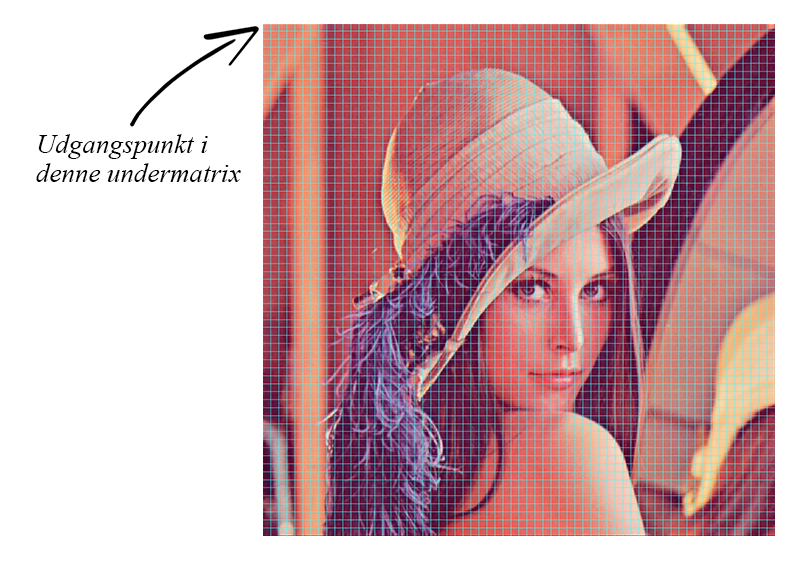
\includegraphics[width=0.5\textwidth]{billeder/lena-grid.png}
\caption{Lena delt op i 4096, $8 \times 8$ undermatricer.}
\label{fig:lena-grid-8x8}
\end{figure}
Herfra udføres DCT på undermatricen, og B findes vha. $B = U \boldsymbol{\cdot} A \boldsymbol{\cdot} U^T$, hvor $U$ og $U^T$ er givet i udtryk \vref{eq:DCTmatrix}.
\begin{figure}[!h]
\begin{minipage}[b]{0.25\linewidth}
\centering

\includegraphics[width=0.9\textwidth]{Billeder/LenaAnvendelse/RED8x8/lena2-R8x8-DCT.png}
\caption{DCT - Visuel.}
\label{fig:lena2-R8x8-DCT-visuel}
\end{minipage}
\hspace{0.5cm}
\begin{minipage}[b]{0.40\linewidth}
\centering
\[B_{1,\ 1}=\begin{bmatrix}
791    & -71  & 8,12   & 4,23   & -1,8  & -3,6  & -1,2  & 2,49   \\
-1,5  & 0,43  & 0,01   & 1,90   & 0,78  & 1,25   & -3,4  & -0,9 \\
-0,7 & -0,8 & -0,7 & -0,9 & -0,1 & -0,2 & 0,93  & 1,02   \\
2,66   & 1,02   & 1,38   & 0,21  & -0,5 & -0,5 & 0,95  & -1,3  \\
-3,3  & -0,9 & -1,5  & -0,2 & 0,75  & 0,18  & -1,0  & 1,55   \\
2,40   & 0,53  & 1,12   & 0,85  & -0,6 & 0,75  & -0,4 & -1,7  \\
-1,1  & -0,1 & -0,6 & -1,3  & 0,32  & -1,4  & 1,75   & 1,50   \\
0,21  & -0,1 & 0,18  & 0,98  & -0,1 & 1,15   & -1,6  & -0,9 \\
\end{bmatrix}\]
\caption{DCT - Tal.}
\label{fig:lena2-R8x8-DCT-matrix}
\end{minipage}
\end{figure}
Det ses tydeligt på den visuelle figur \ref{fig:lena2-R8x8-DCT-visuel}, hvordan alle overflødige høje frekvenser allerede er reduceret kraftigt. Dette er nøjagtigt det, som ønskes af DCT'en, da de lave frekvenser kan ses tydeligere af øjet end de høje. Den visuelle repræsentation er fremkommet ved at trunkere dataene til intervallet $[0;255]$. Næste trin i algoritmen er kvantiseringen, hvor der i dette eksempel tages udgangspunkt i $Q50$ jævnfør \vref{eq:Q50teori}. Den afrundede $C$ findes vha. \vref{C_beregning}
\begin{figure}[!h]
\begin{minipage}[b]{0.25\linewidth}
\centering

\includegraphics[width=0.9\textwidth]{Billeder/LenaAnvendelse/RED8x8/lena3-R8x8-quantization.png}
\caption{Kvantisering - Visuel.}
\label{fig:lena3-R8x8-quantization-visuel}
\end{minipage}
\hspace{0.5cm}
\begin{minipage}[b]{0.40\linewidth}
\centering
\[C_{1,\ 1}=\begin{bmatrix}
49 & -1 & 1 & . & . & . & . & . \\
.  & .  & . & . & . & . & . & . \\
.  & .  & . & . & . & . & . & . \\
.  & .  & . & . & . & . & . & . \\
.  & .  & . & . & . & . & . & . \\
.  & .  & . & . & . & . & . & . \\
.  & .  & . & . & . & . & . & . \\
.  & .  & . & . & . & . & . & . \\
\end{bmatrix}\]
\caption{Kvantisering - Tal.}
\label{fig:lena3-R8x8-quantization-matrix}
\end{minipage}
\end{figure}
Bemærk at der bruges indgangsvis division. Det ses, jævnfør tallene på figur \ref{fig:lena3-R8x8-quantization-matrix}, at matricen hovedsageligt udgøres af nuller. Dette er essentielt for Huffmankodningen, da den nu effektivt kan komprimere. Huffmantræet for undermatricen kan ses på figur \ref{fig:Huffman-8x8-visuel}. Tallene uden parentes repræsenterer hyppigheden af tallene i parentes.
\begin{figure}[htbp]
\centering
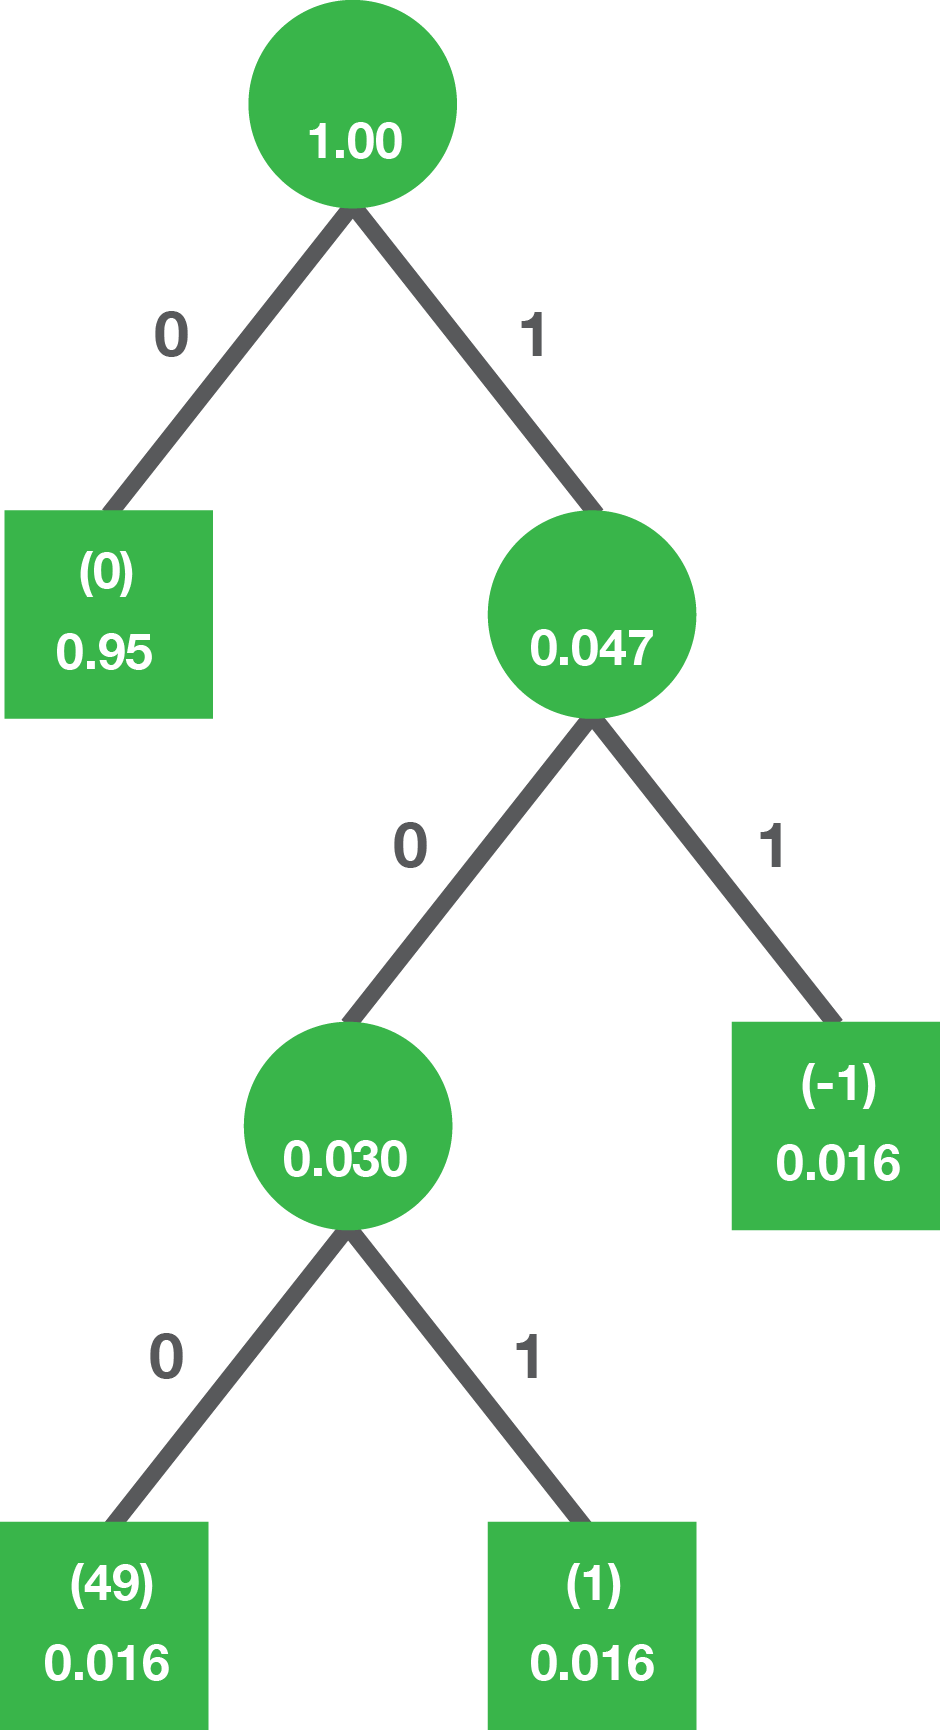
\includegraphics[width=0.25\textwidth]{Billeder/LenaAnvendelse/HUFFMAN/Huffman-8x8.png}
\caption{Huffmantræ for undermatricen.}
\label{fig:Huffman-8x8-visuel}
\end{figure}

Træet havde mildt sagt været markant større, hvis at Huffmantræet var lavet ud fra eksempelvis
 $A_{1,\ 1}$ eller $B_{1,\ 1}$. Her er det åbenlyst hvordan de to nævnte matricer, kun er \textit{forberedende} for en effektiv komprimering.

Der kan med fordel opstilles en tabel med relevante observationer fra Huffmantræet og dens resultater, se tabel \ref{tb:Huffman-8x8}. Den binære form blev fundet jævnfør \vref{sec:huffmanteori}.
\begin{table}[!h]
\centering
\begin{tabular}{|l|l|l|l|}
\hline
\textbf{Indgangsværdi} & \textbf{Antal} & \textbf{Sandsynlighed}      & \textbf{Binær form} \\ \hline
49                & 1              & $\frac{1}{64} \approx 0,016$ & 100                 \\ \hline
1                 & 1              & $\frac{1}{64} \approx 0,016$ & 101                 \\ \hline
-1                & 1              & $\frac{1}{64} \approx 0,016$ & 11                  \\ \hline
0                 & 61             & $\frac{61}{64} \approx 0,95$ & 0                   \\ \hline
\end{tabular}
\caption{Huffmantræet i tabelform}
\label{tb:Huffman-8x8}
\end{table}
I binær form vil undermatricen nu hedde: $$ 100110001010000000000000000000000000000000000000000000000000000000000 $$
En komprimeret fil er opnået, og den lange streng af nuller resulterer i, at filen fylder mindre, end hvis Huffmankodningen var blevet gjort før kvantiseringen. Jævnfør algoritmen på side \pageref{tb:Algoritme-Dekomprimering-DCT} udføres \textit{de}komprimeringen, hvilket gøres med de modsatte regneoperationer i forhold til komprimeringen.
\begin{table}[!h]
\centering
\begin{tabular}{lll}
\hline
\multicolumn{2}{l}{\textbf{Algoritme: Dekomprimering vha. DCT}}    &                                                                   \\ \hline
\\
\multicolumn{1}{|l}{1.}        & Input:                     & Komprimeret fil \\
\multicolumn{1}{|l}{2.}        & Output:                    & Dekomprimeret billede, $A'$                                           \\
                               &                            &                                                                   \\
\multicolumn{2}{|l}{\textit{Dekomprimering (invers proces)}} &                                                                   \\
\multicolumn{1}{|l}{9.}        & Entropidekodning:         & Filen dekomprimeres vha. Huffman til $C'$             \\
\multicolumn{1}{|l}{10.}        & Dekvantisering:            & $B' = Q_{(i,\ j)} \cdot C'_{(i,\ j)}$                                                 \\
\multicolumn{1}{|l}{11.}       & Invers DCT / DCT-III:      & $A' = U^T \boldsymbol{\cdot} B' \boldsymbol{\cdot} U$\\
\multicolumn{1}{|l}{12.}       & Decentrering omkring 0:      & $A' = A' + 128$ indgangsvist\\
\multicolumn{1}{|l}{13.}       & Samling:                   & $8 \times 8$ matricer samles til ét billede
\\  
\end{tabular}
\label{tb:Algoritme-Dekomprimering-DCT}
\end{table}
Resultatet af den inverse algoritme på $A_{(1,\ 1)}$ resulterer i værdierne illustreret i figur \ref{fig:lena4-R8x8-compressed-visuel} og \ref{fig:lena4-R8x8-decompressed-matrix}.
\begin{figure}[htbp]
\begin{minipage}[b]{0.27\linewidth}
\centering

\includegraphics[width=0.8\textwidth]{Billeder/LenaAnvendelse/RED8x8/lena4-R8x8-compressed.png}
\caption{Dekomprimeret - Visuel.}
\label{fig:lena4-R8x8-compressed-visuel}
\end{minipage}
\hspace{0.5cm}
\begin{minipage}[b]{0.45\linewidth}
\centering
\[\resizebox{0.9\textwidth}{!}{$C_{1,\ 1}=\begin{bmatrix}
226 & 225 & 224 & 224 & 225 & 226 & 228 & 230 \\
226 & 225 & 224 & 224 & 225 & 226 & 228 & 230 \\
226 & 225 & 224 & 224 & 225 & 226 & 228 & 230 \\
226 & 225 & 224 & 224 & 225 & 226 & 228 & 230 \\
226 & 225 & 224 & 224 & 225 & 226 & 228 & 230 \\
226 & 225 & 224 & 224 & 225 & 226 & 228 & 230 \\
226 & 225 & 224 & 224 & 225 & 226 & 228 & 230 \\
226 & 225 & 224 & 224 & 225 & 226 & 228 & 230 \\
\end{bmatrix}$}\]
\caption{Dekomprimeret - Tal.}
\label{fig:lena4-R8x8-decompressed-matrix}
\end{minipage}
\end{figure}
Den umiddelbare største ændring af undermatricen er dens endnu mere ensartethed. Da der ikke forekommer drastiske spring i overgangene mellem pixelene ser den monoton ud. Det er svært for det menneskelige øje, at skældne mellem denne undermatrice og den oprindelige, hvilket var intentionen i første omgang. 
For referencens skyld udføres algoritmen på hele Lena i de følgende figurer. Det undlades dog at vise den binære form.
%\begin{figure}[!h]
%\begin{minipage}{0.45\textwidth}
%\centering
%
\includegraphics[width=0.4\textwidth]{Billeder/LenaAnvendelse/LENABILLEDE/lena2-DCT.png}
%\caption{DCT - Lena.}
%\label{fig:lena2-DCT-visuel}
%\end{minipage}
%\hspace{0.5cm}
%\begin{minipage}{0.45\textwidth}
%\centering
%
\includegraphics[width=0.4\textwidth]{Billeder/LenaAnvendelse/LENABILLEDE/lena4-enhanced-quantization2.png}
%\caption{Kvantisering - Lena.}
%\label{fig:lena4-enhanced-quantization-visuel}
%\end{minipage}
%\end{figure}
\begin{figure}[htbp]
\begin{minipage}{0.3\textwidth}
\centering
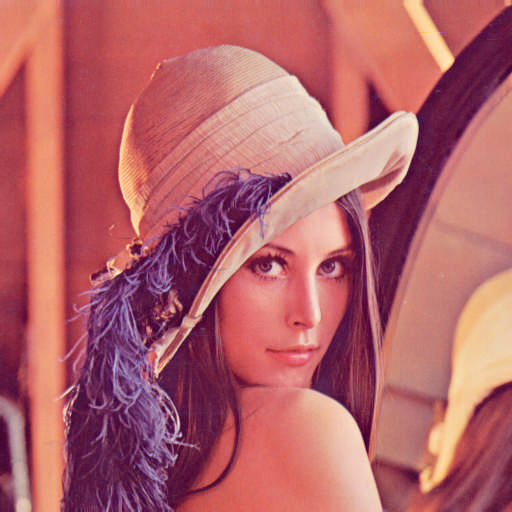
\includegraphics[width=0.9\textwidth]{Billeder/LenaAnvendelse/LENABILLEDE/lena5-compressed.png}
\caption{\href{https://www.dropbox.com/home/P1\%20-\%20B205/vejleder/billeder/DCT/Lena\%20ved\%20forskelige\%20Q?preview=lenaQ50.png}{Dekomprimeret - Lena.}}
\label{fig:lena5-decompressed-visuel}
\end{minipage}
\hspace{0.5cm}
\begin{minipage}{0.3\textwidth}
\centering

\includegraphics[width=0.9\textwidth]{Billeder/fejlbilleder/fejl50.png}
\caption{\href{https://www.dropbox.com/home/P1\%20-\%20B205/vejleder/billeder/DCT/Fejlbilleder?preview=fejl50.png}{Fejlbillede - Lena.}}
\label{fig:lena1-org-fejl}
\end{minipage}
\hspace{0.5cm}
\begin{minipage}{0.3\textwidth}
\centering
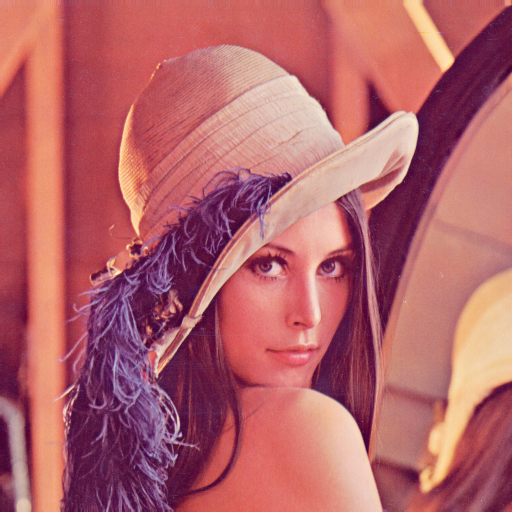
\includegraphics[width=0.9\textwidth]{Billeder/LenaAnvendelse/LENABILLEDE/lena1-org.png}
\caption{\href{https://www.dropbox.com/home/P1\%20-\%20B205/vejleder/billeder?preview=lena-org.tiff}{Oprindelig - Lena.}}
\label{fig:lena1-org-visuel}
\end{minipage}
\end{figure}
Jævnfør \ref{fig:lena5-decompressed-visuel} og \ref{fig:lena1-org-visuel} er det svært at skelne mellem billederne. Dette forstærkes ydermere af fejlbilledet, der illustrerer forskellen mellem det nye og det oprindelige billede. Grå illustrerer ingen forskel, sort illustrerer en mørkere farve i det nye billede, og ligeså illustrerer en lysere farve, at det nye billede er blevet lysere. En farvenuance illustrerer en farveforskel. Hensigten er opnået; billedet har ikke ændret sig betydeligt, og filstørrelsen er komprimeret i forhold til før algoritmen.
%\section{DCT anvendelse} \label{sec:DCTAnvendelse}
I dette afsnit undersøges den praktiske anvendelse af DCT, jævnfør kapitel \ref{chapter:DCT}, hvilket udføres på billedet af Lena, se figur \vref{fig:lena-grid-8x8}. Billedet har dimensionerne $ 512 \times \SI{512}{pixel}$, hvilket indledningsvist opdeles i $8 \times 8$ undermatricer. Endvidere er der $ 64 \cdot 64$ matricer af $8 \times 8$, hvilket giver $64 \cdot 64 \cdot 8 \cdot 8 = 262.144$ pixels totalt.

De følgende regneoperationer bliver kun udført på den røde farvekanal og første $8 \times 8$ undermatrix for at vise princippet ved brugen af metoden. Ved gentagelse med resten af undermatricerne og de resterende to farvekanaler opnås en komprimering af det fulde farvebillede. Repetitionerne af beregningerne udelades, da dette blot er et eksempel. Derimod \textit{vises} resultatet af komprimeringen for hele billedet, efter regneeksemplet med undermatricen er udført. For at skabe overblik over komprimeringen ses komprimeringsalgoritmen herunder:
\begin{table}[!h]
\centering
\begin{tabular}{lll}
\hline
\multicolumn{3}{l}{\textbf{Algoritme: Komprimering vha. DCT}}                           \\ \hline
\\
\multicolumn{1}{|l}{1.}        & Input:                     & Billede, $A$: $m \times n$ pixels             \\
\multicolumn{1}{|l}{2.}        & Output:                    & Komprimeret fil       \\
                               &                            &                        \\
\multicolumn{2}{|l}{\textit{Komprimering}}                  &                        \\
\multicolumn{1}{|l}{3.}        & Opdeling:                  & Billede opdeles i farvekanaler og $8 \times 8$ matricer \\
\multicolumn{1}{|l}{4.}        & Centrering omkring 0:      & $A = A - 128$ indgangsvist    \\
\multicolumn{1}{|l}{5.}        & DCT:              & $B = U \boldsymbol{\cdot} A \boldsymbol{\cdot} U^T$  \\
\multicolumn{1}{|l}{6.}        & Kvantisering:              & $\lfloor C_{(i,\ j)} \rceil = \frac{B_{(i,\ j)}}{Q_{(i,\ j)}}$ afrundet\\
\multicolumn{1}{|l}{7.}        & Entropi kodning:           & $C$ komprimeres vha. Huffman til en fil              \\
\multicolumn{1}{|l}{8.}        & Gentagelse:                & Ovenstående gentages for samtlige $8 \times 8$ matricer\\
\end{tabular}
\label{tb:Algoritme-Komprimering-DCT}
\end{table}

Den specifikke undermatrix i følgende eksempel ligger i øverste venstre hjørne, jævnfør figur \vref{fig:lena-grid-8x8}. Første værdi for hver indgang, dvs. den røde kanal, findes vha. vores Python-program og følgende undermatrix, $A_{1,1}$, fremkommer.

\begin{figure}[!h]
\begin{minipage}[b]{0.27\linewidth}
\centering

\includegraphics[width=\textwidth]{Billeder/LenaAnvendelse/RED8x8/lena1-R8x8-org.png}
\caption{Oprindelig - Visuel.}
\label{fig:lena1-R8x8-org-visuel}
\end{minipage}
\hspace{0.5cm}
\begin{minipage}[b]{0.45\linewidth}
\centering
\[A_{1,1}=\begin{bmatrix}
226 & 226 & 223 & 223 & 226 & 226 & 228 & 227 \\
226 & 226 & 223 & 223 & 226 & 226 & 228 & 227 \\
226 & 226 & 223 & 223 & 226 & 226 & 228 & 227 \\
226 & 226 & 223 & 223 & 226 & 226 & 228 & 227 \\
226 & 226 & 223 & 223 & 226 & 226 & 228 & 227 \\
227 & 227 & 227 & 222 & 226 & 228 & 226 & 230 \\
228 & 228 & 225 & 224 & 225 & 229 & 229 & 229 \\
223 & 223 & 226 & 221 & 227 & 225 & 226 & 228 \\
\end{bmatrix}\]
\caption{Oprindelig - Tal.}
\label{fig:lena1-R8x8-org-matrix}
\end{minipage}
\end{figure}

\begin{figure}[htbp]
\centering
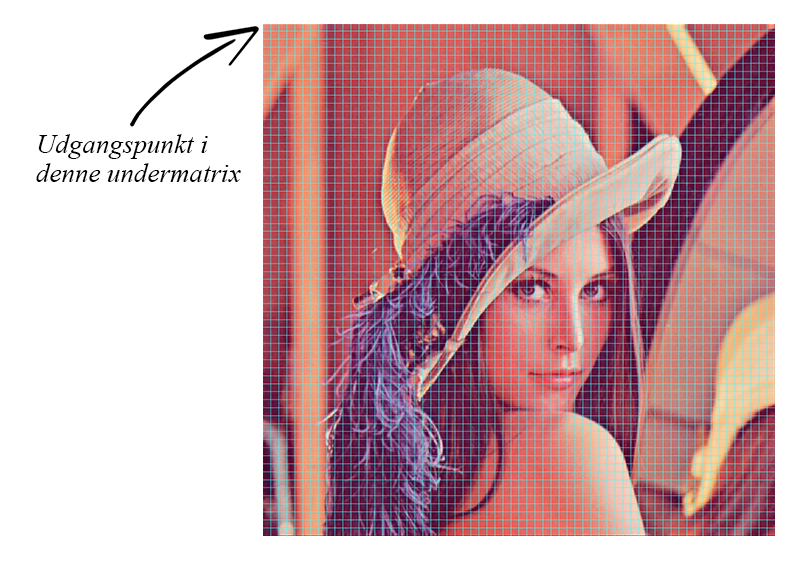
\includegraphics[width=0.7\textwidth]{billeder/lena-grid.png}
\caption{Lena delt op i 4096, $8 \times 8$ undermatricer.}
\label{fig:lena-grid-8x8}
\end{figure}

Herfra udføres DCT på undermatricen, og B findes vha. $B = U \boldsymbol{\cdot} A \boldsymbol{\cdot} U^T$, hvor $U$ og $U^T$ er givet i udtryk \vref{eq:DCTmatrix}.

\begin{figure}[!h]
\begin{minipage}[b]{0.25\linewidth}
\centering

\includegraphics[width=\textwidth]{Billeder/LenaAnvendelse/RED8x8/lena2-R8x8-DCT.png}
\caption{DCT - Visuel.}
\label{fig:lena2-R8x8-DCT-visuel}
\end{minipage}
\hspace{0.5cm}
\begin{minipage}[b]{0.40\linewidth}
\centering
\[B_{1,\ 1}=\begin{bmatrix}
791    & -71  & 8,12   & 4,23   & -1,8  & -3,6  & -1,2  & 2,49   \\
-1,5  & 0,43  & 0,01   & 1,90   & 0,78  & 1,25   & -3,4  & -0,9 \\
-0,7 & -0,8 & -0,7 & -0,9 & -0,1 & -0,2 & 0,93  & 1,02   \\
2,66   & 1,02   & 1,38   & 0,21  & -0,5 & -0,5 & 0,95  & -1,3  \\
-3,3  & -0,9 & -1,5  & -0,2 & 0,75  & 0,18  & -1,0  & 1,55   \\
2,40   & 0,53  & 1,12   & 0,85  & -0,6 & 0,75  & -0,4 & -1,7  \\
-1,1  & -0,1 & -0,6 & -1,3  & 0,32  & -1,4  & 1,75   & 1,50   \\
0,21  & -0,1 & 0,18  & 0,98  & -0,1 & 1,15   & -1,6  & -0,9 \\
\end{bmatrix}\]
\caption{DCT - Tal.}
\label{fig:lena2-R8x8-DCT-matrix}
\end{minipage}
\end{figure}

Det ses tydeligt på den visuelle figur \ref{fig:lena2-R8x8-DCT-visuel}, hvordan alle overflødige høje frekvenser allerede er reduceret kraftigt. Dette er nøjagtigt det, som ønskes af DCT'en, da de lave frekvenser kan ses tydeligere af øjet end de høje. Den visuelle repræsentation er fremkommet ved at trunkere dataene til intervallet $[0;255]$. Næste trin i algoritmen er kvantiseringen, hvor der i dette eksempel tages udgangspunkt i $Q50$ jævnfør \vref{eq:Q50teori}. Den afrundede $C$ findes vha. $\lfloor C_{(i,\ j)} \rceil = \frac{B_{(i,\ j)}}{Q50_{(i,\ j)}}$:

\begin{figure}[!h]
\begin{minipage}[b]{0.25\linewidth}
\centering

\includegraphics[width=\textwidth]{Billeder/LenaAnvendelse/RED8x8/lena3-R8x8-quantization.png}
\caption{Kvantisering - Visuel.}
\label{fig:lena3-R8x8-quantization-visuel}
\end{minipage}
\hspace{0.5cm}
\begin{minipage}[b]{0.40\linewidth}
\centering
\[C_{1,\ 1}=\begin{bmatrix}
49 & -1 & 1 & . & . & . & . & . \\
.  & .  & . & . & . & . & . & . \\
.  & .  & . & . & . & . & . & . \\
.  & .  & . & . & . & . & . & . \\
.  & .  & . & . & . & . & . & . \\
.  & .  & . & . & . & . & . & . \\
.  & .  & . & . & . & . & . & . \\
.  & .  & . & . & . & . & . & . \\
\end{bmatrix}\]
\caption{Kvantisering - Tal.}
\label{fig:lena3-R8x8-quantization-matrix}
\end{minipage}
\end{figure}

Bemærk at der bruges indgangsvis division. Det ses, jævnfør tallene på figur \ref{fig:lena3-R8x8-quantization-matrix}, at matricen hovedsageligt udgøres af nuller. Dette er essentielt for Huffmankodningen, da den nu effektivt kan komprimere. Huffman-træet for undermatricen kan ses på figur \ref{fig:Huffman-8x8-visuel}. Tallene uden parentes repræsenterer hyppigheden af tallene i parentes.
\begin{figure}[htbp]
\centering
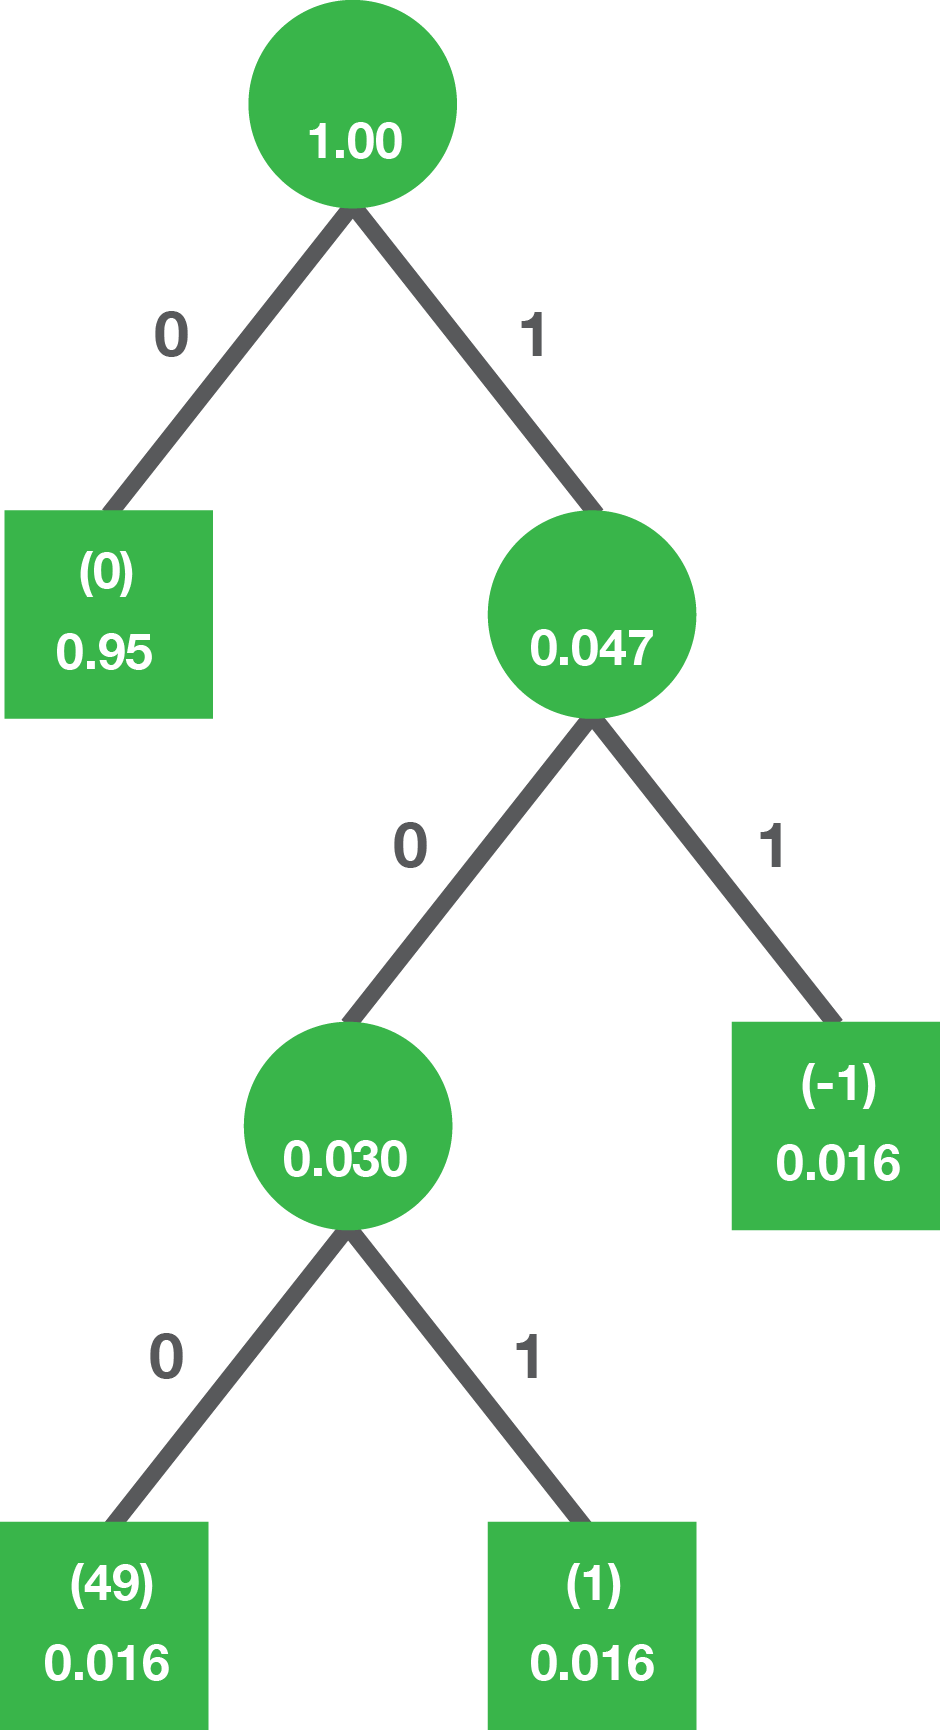
\includegraphics[width=0.25\textwidth]{Billeder/LenaAnvendelse/HUFFMAN/Huffman-8x8.png}
\caption{Huffman-træ for undermatricen.}
\label{fig:Huffman-8x8-visuel}
\end{figure}

Træet havde mildt sagt været markant større, hvis at Huffmantræet var lavet ud fra eksempelvis  $A_{1,\ 1}$ eller $B_{1,\ 1}$. Her er det åbenlyst hvordan de to nævnte matricer, kun er \textit{forberedende} for en effektiv komprimering.

Der kan med fordel opstille en tabel med relevante observationer fra Huffmantræet og dens resultater, se tabel \ref{tb:Huffman-8x8}. Den binære form blev fundet jævnfør \vref{sec:huffmanteori}.

\begin{table}[!h]
\centering
\begin{tabular}{|l|l|l|l|}
\hline
\textbf{Indgangsværdi} & \textbf{Antal} & \textbf{Sandsynlighed}      & \textbf{Binær form} \\ \hline
49                & 1              & $\frac{1}{64} \approx 0,016$ & 100                 \\ \hline
1                 & 1              & $\frac{1}{64} \approx 0,016$ & 101                 \\ \hline
-1                & 1              & $\frac{1}{64} \approx 0,016$ & 11                  \\ \hline
0                 & 61             & $\frac{61}{64} \approx 0,95$ & 0                   \\ \hline
\end{tabular}
\caption{Huffman-træet i tabelform}
\label{tb:Huffman-8x8}
\end{table}

I binær form vil undermatricen nu hedde: $$ 100110001010000000000000000000000000000000000000000000000000000000000 $$
En komprimeret fil er opnået, og den lange streng af nuller resulterer i, at filen fylder mindre, end hvis Huffmankodningen var blevet gjort før kvantiseringen. Jævnfør algoritmen på side \pageref{tb:Algoritme-Dekomprimering-DCT} udføres \textit{de}komprimeringen, hvilket gøres med de modsatte regneoperationer i forhold til komprimeringen.

\begin{table}[!h]
\centering
\begin{tabular}{lll}
\hline
\multicolumn{2}{l}{\textbf{Algoritme: Dekomprimering vha. DCT}}    &                                                                   \\ \hline
\\
\multicolumn{1}{|l}{1.}        & Input:                     & Komprimeret fil \\
\multicolumn{1}{|l}{2.}        & Output:                    & Dekomprimeret billede, $A'$                                           \\
                               &                            &                                                                   \\
\multicolumn{2}{|l}{\textit{Dekomprimering (invers proces)}} &                                                                   \\
\multicolumn{1}{|l}{9.}        & Entropi dekodning:         & Filen dekomprimeres vha. Huffman til $C'$             \\
\multicolumn{1}{|l}{10.}        & Dekvantisering:            & $B' = Q_{(i,\ j)} \cdot C'_{(i,\ j)}$                                                 \\
\multicolumn{1}{|l}{11.}       & Invers DCT / DCT-III:      & $A' = U^T \boldsymbol{\cdot} B' \boldsymbol{\cdot} U$\\
\multicolumn{1}{|l}{12.}       & Decentrering omkring 0:      & $A' = A' + 128$ indgangsvist\\
\multicolumn{1}{|l}{13.}       & Samling:                   & $8 \times 8$ matricer samles til ét billede
\\  
\end{tabular}
\label{tb:Algoritme-Dekomprimering-DCT}
\end{table}

Resultatet af den inverse algoritme på $A_{(1,\ 1)}$ ender med følgende værdierne som illustreret i figur \ref{fig:lena4-R8x8-compressed-visuel} og \ref{fig:lena4-R8x8-decompressed-matrix}.

\begin{figure}[htbp]
\begin{minipage}[b]{0.27\linewidth}
\centering

\includegraphics[width=\textwidth]{Billeder/LenaAnvendelse/RED8x8/lena4-R8x8-compressed.png}
\caption{Dekomprimeret - Visuel.}
\label{fig:lena4-R8x8-compressed-visuel}
\end{minipage}
\hspace{0.5cm}
\begin{minipage}[b]{0.45\linewidth}
\centering
\[C_{1,\ 1}=\begin{bmatrix}
226 & 225 & 224 & 224 & 225 & 226 & 228 & 230 \\
226 & 225 & 224 & 224 & 225 & 226 & 228 & 230 \\
226 & 225 & 224 & 224 & 225 & 226 & 228 & 230 \\
226 & 225 & 224 & 224 & 225 & 226 & 228 & 230 \\
226 & 225 & 224 & 224 & 225 & 226 & 228 & 230 \\
226 & 225 & 224 & 224 & 225 & 226 & 228 & 230 \\
226 & 225 & 224 & 224 & 225 & 226 & 228 & 230 \\
226 & 225 & 224 & 224 & 225 & 226 & 228 & 230 \\
\end{bmatrix}\]
\caption{Dekomprimeret - Tal.}
\label{fig:lena4-R8x8-decompressed-matrix}
\end{minipage}
\end{figure}

Den umiddelbare største ændring af undermatricen er dens endnu mere ensartethed. Da der ikke forekommer drastiske spring i overgangene mellem pixelene ser den monoton ud. Det er svært for det menneskelige øje, at skældne mellem denne undermatrice og den oprindelige, hvilket var intentionen i første omgang. 
For referencens skyld udføres algoritmen på hele Lena-billedet i de følgende figurer. Det undlades dog at vise den binære form.

%\begin{figure}[!h]
%\begin{minipage}{0.45\textwidth}
%\centering
%
\includegraphics[width=0.4\textwidth]{Billeder/LenaAnvendelse/LENABILLEDE/lena2-DCT.png}
%\caption{DCT - Lena.}
%\label{fig:lena2-DCT-visuel}
%\end{minipage}
%\hspace{0.5cm}
%\begin{minipage}{0.45\textwidth}
%\centering
%
\includegraphics[width=0.4\textwidth]{Billeder/LenaAnvendelse/LENABILLEDE/lena4-enhanced-quantization2.png}
%\caption{Kvantisering - Lena.}
%\label{fig:lena4-enhanced-quantization-visuel}
%\end{minipage}
%\end{figure}
\begin{figure}[htbp]
\begin{minipage}{0.3\textwidth}
\centering
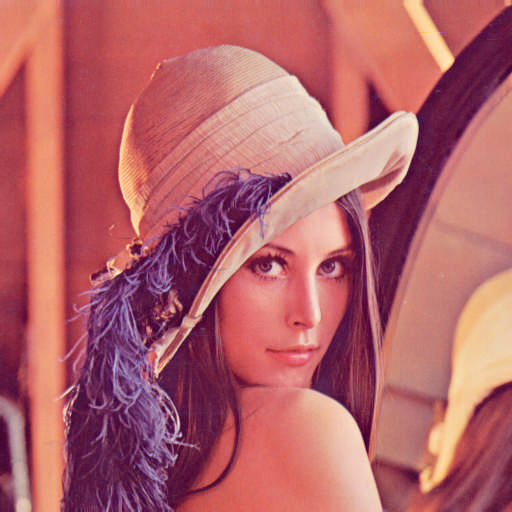
\includegraphics[width=0.9\textwidth]{Billeder/LenaAnvendelse/LENABILLEDE/lena5-compressed.png}
\caption{\href{https://www.dropbox.com/home/P1\%20-\%20B205/vejleder/billeder/DCT/Lena\%20ved\%20forskelige\%20Q?preview=lenaQ50.png}{Dekomprimeret - Lena.}}
\label{fig:lena5-decompressed-visuel}
\end{minipage}
\hspace{0.5cm}
\begin{minipage}{0.3\textwidth}
\centering

\includegraphics[width=0.9\textwidth]{Billeder/fejlbilleder/fejl50.png}
\caption{\href{https://www.dropbox.com/home/P1\%20-\%20B205/vejleder/billeder/DCT/Fejlbilleder?preview=fejl50.png}{Fejlbillede - Lena.}}
\label{fig:lena1-org-fejl}
\end{minipage}
\hspace{0.5cm}
\begin{minipage}{0.3\textwidth}
\centering
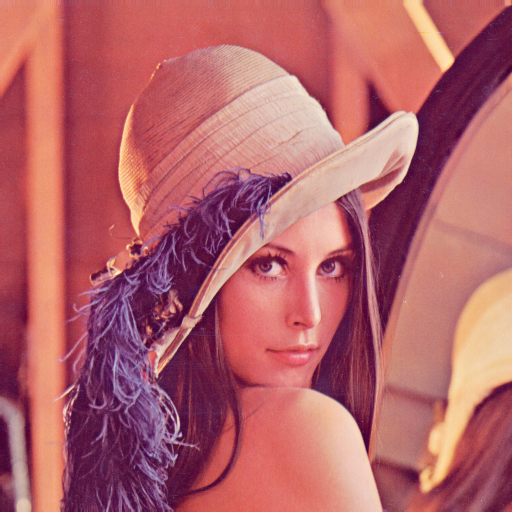
\includegraphics[width=0.9\textwidth]{Billeder/LenaAnvendelse/LENABILLEDE/lena1-org.png}
\caption{\href{https://www.dropbox.com/home/P1\%20-\%20B205/vejleder/billeder?preview=lena-org.tiff}{Oprindelig - Lena.}}
\label{fig:lena1-org-visuel}
\end{minipage}
\end{figure}

Jævnfør \ref{fig:lena5-decompressed-visuel} og \ref{fig:lena1-org-visuel} er det enormt svært at skelne mellem billederne. Dette forstærkes ydermere af fejlbilledet, der illustrerer forskellen mellem det nye og det oprindelige billede. Grå illustrerer ingen forskel, sort illustrerer en mørkere farve i det nye billede, og ligeså illustrerer en lysere farve, at det nye billede er blevet lysere. En farvenuance illustrerer en farveforskel. Hensigten er opnået; billedet har ikke ændret sig betydeligt, og filstørrelsen er komprimeret i forhold til før algoritmen.


%% PCA %%

\chapter{Billedkomprimering med diskret cosinustransformation} \label{chapter:DCT}
I dette kapitel udarbejde en billedkomprimeringsalgoritme med tab med udgangspunkt i den
en diskret cosinustransformation. Før denne forklares, er det nødvendigt at undersøge
den diskrete Fouriertransformation, som den stammer fra.
\section{Diskret Fouriertransformation}
Inden for signalbehandling er den Diskrete Fouriertransformation (DFT) et kendt værktøj. Transformationen er en lineær transformation, som udtrykker et signal på bølgeform ved sinus- og cosinusfunktioner [\citet{thefouriertransform}, afsnit 1]. De fleste signaler er på bølgeform og kan derfor beskrives ved sinus- og cosinusfunktioner gennem DFT.\\
Signalerne kan beskrives i to domæner
\begin{itemize}
\item \textit{Tidsdomænet}\\
		Signalet beskrives ved funktionsværdier til tiden $t$, $f(t)$.
\item \textit{Frekvensdomænet}\\
		Signalet beskrives ved amplitude og fase for en frekvensfunktion.
\end{itemize}
Regneoperationer i tidsdomænet har tilsvarende regneoperationer i frekvensdomænet, som ofte er beregningsmæssigt simplere [\citet{nbtwiki}, afsnit 2]. Af denne grund bruges den diskrete Fouriertransformation til signalbehandling.\\
Transformationen har desuden den egenskab, at den energikomprimerer signalet, som behandles. Energikomprimering betegner en transformations evne til at udtrykke mange signalværdier med høje korrelationer i domænet som færre koefficienter med lav korrelation i kodomænet [\citet{smcnus_energy}, s. 1]. Koefficienterne i frekvensdomænet fortæller i hvor høj grad de enkelte basisfunktioner er repræsenteret i tidsdomænet - høje koefficienter viser en høj optræden af den tilhørende basisfunktion, mens lave koefficienter viser en lav optræden af den tilhørende basisfunktion.

Når DFT udtrykker korrelerede signalværdier som ukorrelerede koefficienter i frekvensdomænet, betyder det også, at transformationen ikke formår at lave energikomprimering i høj grad, hvis signalværdierne er ukorrelerede. Dette betyder at, hvis der ønskes høj energikomprimering, skal DFT kun bruges på signaler, som består af korrelerede værdier.

I billedkomprimering er det, som tidligere beskrevet, interessant at udtrykke et billede ved færre værdier, da der derfor er færre værdier at gemme. DFT kan være et værktøj til dette. Et billede  består netop af korrelerede værdier og DFT kan derfor bruges.

Det viser sig imidlertid, at der findes et bedre værktøj til transformation af korrelerede signalværdier til ukorrelerede koefficienter. Transformationen kaldes den diskrete cosinustransformation (DCT), og er udledt fra DFT [\citet{dft_argument}, s. 3]. Udledningen ses i appendiks \vref{DCT_udledning}.\\
DCT udmærker sig inden for billedbehandling på flere områder i forhold til DFT:
\begin{enumerate}
\item \textit{Energikomprimering}\\
	DCT opnår højere energikomprimering end DFT [\citet{smcnus_energy}, s. 3 og 5]. Den formår at udtrykke informationer om signalværdier i tidsdomænet som færre koefficienter i frekvensdomænet end DFT formår. Det er ønskværdigt at udtrykke mange informationer ved få koefficienter i billedkomprimering.
\item \textit{Reelle tal}\\
	DCT benytter sig udelukkende af reelle tal i de transformerede koefficienter, hvorimod DFT benytter sig af både reelle og komplekse tal som koefficienter. Det er ønskværdigt, at regne udelukkende med reelle tal, da dette forsimpler den videre behandling af signalet.
\end{enumerate}
Der findes desuden en transformation, som bygger på sinusfunktioner - den diskrete sinustransformation (DST). Denne transformerer også signalværdier om til frekvenskoefficienter, men energikomprimerer ikke godt - den er ringere end både DFT og DCT [\citet{smcnus_energy}, s. 5].

Som følge af ovenstående grunde er der valgt at bruge DCT i den mest udbredte open-source komprimeringsstandard; JPEG.\\
På baggrund af at DCT
\begin{itemize}
\item[-] har bedre energikomprimering end DFT [\citet{smcnus_energy}, s. 5], og dermed skal færre koefficienter end DFT bruges til at danne en god approksimation af et signal [\citet{dft_argument}, s. 5]
\item[-] ofte bruges i billedbehandling [\citet{DTT}, s. 1]
\item[-] bruges i JPEG [\citet{dft_argument}, s. 1]
\end{itemize}
tages der i denne opgave udgangspunkt i DCT til at udføre billedkomprimeringer.
\subsection{JPEG}
Joint Photographic Experts Group udgav i 1992 den første JPEG-standard, som komprimerede og dekomprimerede billeder efter en bestemt algoritme. Et program, som kan gøre dette, kaldes en codec. Standarden er open source, og er siden 1992 blevet forbedret flere gange. I denne rapport undersøges en simpel og tidlig version.\\
JPEG gør brug af fire skridt i sin algoritme for at komprimere et billede fra dets fulde størrelse til en fil af mindre størrelse. Den inverse algoritme bruges til at dekomprimere en JPEG-fil til et billede. Da JPEG er en ikke-tabsfri komprimeringsalgoritme, er det dekomprimerede billede kun en efterligning af det originale. [\citet{whydomath_basic}, afsnit 1-7].\\
De fire skridt, som forklares nærmere i et senere afsnit, ser ud som følgende
\begin{enumerate}
\item \textit{Forbehandling af billede}\\
	Forbehandlingen indebærer at dele billedet op i kvadratiske undermatricer af 64 pixels. Dette gøres for at gøre den videre behandling af billedet med den diskrete cosinustransformation mere effektiv. Derudover trækkes 128 fra hver indgang i hver undermatrix for at centrere undermatricerne omkring nul.
\item \textit{Diskret cosinustransformation}\\
	Den diskrete cosinustransformation energikomprimerer billedet ved at udtrykke korrelerede signalværdier som dekorrelerede koefficienter i frekvensdomænet.
\item \textit{Kvantisering}\\
	Kvantiseringen fjerner mindre vigtige informationer om billedet ved at fjerne de dekorrelerede koefficienter, som ikke er vigtige i forhold til de korrelerede signalværdier. Dette skridt gør algoritmen ikke-tabsfri.
\item \textit{Entropikodning}\\
	Entropikodningen opstiller en statistisk model over de kvantiserede koefficienter og koder dem i strenge bestående af 0 og 1, som kan gemmes effektivt i en fil, som er mindre end den oprindelige billedfil.
\end{enumerate}
For at forstå hvorfor og hvordan algoritmen virker er det nødvendigt først at forstå den diskrete cosinustransformation. Derfor bliver dette skridt forklaret først.
\subsection{Diskret Cosinustransformation}\label{sec:DCT}
En diskret cosinustransformation er en lineær transformation, som afbilder en $n$-dimensionel vektor fra domænet $\mathbb{R}^n$ til kodomænet $\mathbb{R}^n$ - altså har transformationen samme kodomæne som domæne. Basisvektorerne i transformationen udledes fra cosinusfunktioner med forskellige frekvenser. Som følge af dette bliver den $n$-dimensionelle vektor afbildet ind i frekvensdomænet - den udtrykkes som en sum af cosinusfunktioner med forskellige frekvenser. Et eksempel på en funktion udtrykt ved bølgefunktioner ses i figur \vref{fig:frequencydomain}.

Som tidligere nævnt er den diskrete cosinustransformation udledt fra den diskrete Fouriertransformation. Udledningen ses i appendiks \vref{DCT_udledning}.

DCT bruges i udstrakt grad i signalbehandling på grund af dens høje energikomprimering. DCT kan altså komprimere meget signalværdi ned til få værdier i frekvensdomænet og dermed udtrykke signalværdier med stor korrelation som koeffiencienter med lav eller ingen korrelation [\citet{lokminglui_DCT}, s. 1]. Transformationen fungerer dog bedst, når signalværdierne som transformeres, har en vis korrelation - hvis dette ikke er tilfældet, vil der ikke blive opnået gode resultater med transformationen.

DCT er imidlertid ikke den eneste transformation, som kan dekorrelere signalværdier. En anden kendt transformation er Karhunen-Loève transformationen. Denne transformation transformerer som cosinustransformationen også korrelerede koefficienter til dekorrelerede koefficienter. Karhunen-Loeve udmærker sig ved at tilpasse sig hvordan signalet ser ud, for således at kunne energikomprimere meget effektivt - transformationen afhænger altså af signalet. Dette gør transformationen i stand til at lave den mest effektive energikomprimering [\citet{lokminglui_DCT}, s. 15]. Det er imidlertid ikke tidsmæssigt effektivt at komponere en ny transformation, hver gang et nyt signal behandles og derfor bruges den diskrete cosinustransformation i JPEG. Denne har en algoritme, som genererer en generel transformation, der kan bruges på mange datasæt [\citet{electronic_engineering}, s. 2].

Da DCT er en lineær transformation, kan den bruges i billedbehandling til at energikomprimere digitale billeder, som har stor korrelation mellem nærliggende pixels.\\
\begin{figure}[htbp]
\centering
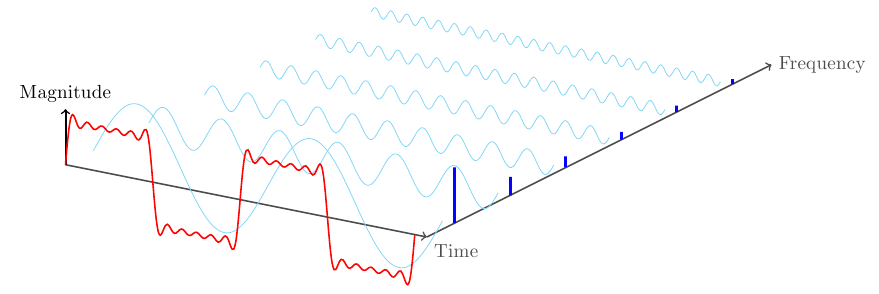
\includegraphics[width=0.7\textwidth]{Billeder/frequencydomain.png}
\caption{Signal (rød) og cosinusbølger (blå kurver) samt amplituden (søjler)[\citet{frequency_image}, \textit{Update 1}].}
\label{fig:frequencydomain}
\end{figure}
Den diskrete cosinustransformation, som kan udledes fra den diskrete Fouriertransformation, kan transformere i både én og to dimensioner. I denne opgave benyttes den todimensionelle. I ligning \vref{eq:DCTeq} ses den todimensionelle $n$-punkt diskrete cosinustransformation, hvor $T:\mathbb{R}^n \longrightarrow \mathbb{R}^n$ transformerer til en matrix indeholdende dekorrelerede koeffecienter. Matricen der transformeres, vil fremover refereres til som $A$. 
\begin{equation}
T_{(i,\ j)}=\sum\limits_{x=0}^{n-1} \sum\limits_{y=0}^{n-1} f(x,\ y) \cdot \alpha(i) \cdot \alpha(j) \cdot \cos\left(\frac{(2x+1) \cdot i \cdot \pi}{2n}\right) \cdot \cos\left(\frac{(2y+1) \cdot j \cdot \pi}{2n}\right)
\label{eq:DCTeq}
\end{equation} [\citet{guillermo_sapiro}, 7:12-11:10]\\
Hvor
\begin{itemize}
\item $T_{(i,\ j)}:$ indgang $(i,\ j)$ i den transformerede matrix ved DCT
\item $f(x,\ y):$ indgang $(x,\ y)$ i A
\item $n:$ matricens dimension
\item $\alpha(i)=\alpha(j)= \begin{cases}
					\sqrt{\frac{1}{n}} \ hvis \ i = 0\\
					\sqrt{\frac{2}{n}} \ hvis \ i \neq 0
					\end{cases}$
\end{itemize}
Det er værd at bemærke, at indgangene i matricen går fra $(0,\ 0)$ til $(n-1,\ n-1)$ i en $n \times n$ matrix. Ydermere er $\alpha(i)$  og $\alpha(j)$ normaliseringsfaktorer [\citet{normalization}, s. 96].

Ligning \ref{eq:DCTeq} bruges i denne opgave ikke til at beregne de transformerede koefficienter, da det beregningsmæssigt ikke er effektivt. Til dette bruges i stedet cosinustransformationen på matrixform, hvilket uddybes senere i dette afsnit. Ligning \ref{eq:DCTeq} er imidlertid god til at illustrere princippet bag transformationen, da det er tydeligt, hvordan cosinusfunktioner indgår i transformationen. Dette undersøges nu.

Det ses af ligning \vref{eq:DCTeq}, at hver transformeret indgang er summen af produktet af de 64 indgange i $A$ og en koefficient fra en cosinusfunktion. For hver række $f(x,\ y)$ holdes $x$ konstant gennem de otte søjler, hvor $y$ går fra $0-7$. Dette giver koefficienter, der alle ligger på en cosinuskurve. Hver gang en ny række $x$ påbegyndes, ændres amplituden af cosinusbølgen, som koefficienterne ligger på. Når en ny transformeret indgang $T_{(i,\ j)}$ beregnes, ændres $i$ og/eller $j$, og frekvensen af cosinusfunktionerne i transformen bliver højere. Altså bliver hver transformeret indgang et unikt aftryk af forskelligt svingene cosinusfunktioner og værdierne i matricen til billedet $A$.

For at illustrere princippet bag de skiftende amplituder og frekvenser af cosinusbølgerne som koefficienterne ligger på, er et sæt af to grafer for cosinustransformationen illustreret i figurerne \ref{fig:frekeksu1v1} og \ref{fig:frekeksu1v2}. Disse er tegnet ved brug af transformationen i ligning \vref{eq:DCTeq} for henholdsvis $T(1,\ 1)$ og $T(1,\ 2)$ og for $n=8$. For hver af funktionerne fremkommer otte bølger, og på hver af disse ligger de otte koefficienter ligeligt fordelt. På figur \ref{fig:cosko} ses de otte punkter på én af bølgerne for $T(0,\ 0)$ [\citet{whydomath_dct}, afsnit 3].

\begin{figure}[!h]
\begin{minipage}[b]{0.5\linewidth}
\centering
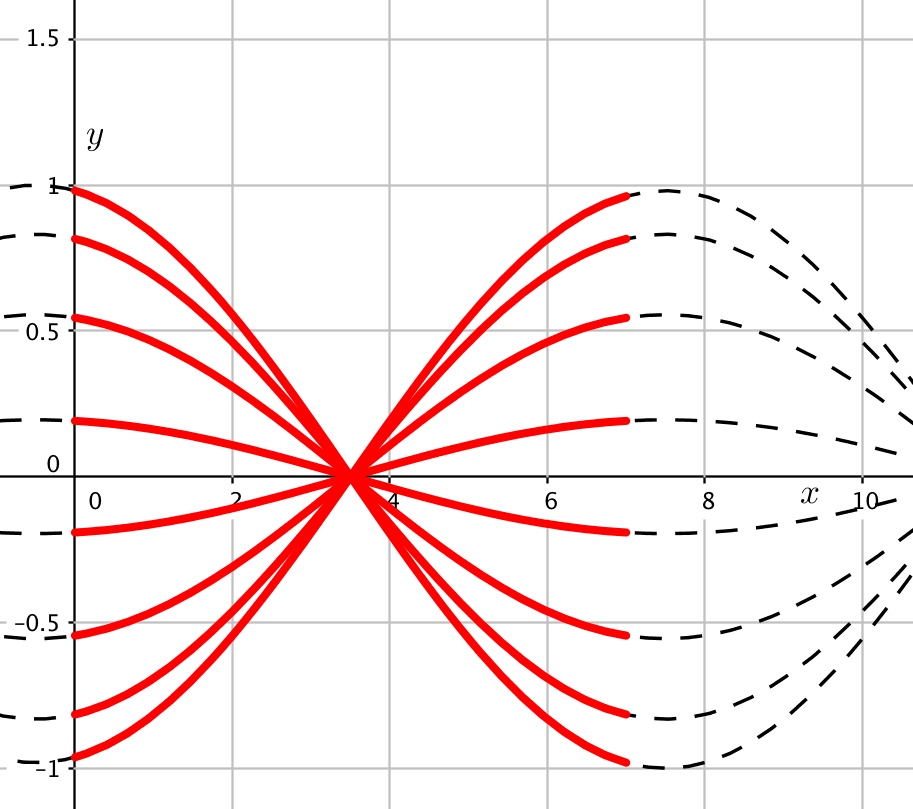
\includegraphics[width=0.6\textwidth]{Billeder/Frekvens-eksempelu1v1.png}
\caption{Bølger for hver række for $T(1,\ 1)$.} %tegnet ved brug af ligning \vref{eq:DCTeq}. På hver af disse bølger ligger 8 ligeligt fordelte koefficienter, som multipliceres med signalværdierne.}
\label{fig:frekeksu1v1}
\end{minipage}
\begin{minipage}[b]{0.5\linewidth}
\centering
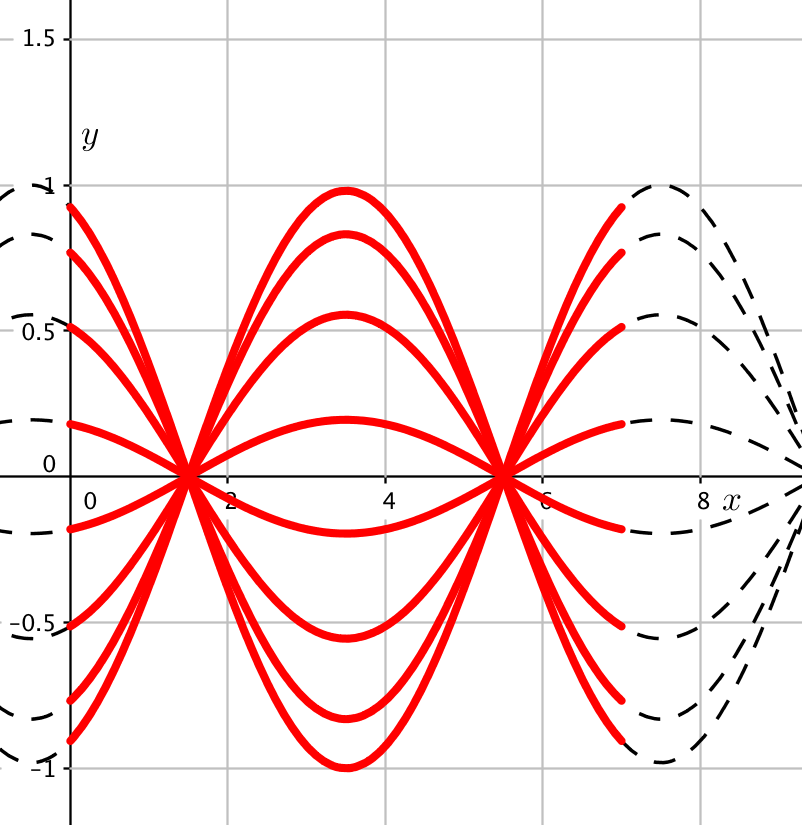
\includegraphics[width=0.5\textwidth]{Billeder/Frekvens-eksempelu1v2.png}
\caption{Bølger for hver række for $T(1,\ 2)$.}
\label{fig:frekeksu1v2}
\end{minipage}
\end{figure}

\begin{figure}[htbp]
\centering
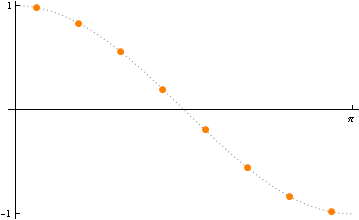
\includegraphics[width=0.4\textwidth]{Billeder/coskoefficienter.png}
\caption{Koefficienterne for $T(1,\ 1)$ og $f(0,\ y)$ afmærket som punkter på en cosinusbølge.}
\label{fig:cosko}
\end{figure}

Det ses desuden på figur \vref{fig:cosko}, at koefficienterne tilsammen har sum lig nul. Der er altså lige mange positive og negative koefficienter i alle bølgerne med undtagelse af den første, som udelukkende består af koefficienten $\frac{\sqrt{2}}{2}$.\\
At hele den første række kun indeholder positive indgange bidrager til energikomprimeringen. Hvis A indeholder lignende værdier, vil indgang $(0,\phantom{i}0)$ have stor numerisk værdi efter transformationen. Derfor kan en stor del af informationerne koncentreres i denne ene indgang. På samme måde vil resultatet af at prikke en vektor med ens indgange, $\vec{v}= \begin{bmatrix} v_1 & v_1 & \hdots & v_1 \end{bmatrix}$ med en hvilken som helst samling af koefficenter fra en cosinusbølge beregnet ved $i=0,\ldots,7$ blive lig nul. Resultatet af at prikke en vektor, med indgange der næsten er ens med koefficienterne, vil blive tæt på eller lig nul [\citet{whydomath_dct}, afsnit 4]

Koefficienten i indgang $(0,\phantom{i}0)$ omtales som DC koefficienten eller Direct Current. De resterende 63 koefficienter kaldes for AC koefficienter eller Alternating Current. Navnene stammer fra transformationens historiske brug i analyse af elektriske kredsløb og refererer til basisfunktionerne i transformationen, som for DC koefficienten er konstant som jævnstrøm, men de oscillerer som vekselstrøm for de resterende koefficienter [\citet{lokminglui_DCT}, s. 5].

De transformerede koefficienter udtrykker bestemte mønstre i signalet. Mønstrene for hver koefficient ses i figur \vref{fig:frekvens_matrix}, hvor bølgetoppene og -dalene i cosinusfunktionerne (og dermed negative og positive koefficienter) er henholdsvis sorte og hvide. Denne figur illustrerer hvordan transformationen behandler forskellige slags mønstre i signalet - mønstre som ligner signalet vil have høje koefficienter. Bemærk at DC koefficienten er en koefficient for et ensfarvet mønster eller signal.
\begin{figure}[htbp]
\centering

\includegraphics[width=0.35\textwidth]{billeder/frekvensmatrix.png}
\caption{Repræsentation af de 64 forskellige basisfunktioner i cosinustransformationen af længde $n = 8$. Mønstrene hører til koefficienterne, som fås ved transformation af et signal. Koefficienternes størrelse fortæller hvor meget, det tilhørende mønster optræder i signalet.}
\label{fig:frekvens_matrix}
\end{figure}
Indgangene i den transformerede matrix er koefficienterne, hvorved disse mønstre er repræsenteret i signalet. Altså kan signalet genskabes ved en lineær kombination af disse mønstre.

I dette projekt udføres beregninger og dermed også transformationen i Python. Til dette er det beregningsmæssigt nemmere og hurtigere at regne med DCT på matrixform.

I udledningen af DCT i appendiks \vref{DCT_udledning} ses formlen for den todimensionelle DCT, hvor ligning \vref{eq:soejlevektor} viser, hvordan hver enkelt søjle i en matrix for en n-punkts DCT beregnes. Da der i denne opgave regnes med matricer af størrelsen $8 \times 8$, vises der i ligning \ref{eq:DCTmatrix} en matrix beregnet ved $n=8$ - altså en $8 \times 8$-matrix.
%\begin{align}
%	y_{(i,j)} = C(i) \sqrt{\frac{2}{n}} \cos\left(\frac{(2 \cdot j-1) \cdot (i-1)\pi}{2n}\right)
%\label{eq:DCTmatrixform}
%\end{align}
%Hvor
%\begin{itemize}
%		\item{$C(i)= \begin{cases}
%			\frac{1}{\sqrt{2}} \ hvis \ i = 1\\
%			1\ \ \ hvis \ i \neq 1
%		\end{cases}
%		$}
%		\item{$y_{(i,j)}=$ indgang $(i,j)$}
%		\item{$n =$ matricens dimensioner n$\times$n}
%\end{itemize}
%Matricen beregnet ved formel \vref{eq:DCTmatrixform} hvor $n=8$ ses i ligning \ref{eq:DCTmatrix}.
\begin{equation}
U=\frac{1}{2}
\begin{bsmallmatrix}
	\frac{\sqrt{2}}{2}	& \frac{\sqrt{2}}{2}		& \frac{\sqrt{2}}{2}		& \frac{\sqrt{2}}{2}		& \frac{\sqrt{2}}{2}		& \frac{\sqrt{2}}{2}		& \frac{\sqrt{2}}{2}		& \frac{\sqrt{2}}{2}		\\
	\cos(\frac{\pi}{16})		& \cos(\frac{3\pi}{16})	& \cos(\frac{5\pi}{16})	& \cos(\frac{7\pi}{16})	& \cos(\frac{9\pi}{16})	& \cos(\frac{11\pi}{16})	& \cos(\frac{13\pi}{16})	& \cos(\frac{15\pi}{16})		\\
	\cos(\frac{2\pi}{16})	& \cos(\frac{6\pi}{16})	& \cos(\frac{10\pi}{16})	& \cos(\frac{14\pi}{16})	& \cos(\frac{18\pi}{16})	& \cos(\frac{22\pi}{16})	& \cos(\frac{26\pi}{16})	& \cos(\frac{30\pi}{16})		\\
	\cos(\frac{3\pi}{16})	& \cos(\frac{9\pi}{16})	& \cos(\frac{15\pi}{16})	& \cos(\frac{21\pi}{16})	& \cos(\frac{27\pi}{16})	& \cos(\frac{33\pi}{16})	& \cos(\frac{39\pi}{16})	& \cos(\frac{45\pi}{16})		\\
	\cos(\frac{4\pi}{16})	& \cos(\frac{12\pi}{16})	& \cos(\frac{20\pi}{16})	& \cos(\frac{28\pi}{16})	& \cos(\frac{36\pi}{16})	& \cos(\frac{44\pi}{16})	& \cos(\frac{52\pi}{16})	& \cos(\frac{60\pi}{16})		\\
	\cos(\frac{5\pi}{16})	& \cos(\frac{15\pi}{16})	& \cos(\frac{25\pi}{16})	& \cos(\frac{35\pi}{16})	& \cos(\frac{45\pi}{16})	& \cos(\frac{55\pi}{16})	& \cos(\frac{65\pi}{16})	& \cos(\frac{75\pi}{16})		\\
	\cos(\frac{6\pi}{16})	& \cos(\frac{18\pi}{16})	& \cos(\frac{30\pi}{16})	& \cos(\frac{42\pi}{16})	& \cos(\frac{54\pi}{16})	& \cos(\frac{66\pi}{16})	& \cos(\frac{78\pi}{16})	& \cos(\frac{90\pi}{16})		\\
	\cos(\frac{7\pi}{16})	& \cos(\frac{21\pi}{16})	& \cos(\frac{35\pi}{16})	& \cos(\frac{49\pi}{16})	& \cos(\frac{63\pi}{16})	& \cos(\frac{77\pi}{16})	& \cos(\frac{91\pi}{16})	& \cos(\frac{105\pi}{16})	\\
\end{bsmallmatrix}
\label{eq:DCTmatrix}
\end{equation}
Magen til ligning \vref{eq:DCTeq} kan $U$ bruges til at opnå DCT transformationen, blot hvor en stor del af udregningerne er udført på forhånd. På matrixform prikkes $U$ med $A$, og derefter prikkes dette resultat med $U^T$. Transformationen ses i ligning \vref{eq:DCTtrans}. %I beregningerne bruges den transponerede matrix, som ses i ligning \Vref{eq:DCTmatrixT}.
%\begin{equation}
%U^T = \frac{1}{2}
%\begin{bmatrix}
%\frac{2}{\sqrt{2}} & \cos(\frac{\pi}{16}) & \cos(\frac{2 \cdot \pi}{16}) & \cos(\frac{3 \cdot \pi}{16}) & \cos(\frac{4 \cdot \pi}{16}) & \cos(\frac{5 \cdot \pi}{16}) & \cos(\frac{6 \cdot \pi}{16}) & \cos(\frac{7 \cdot \pi}{16}) \\
%\frac{2}{\sqrt{2}} & \cos(\frac{3 \cdot \pi}{16}) & \cos(\frac{6 \cdot \pi}{16}) & \cos(\frac{9 \cdot \pi}{16}) & \cos(\frac{12 \cdot \pi}{16}) & \cos(\frac{15 \cdot \pi}{16}) & \cos(\frac{18 \cdot \pi}{16}) & \cos(\frac{21 \cdot \pi}{16}) \\
%\frac{2}{\sqrt{2}} & \cos(\frac{5 \cdot \pi}{16}) & \cos(\frac{10 \cdot \pi}{16}) & \cos(\frac{15 \cdot \pi}{16}) & \cos(\frac{20 \cdot \pi}{16}) & \cos(\frac{25\cdot \pi}{16}) & \cos(\frac{30 \cdot \pi}{16}) & \cos(\frac{35 \cdot \pi}{16}) \\
%\frac{2}{\sqrt{2}} & \cos(\frac{7 \cdot \pi}{16}) & \cos(\frac{14 \cdot \pi}{16}) & \cos(\frac{21 \cdot \pi}{16}) & \cos(\frac{28 \cdot \pi}{16}) & \cos(\frac{35 \cdot \pi}{16}) & \cos(\frac{42 \cdot \pi}{16}) & \cos(\frac{49 \cdot \pi}{16}) \\
%\frac{2}{\sqrt{2}} & \cos(\frac{9 \cdot \pi}{16}) & \cos(\frac{18 \cdot \pi}{16}) & \cos(\frac{27 \cdot \pi}{16}) & \cos(\frac{36 \cdot \pi}{16}) & \cos(\frac{45 \cdot \pi}{16}) & \cos(\frac{54 \cdot \pi}{16}) & \cos(\frac{63 \cdot \pi}{16}) \\
%\frac{2}{\sqrt{2}} & \cos(\frac{11 \cdot \pi}{16}) & \cos(\frac{22 \cdot \pi}{16}) & \cos(\frac{33 \cdot \pi}{16}) & \cos(\frac{44 \cdot \pi}{16}) & \cos(\frac{55 \cdot \pi}{16}) & \cos(\frac{66 \cdot \pi}{16}) & \cos(\frac{77 \cdot \pi}{16}) \\
%\frac{2}{\sqrt{2}} & \cos(\frac{13 \cdot \pi}{16}) & \cos(\frac{26 \cdot \pi}{16}) & \cos(\frac{39 \cdot \pi}{16}) & \cos(\frac{52 \cdot \pi}{16}) & \cos(\frac{65 \cdot \pi}{16}) & \cos(\frac{78 \cdot \pi}{16}) & \cos(\frac{91 \cdot \pi}{16}) \\
%\frac{2}{\sqrt{2}} & \cos(\frac{15 \cdot \pi}{16}) & \cos(\frac{30 \cdot \pi}{16}) & \cos(\frac{45 \cdot \pi}{16}) & \cos(\frac{60 \cdot \pi}{16}) & \cos(\frac{75 \cdot \pi}{16}) & \cos(\frac{90 \cdot \pi}{16}) & \cos(\frac{105 \cdot \pi}{16})
%\end{bmatrix}
%\label{eq:DCTmatrixT}
%\end{equation}
\begin{align}
B=U \cdot A \cdot U^T
\label{eq:DCTtrans}
\end{align}
Hvor
\begin{itemize}
	\item $B$: den transformerede matrix
	\item $U$: DCT-matricen
	\item $A$: $8\times8$ matrix af pixelværdier
\end{itemize}
Denne similærtransformation (similaritet forklares senere på side \pageref{sec:similaritet}) har samme effekt på $8\times8$-matricen som ligning \vref{eq:DCTeq}. Ligning \ref{eq:DCTtrans} kan skrives som en sammensat transformation bestående af to transformationer med henholdsvis $U$ og $U^T$ som standardmatricer. De to transformationer ses i ligning \ref{eq:trans1} og \ref{eq:trans2}.
\begin{align}
T(A)=U \cdot A
\label{eq:trans1}
\end{align}
\begin{align}
Q(A)=A \cdot U^T
\label{eq:trans2}
\end{align}
Den sammensatte transformation ser derfor ud som i ligning \ref{sammensat_transformation}.
\begin{align}
Q(T(A))=U \cdot A \cdot U^T=B
\label{sammensat_transformation}
\end{align}
Fremover refereres der til den transformerede matrix som $B$.
\subsubsection*{Ortonormalitet}\label{sec:ortonormalitet}
$U$ er en ortonormal matrix, hvilket ses i ligning \vref{eq:diff_delta}, hvilket er et specialtilfælde af en ortogonal matrix. For ortogonale matricer gælder, at
\begin{itemize}
	\item{alle ortogonale sæt af vektorer som ikke er nul er lineært uafhængige.}
	\item{vektorerne er ortogonale på hinanden.}
	\item{alle underrum i $\mathbb{R}^n$ indeholder en ortogonal basis.}
	\item{$Z^{-1} = Z^T$ [\citet{linalg}, s. 413].}
\end{itemize}
En ortonormal matrix er en ortogonal matrix, hvor der gælder, at søjlerne er vektorer med længden 1 [\citet{linalg}, s. 374].
\subsubsection*{Bijektivitet og invertibilitet}
Den diskrete cosinustransformation skal være invertibel, da det ellers ikke giver mening at transformere data til et kodomæne, hvorfra det ikke kan lade sig gøre at komme tilbage til domænet. En lineær transformation er kun invertibel, hvis den er bijektiv [\citet{linalg}, s. 555].

En lineær transformation $T:\mathbb{R}^n \longrightarrow \mathbb{R}^n$ med standardmatrix $A$ er invertibel, hvis og kun hvis $A$ er invertibel. I så fald er den inverse transformation $T^{-1}$ og dens standardmatrix er $A^{-1}$ [\citet{linalg}, s. 187].

En lineær transformation $T:\mathbb{R}^n \longrightarrow \mathbb{R}^m$ siges at være bijektiv, hvis den er både surjektiv og injektiv og derved bijektiv [\citet{linalg}, s. 555].

Altså ønskes det at vise, at den diskrete cosinustransformation er bijektiv.

\textbf{Surjektivitet}\\
En lineær transformation $T:\mathbb{R}^n \longrightarrow \mathbb{R}^m$ siges at være surjektiv, hvis transformationens billedmængde er lig kodomænet $\mathbb{R}^n$ [\citet{linalg}, s. 180].

For en surjektiv lineær transformation $T:\mathbb{R}^n \longrightarrow \mathbb{R}^m$ med standardmatrix $A$ gælder, at
\begin{align}
Rank(A)	&	=m\\
Col(A)	&	=\mathbb{R}^m
\end{align} [\citet{linalg}, s. 181]

Da matricen $U$, som er standardmatrix i cosinustransformationen, opfylder de to ovenstående krav på baggrund af, at den er ortonormal og kvadratisk, kan der sluttes, at den lineære transformation med standardmatrix $U$ er surjektiv.

\textbf{Injektivitet}\\
En lineær transformation $T:\mathbb{R}^n \longrightarrow \mathbb{R}^m$ siges at være injektiv, hvis hvert par af særskilte vektorer i domænet $\mathbb{R}^n$ har særskilte billeder i kodomænet $\mathbb{R}^m$ [\citet{linalg}, s. 182].

For en injektiv lineær transformation $T:\mathbb{R}^n \longrightarrow \mathbb{R}^m$ med standardmatrix $A$ gælder, at
\begin{align}
Null(A)	&	=0\\
Rank(A)	&	=n
\end{align} [\citet{linalg}, s. 184]

Da matricen $U$ opfylder de to ovenstående krav på baggrund af, at den er ortonormal og kvadratisk, kan der sluttes, at den lineære transformation med standardmatrix $U$ er injektiv.

Da den lineære transformation med standardmatrix $U$ er både injektiv og surjektiv, er den altså bijektiv. Disse egenskaber gør, at transformationen kan inverteres, som vist i ligning \ref{eq:similaere2}.
\subsubsection*{Similaritet}\label{sec:similaritet}
Som tidligere nævnt er udtryk \ref{eq:DCTtrans} en similærtransformation, og defintionen for similaritet lyder som følgende: To kvadratiske matricer, $A$ og $B$, siges at være similære, hvis der findes en invertibel matrix, $P$, som opfylder
\begin{align}
B=P^{-1} \cdot A \cdot P
\end{align}
Da der gælder at $U^T=U^{-1}$ [\citet{linalg}, s. 413] sluttes, at ligningerne \ref{eq:similaere1} og \ref{eq:similaere2} gælder.
\begin{align}
B = U \cdot A \cdot U^{-1} = U \cdot A \cdot U^T
\label{eq:similaere1}
\end{align}
\begin{align}
A = U^{-1} \cdot B \cdot U = U^T \cdot B \cdot U
\label{eq:similaere2}
\end{align}
Matricerne $A$ og $B$ er altså similære matricer. Transformationen er dermed en similærtransformation \citep{similar_wolfram}. Den diskrete cosinus transformation ses også som værende invertibel ved
\begin{align}
B=U \cdot A \cdot U^T
\end{align}
Da $A$ og $B$ er similære, er transformationen et basisskift da følgende ligning gælder.
\begin{align}
B=P^{-1} \cdot A \cdot P
\end{align}
Hvor
\begin{itemize}
	\item{$A$: $n \times n$-matrix}
	\item{$B$: $n \times n$-matrix}
	\item{$P$: $U^T$}
\end{itemize}
$B$ er altså $A$ udtrykt i basen $U^T$. Basisskiftet gør det nemmere at foretage den tidligere omtalte udvælgelse af vigtige informationer

Hermed er der redegjort for DCT og dens egenskaber, og der bliver i næste sektion vist eksempler på transformation af diverse $8\times8$-matricer, før den videre algoritme forklares.
%Den diskrete cosinus transformation er ydermere invertibel, og den inverse transformation kan let udledes fra transformationen i ligning \vref{eq:DCTtrans} \citep{whydomath_dct}. For at nå frem til den inverse transform benyttes den associative lov om matrixmultiplikation \citep{linalg}.
%\begin{align}
%A \cdot (C \cdot P)=(A \cdot C) \cdot P
%\end{align}
%for matrixdimensioner
%\begin{itemize}
%	\item{$A=k \times m$}
%	\item{$C=m \times n$}
%	\item{$P=n \times p$}
%\end{itemize}
%Med denne regneregel kan den inverse transformation udledes.
%\begin{align}
%A
%\ =I_n \cdot A \cdot I_n
%\ = (U^T \cdot U) \cdot A \cdot (U^T \cdot U)
%\end{align}
%Den associative lov om matrixmultiplikation benyttes.
%\begin{align}
%A=U^T \cdot (U \cdot A \cdot U^T) \cdot U
%\end{align}
%Det ses at udtrykket i parentesen er magen til udtrykket i ligning \vref{eq:DCTtrans}.
%\begin{align}
%A=U^T \cdot B \cdot U
%\label{eq:DCTinvers}
%\end{align}
%Det ses altså at transformationen i ligning \ref{eq:DCTtrans} kan inverteres ved ligning \ref{eq:DCTinvers}.
\subsection{Eksempler på brug af den diskrete cosinustransformation}
For at illustrere hvordan den diskrete cosinustransformation fungerer, vises her eksempler på $8\times8$ matricer transformeret ved den diskrete cosinustransformation. Da billeder er det, der undersøges i dette projekt, vises de respektive $8\times8$ billeder tilhørende matricerne også. Der er trukket 128 fra alle indgange inden transformationen, hvilket bl.a. forsimpler processen med kvantisering - dette uddybes i afsnit \ref{sec:preprocessing}. Alle koefficienter er desuden afrundet til nærmeste heltal efter transformationen, for at gøre matricerne letlæselige. Der gøres opmærksom på, at der kan være koefficienter, som bliver afrundet til nul. Alle koeffiecienter, som er nul, repræsenteres af ".".
\begin{figure}[htbp]
\centering

\includegraphics[width=0.15\textwidth]{Billeder/8x8_eks1.png}
\caption{$8 \times 8$ billede som består udelukkende af pixels med intensitet 100.\label{fig:8x8graa}}
\end{figure}

\begin{figure}[htbp]
\begin{minipage}[b]{0.45\linewidth}
\centering
$\begin{bmatrix}
100	&	100	&	100	&	100	&	100	&	100	&	100	&	100\\
100	&	100	&	100	&	100	&	100	&	100	&	100	&	100\\
100	&	100	&	100	&	100	&	100	&	100	&	100	&	100\\
100	&	100	&	100	&	100	&	100	&	100	&	100	&	100\\
100	&	100	&	100	&	100	&	100	&	100	&	100	&	100\\
100	&	100	&	100	&	100	&	100	&	100	&	100	&	100\\
100	&	100	&	100	&	100	&	100	&	100	&	100	&	100\\
100	&	100	&	100	&	100	&	100	&	100	&	100	&	100
\end{bmatrix}$
\caption{Pixelværdier for figur \ref{fig:8x8graa}.\label{fig:graamatrix}}
\end{minipage}
\hspace{1.0cm}
\begin{minipage}[b]{0.45\linewidth}
\centering
$\begin{bmatrix}
-224		&	.	&	.	&	.	&	.	&	.	&	.	&	.\\
.		&	.	&	.	&	.	&	.	&	.	&	.	&	.\\
.		&	.	&	.	&	.	&	.	&	.	&	.	&	.\\
.		&	.	&	.	&	.	&	.	&	.	&	.	&	.\\
.		&	.	&	.	&	.	&	.	&	.	&	.	&	.\\
.		&	.	&	.	&	.	&	.	&	.	&	.	&	.\\
.		&	.	&	.	&	.	&	.	&	.	&	.	&	.\\
.		&	.	&	.	&	.	&	.	&	.	&	.	&	.\\
\end{bmatrix}
$
\caption{Figur \ref{fig:graamatrix} transformeret.\label{fig:trans_matrix1}}
\end{minipage}
\end{figure}
I figur \ref{fig:graamatrix} har alle indgange en værdi på 100, hvilket svarer til et billede bestående af 64 pixels i samme gråtone med farveintensitet på 100. I figur \ref{fig:8x8graa} ses matricen repræsenteret ved et billede, og i figur \ref{fig:trans_matrix1} ses den transformerede matrix. Det ses at alle koefficienter er lig nul med undtagelse af DC koefficienten, som er lig -224. Altså kan hele det behandlede signal udtrykkes ved indgang $(0, 0)$, da det kun er den første basisfunktion, som bruges til at repræsentere billedet.

I figur \ref{fig:tern_matrix} udtrykkes matricen for et billede, som består af 64 pixels, hvoraf halvdelen er i gråtoner med farveintensitet = 100, og den anden halvdel er hvide med farveintensitet = 255. Det ses i \ref{fig:trans_matrix2}, at koefficienterne er anderledes end i \ref{fig:trans_matrix1} og udtrykker signalet ved andre koefficienter. Denne gang benyttes flere AC koefficienter for at udtrykke signalet, da der er mere variation i signalet.
\begin{figure}[htbp]
\centering

\includegraphics[width=0.15\textwidth]{Billeder/8x8_eks3.png}
\caption{$8 \times 8$ billede bestående af grå og hvide pixels med farveintensiteter på henholdsvis 100 og 255.}
\label{fig:8x8halvgraa}
\end{figure}
\begin{figure}[htbp]
\begin{minipage}[b]{0.45\linewidth}
\centering
$\begin{bmatrix}
100	&	100	&	100	&	100	&	255	&	255	&	255	&	255\\
100	&	100	&	100	&	100	&	255	&	255	&	255	&	255\\
100	&	100	&	100	&	100	&	255	&	255	&	255	&	255\\
100	&	100	&	100	&	100	&	255	&	255	&	255	&	255\\
255	&	255	&	255	&	255	&	100	&	100	&	100	&	100\\
255	&	255 &	255	&	255	&	100	&	100	&	100	&	100\\
255	&	255	&	255	&	255	&	100	&	100	&	100	&	100\\
255	&	255	&	255	&	255	&	100	&	100	&	100	&	100
\end{bmatrix}$
\caption{Pixelværdier for figur \ref{fig:8x8halvgraa}.\label{fig:tern_matrix}}
\end{minipage}
\hspace{1.0cm}
\begin{minipage}[b]{0.45\linewidth}
\centering
$\begin{bmatrix}
396	&	.		&	.	&	.	&	.	&	.	&	.	&	.	\\
.	&	-509		&	.	&	179	&	.	&	119	&	.	&	101	\\
.	&	.		&	.	&	.	&	.	&	.	&	.	&	.	\\
.	&	179		&	.	&	-63	&	.	&	42	&	.	&	-36	\\
.	&	.		&	.	&	.	&	.	&	.	&	.	&	.	\\
.	&	-119		&	.	&	42	&	.	&	-28	&	.	&	24	\\
.	&	.		&	.	&	.	&	.	&	.	&	.	&	.	\\
.	&	101		&	.	&	-36	&	.	&	24	&	.	&	-20
\end{bmatrix}
$
\caption{Figur \ref{fig:tern_matrix} transformeret.\label{fig:trans_matrix2}}
\end{minipage}
\end{figure}
Matricen i figur \ref{fig:trans_matrix2} viser, at når et billede har store og bratte ændringer mellem farveintensiteter, skal der bruges mange cosinusfunktioner til at udtrykke det bratte skift i farveintensitet. Dette er de tilfælde, som cosinusfunktionen ikke behandler godt - der opnås ikke god energikomprimering.

I figur \ref{fig:gradient_matrix} ses en matrix, som laver en glat overgang fra hvid til sort i samme mønster som den i figur \ref{fig:tern_matrix}. Denne glatte overgang skulle gerne være lettere for cosinusfunktionen at energikomprimere, da der ikke sker bratte skift i farveintensitet. Det tilsvarende billede ses i figur \ref{fig:gradient} og den transformerede matrix ses i figur \ref{fig:trans_matrix3}. Af den transformerede matrix ses det, at cosinustransformationen har haft lettere ved at energikomprimere denne matrix end den i figur \ref{fig:tern_matrix}. Det antages, at billeder primært har glatte overgange mellem farveintensiteter, som ligner den i figur \ref{fig:gradient}.
\begin{figure}[htbp]
\centering

\includegraphics[width=0.15\textwidth]{Billeder/8x8_eks6.png}
\caption{$8\times8$ billede bestående af pixels med gradvis overgang fra hvid til sort.}
\label{fig:gradient}
\end{figure}
\begin{figure}[htbp]
\begin{minipage}[b]{0.45\linewidth}
\centering
$\begin{bmatrix}
255	&	236	&	200	&	153	&	102	&	55	&	19	&	0\\
236	&	236	&	200	&	153	&	102	&	55	&	19	&	19\\
200	&	200	&	200	&	153	&	102	&	55	&	55	&	55\\
153	&	153	&	153	&	153	&	102	&	102	&	102	&	102\\
102	&	102	&	102	&	102	&	153	&	153	&	153	&	153\\
55	&	55	&	55	&	102	&	153	&	200	&	200	&	200\\
19	&	19	&	55	&	102	&	153	&	200	&	236	&	236\\
0	&	19	&	55	&	102	&	153	&	200	&	236	&	255
\end{bmatrix}$
\caption{Pixelværdier til figur \ref{fig:gradient}.\label{fig:gradient_matrix}}
\end{minipage}
\hspace{1.0cm}
\begin{minipage}[b]{0.45\linewidth}
\centering
$\begin{bmatrix}
-4	&	.	&	.	&	.	&	.	&	.	&	.	&	.	\\
.	&	568	&	.	&	-40	&	.	&	-4	&	.	&	-1	\\
.	&	.	&	.	&	.	&	.	&	.	&	.	&	.	\\
.	&	-40	&	.	&	54	&	.	&	-11	&	.	&	-1	\\
.	&	.	&	.	&	.	&	.	&	.	&	.	&	.	\\
.	&	-4	&	.	&	-11	&	.	&	24	&	.	&	-5	\\
.	&	.	&	.	&	.	&	.	&	.	&	.	&	.	\\
.	&	-1	&	.	&	-1	&	.	&	-5	&	.	&	22
\end{bmatrix}$
\caption{Figur \ref{fig:gradient_matrix} transformeret.\label{fig:trans_matrix3}}
\end{minipage}
\end{figure}
Den inverse transformation producerer de to originale matricer uden afvigelser. Skridtet er inverterbart og uden tab af informationer.

Opsummeres ovenstående afsnit om DCT er de vigtigste pointer at
\begin{itemize}
\item[...] DCT transformerer fra tidsdomænet til frekvensdomænet
\item[...] DCT på matrixform er udtrykt ved ligningen $B=U \cdot A \cdot U^T$, hvor $U$ er udtrykt ved ligning \vref{eq:DCTtrans}
\item[...] den inverse DCT er udtrykt som $A = U^T \cdot B \cdot U$ 
\end{itemize}

Med DCT-transformationens egenskaber i mente, ses der nu på de resterende elementer i JPEG-komprimeringen. 
\subsection{Forbehandling af billede} \label{sec:preprocessing}
Før billedet transformeres med den diskrete cosinustransformation, skal det forbehandles. Dette indebærer at dele billedet op i undermatricer af $8\times8$ pixels - kvadratiske matricer med 64 indgange. Størrelsen af disse undermatricer af pixels er ikke tilfældig, og har udgangspunkt i egenskaberne ved den diskrete cosinustransformation. Som forklaret i afsnit \vref{sec:teori_intro} antages det, at nærliggende pixels i et billede er korrelerede, og at ikke-nærliggende pixels ikke er korrelerede. Dermed er det formålsløst at forsøge at transformere et helt billede, i håb om at kunne energikomprimere dette. Derfor deles billedet op i mindre undermatricer, og disse transformeres enkeltvis. Den optimale størrelse af disse undermatricer er $8 \times 8$ pixels, hvilket der er flere grunde til.

Matricer af $2\times2$ pixels indeholder ikke nok data for DCT at bearbejde med, og når transformationen skal udtrykke matricen som funktioner af cosinusbølger, er der ikke nok cosinusbølger til at kunne udtrykke matricen til billedet præcist - der er nemlig kun fire. Resultatet er, at datarepræsentationen er upræcist, og at billedet mister for meget kvalitet - det kan ses med det menneskelige øje. Dette skyldes transformationens høje energikomprimering [\citet{guillermo_sapiro}, 19:26-23:52]. Matricer af $4\times4$ lider under tilsvarende problem som $2\times2$ dog i mindre grad.\\
Matricer af $8\times8$ pixels har en størrelse, der gør cosinustransformationen effektiv. Der er nok indgange og dermed cosinusfunktioner til at kunne udtrykke matricen præcist. Desuden kræver energikomprimeringen, at flere pixels kan repræsenteres af enkelte værdier, og det er derfor vigtigt, at de nærliggende pixels ligner hinanden. Hvis dette er tilfældet, hvilket det ofte er i $8 \times 8$ matricer, kan matricen komprimeres. Altså er der nok cosinusfunktioner og nok korrelation mellem de enkelte pixels til, at $8 \times 8$ er en fornuftig størrelse [\citet{guillermo_sapiro}, 19:26-23:52].\\
Årsagerne til ikke at bruge større end $8 \times 8$, som eksempelvis $16\times16$, er flere; det er beregningsmæssigt langt mere effektivt at udføre komprimeringen på mindre matricer - en computer skal bruge færre beregninger, komprimeringsalgoritmen fungerer ud fra princippet om, at nærliggende pixels ligner hinanden, hvilket er mere usandsynligt ved $16 \times 16$ end $8 \times 8$. Cosinustransformationens energikomprimering fungerer bedst, når der er korrelation mellem de pixels, som transformeres - så kan flere pixels udtrykkes ved få værdier i frekvensdomænet. Problemet med at bruge større matricer end $8\times8$ er, at der ikke nødvendigvis er nogen korrelation mellem de enkelte pixels i en stor matrix. Det bliver meget mere sandsynligt, at billedet tydeligt skifter farve over et stort område, og det giver derfor ikke mening at prøve at sammenligne disse pixels, da der sandsyndligvis ikke er nogen korrelation mellem dem [\citet{guillermo_sapiro}, 21:16-21:52].\\
Altså transformeres kun matricer af størrelse $8\times8$ af gangen. Disse kvadratiske matricer af billedet, kaldes som tidligere nævnt $A$. Figur \vref{fig:pixelblok} viser et eksempel på en $8 \times 8$ pixelmatrix. Bemærk at denne matrix kun består af pixels i gråtoner.

Billeder i gråtoner kan deles op som i figur \vref{fig:pixelblok}, og billeder i RGB-farveformatet beskrives med én værdi for hver farve i hver pixel - altså tre værdier. Billeder i farver deles op i de tre farverum, og de enkelte farverum bearbejdes på samme måde som ved gråtoner. Efterfølgende sammensættes de tre farverum igen for at danne billedet.
Hvert farverum opdeles i $A$-matricer, og der subtraheres 128 fra samtlige indgange. Dette gøres for at ændre værdierne fra beliggende i intervallet $[0;255]$ til $[-128;127]$ og dermed centrere dem omkring nul. Dette er ønskværdigt for komprimeringen, da kvantiseringsskridtet dermed efter cosinustransformationen formår at skabe flere ens koefficienter, hvilket gør komprimeringen mere effektiv, men dette uddybes senere.\\
Såfremt billedets dimensioner (både højde og bredde) ikke går op i otte, fyldes de ufuldendte $8 \times 8$ matricer ud med nuller. Dette hedder nulfyldning [\citet{zero_padding}, s. 1]. Nulfyldning er nødvendigt, da DCT i denne rapport bruges på matricer af størrelse $8\times8$, og billedet vil ikke altid have dimensioner, som 8 ikke går op i. Dette resulterer dog i, at der indsættes en grå kant på billedet, som kan give en kontrast til det originale billede, hvilket betyder, at der formentlig opstår større unøjagtigheder i kanten af billedet. Dette har indflydelse på transformationen og dermed hele komprimeringsalgoritmen. Der nøjes dog med at påpege problemet, men ikke lave en bedre løsning end nulfyldning. Det er i det hele taget et grundlæggende problem ved DCT, at transformationen ikke behandler store skift i farveintensitet godt, da den forsøger at udtrykke glatte overgange. Hvis der ikke er glatte overgange, fungerer energikomprimeringen ringe.

Efter forbehandlingen fås en samling af undermatricer bestående af 64 pixels hver, og som tilsammen udgør det komplette billede. Dermed er billedet klar til cosinustransformationen fra forrige sektion.

Ønskes det at invertere forbehandlingsskridtet, skal der indgangsvist adderes med 128 på alle indgange, og det opsplittede billede skal samles fra $8 \times 8$ matricerne til det samlede billede igen. Forbehandlingsskridtet er herved inverteret, hvilket gøres uden tab eller forandringer i dataene.
\subsection{Kvantisering}\label{sec:kvantisering}
Tredje skridt i komprimeringsalgoritmen omhandler kvantisering af de transformerede værdier. Kvantiseringen har til formål at smide de overflødige data væk og desuden gøre billedet klar til fjerde og sidste skridt. Med overflødig data menes der informationer om billedet, som ikke har nogen (eller lille) synlig indflydelse på billedkvaliteten. Da DCT-transformationen har energikomprimeret $A$, repræsenterer de mindste koefficienter de data, der fremkommer mindst i matricen. Da det menneskelige øje har svært ved at se meget hurtige ændringer i farveintensitet over små afstande, er høje frekvensændringer ikke tydelige for det menneskelige øje. Altså er koefficienterne, i nedre højre hjørne af $B$, ikke betydningsfulde for opfattelsen af billedet som helhed.

Kvantiseringen gør brug af indgangsvis division med en $8 \times 8$ matrix (indgang $B_{1,\phantom{i}1}$ divideres med indgang $Q_{1,\phantom{i}1}$ osv.). Denne matrix består af heltal, som  er bestemt empirisk ved eksperimenter omhandlende det menneskelige syn. Tallene i matricen er tilpasset således, at den synlige billedkvalitet er høj, mens billedet komprimeres mest muligt [\citet{lokminglui}, s. 4]. Der findes flere forskellige kvantiseringsmatricer, og den der bruges i dette projekt, er den som bruges i JPEG-standarden [\citet{lokminglui}, s. 4]. Kvantiseringsmatricen, som fremover refereres til som $Q$, ses i ligning \ref{eq:Q50teori}.
\begin{equation}
Q50 =
\begin{bmatrix}
	16	&	11	& 10		& 16		& 	24	&	40	& 51		& 61		\\
	12	&	12	& 14		& 19		& 	26	& 	58	& 60		& 50		\\
	14	&	13	& 16		& 24		& 	40	& 	57	& 69		& 56		\\
	14	&	17	& 22		& 29		& 	51	& 	87	& 80		& 62		\\
	18	&	22	& 37		& 56		& 	68	& 	109	& 103	& 77		\\
	24	&	35	& 55		& 64		& 	81	& 	104	& 113	& 92		\\
	49	&	64	& 78		& 87		& 	103	& 	121	& 120	& 101	\\
	72	&	92	& 95		& 98		& 	112	& 	100	& 103	& 99		\\
\end{bmatrix}
\label{eq:Q50teori}
\end{equation}
Matricen i ligning \vref{eq:Q50teori} hedder $Q50$, fordi den er kvantiseringsmatricen for en komprimering med kvalitet 50 (fremover benævnes Q-værdien blot som eksempelvis $Q50$ eller $Q10$ ved de respektive kvaliteter). I JPEG kan komprimeringsgraden justeres, og det er med denne matrix dette gøres. Matricen kan have en kvalitet mellem 1 og 100, hvor 100 resulterer i laveste komprimering og højeste billedkvalitet, mens 1 omvendt resulterer i højeste komprimering og laveste billedkvalitet. Det er værd at bemærke at $Q50$ ikke komprimerer et billede med 50\% eller 50 gange - værdien er blot et udtryk for en position på en skala fra 1 til 100.\\
For at opnå en anden kvalitet end 50, ændres Q med en bestemt formel. Alt efter den ønskede kvalitet gælder to formler, som begge multiplicerer hver enkelt indgang med en konstant, der beregnes på baggrund af den ønskede kvalitet.
\begin{align}
Q_n=\begin{cases}
	\frac{100-n}{50} \cdot Q50 \ hvis \ n > 50\\
	\frac{50}{n} \cdot Q50 \ \ \ \ \ hvis \ n < 50
\end{cases}
\end{align}
Herunder ses en kvantiseringsmatrix til en kvalitet på 25.
\begin{equation}
Q25 =
\begin{bmatrix}
	32	&	22	& 20		& 32		& 	48	&	80	& 102	& 122	\\
	24	&	24	& 28		& 38		& 	52	& 	116	& 120	& 100	\\
	28	&	26	& 32		& 48		& 	80	& 	114	& 138	& 112	\\
	28	&	34	& 44		& 58		& 	102	& 	174	& 160	& 124	\\
	36	&	44	& 74		& 112	& 	136	& 	218	& 206	& 134	\\
	48	&	70	& 110	& 128	& 	162	& 	208	& 226	& 184	\\
	98	&	128	& 156	& 174	& 	206	& 	242	& 240	& 202	\\
	144	&	184	& 190	& 196	& 	224	& 	200	& 206	& 198	\\
\end{bmatrix}
\label{eq:Q25teori}
\end{equation}
Matricen B kvantiseres ved indgangsvis division med Q.
\begin{align}
C_{(i,\ j)}=\frac{B_{(i,\ j)}}{Q50_{(i,\ j)}}
\label{C_beregning}
\end{align}
Indgangene i $B$ afrundes til nærmeste heltal, og matricen er dermed kvantiseret. Den kvantiserede matrix navngives $C$. Afrundingen gør at komprimeringen mister data, hvilket er et uigenkaldeligt tab af data og kan altså ikke gøres om. Når den komprimerede fil dekomprimeres til et billede, kan det originale billede ikke genskabes, da det inverterede kvantiseringsskridt vil resultere i andre værdier end det originale input, da afrundingen "sletter"\ dataene. Brugen af en ikke-tabsfri komprimering retfærdiggøres ved at de data, som smides væk, ikke har stor betydning for billedets generelle udseende - det menneskelige øje opfatter ikke tydeligt de manglende værdier, når billedet igen dekomprimeres. Desuden gør dette skridt den senere tabsfri komprimering med Huffman væsentligt mere effektiv.

Det ses på $Q$, at indgangene i nederste højre hjørne er væsentligt højere end indgangene i øverste venstre hjørne. Dette resulterer i, at værdier i nederste højre hjørne af $B$ bliver divideret med større tal end i øvre venstre hjørne. Dette betyder imidlertid, at der er større chance for, at tal i nedre højre hjørne bliver afrundet til heltal tæt på eller lig nul, og at værdier i øverste venstre hjørne vil forblive høje i forhold til de øvrige værdier. De mange værdier tæt på eller lig nul skyldes den tidligere centrering omkring nul, da der blev trukket 128 fra alle indgange i $A$. Altså vil $C$ hovedsageligt bestå af nuller og nogle få indgange i øverste venstre hjørne, som ikke er nul.
					
Det ses også, at en højere komprimeringsgrad resulterer i højere heltal i $Q$. Dette gør, at $C$ vil bestå af endnu lavere værdier, og flere vil blive afrundet til nul. Altså vil en endnu større mængde data gå tabt, og billedkvaliteten vil tilsvarende falde. Modsat vil en lavere komprimering resultere i lavere heltal i $Q$ og højere tal i $C$ med færre værdier afrundet til nul. Filen vil i dette tilfælde ende med at fylde mere, men med højere billedkvalitet.

Når dette skridt skal inverteres, ganges $C$ indgangsvis med $Q$-matricen, som blev brugt under komprimeringen.
\begin{align}
B_{(i,\ j)}=C_{(i,\ j)} \cdot Q_{(i,\ j)}
\end{align}
Det er nødvendigt at matricen $Q$, som bruges til inverteringen af skridtet, er magen til den som blev brugt under kvantiseringen. Hvis dette ikke gøres korrekt, vil det lede til værdier i $B$, som ikke ligner de originale, da der ganges med andre tal, end der oprindeligt blev divideret med.

I ligning \ref{fig:kvantiseret} ses et eksempel på en kvantiseret matrix. Matricen som kvantiseres er den fra figur \vref{fig:graamatrix}, og den kvantiseres med $Q50$.
\begin{equation}\resizebox{0.25\textwidth}{!}{$
	C=
\begin{bmatrix}
	2	&	.	& .		& .		& 	.	&	.	& .		& .	\\
	.	&	4	& .		& .		& 	.	& 	.	& .		& .	\\
	.	&	.	& .		& .		& 	.	& 	.	& .		& .	\\
	.	&	1	& .		& .		& 	.	& 	.	& .		& .	\\
	.	&	.	& .		& .		& 	.	& 	.	& .		& .	\\
	.	&	.	& .		& .		& 	.	& 	.	& .		& .	\\
	.	&	.	& .		& .		& 	.	& 	.	& .		& .	\\
	.	&	.	& .		& .		& 	.	& 	.	& .		& .	\\
\end{bmatrix}$}
\label{fig:kvantiseret}
\end{equation}
Her ses det, at mange af koefficienterne er blevet afrundet til nul, og de som ikke er afrundet til nul, er blevet små tal, hvorved matricen er blevet kvantiseret.
\subsection{Entropikodning - Huffmankodning}
\label{sec:Huffman}
Entropikodning som emne vil ikke blive uddybet her, men blot anses som en metode til at definere sandsynligheden af et givent datasæts udkom og repræsentere dette på bedste vis. Der findes flere forskellige entropikodnings-metoder, bl.a. Zigzag- og Huffmankodning. I denne rapport undersøges Huffmankodning. Enkelte grundelementer i grafteori vil dog blive præsenteret, da disse er nødvendige for at forstå Huffmankodning.

Huffmankodning fungerer vha. grafteori, og de nødvendige begreber er [\citet{grafteori}, s. 1-2]:
\begin{itemize}
\item En \emph{knude} er en samling af kanter
\item En \emph{kant} er en forbindelse mellem knuder
\item \emph{Valens} er antallet af kanter, der støder op til en knude
\item Et \emph{blad} er et knude med valens én
\item En \emph{graf} består af knuder og kanter
\item Et \emph{træ} er en sammenhængende graf
\item Et \emph{undertræ} er et afsnit af træet
\item \emph{Sti} er en forbindelse mellem to knuder, hvor alle knuder på stien er forskellige
\end{itemize}
Huffmankodning er en slags entropikodning og er en tabsfri komprimeringsmetode, hvorpå en stor mængde data kan repræsenteres ved hjælp af de enkelte symbolers (i dette tilfælde tallene $0-255$) sandsynlighed for at fremkomme. Komprimering med Huffmankodning tildeler alle symboler, der fremkommer i datastrengen, en bitrepræsentation af variabel længde, der afhænger af symbolets sandsynlighed. Dette betyder at et symbol, der fremkommer mange gange vil være tildelt et kortere kodeord end et symbol, der fremkommer få gange. Herved vil mængden af bits brugt til at repræsentere en datastreng blive nedbragt, da symboler der fremkommer mange gange fylder mindre, end dem der fremkommer få gange. Et kodeord er en binær repræsentation af symbolet og kunne eksempelvis være
\begin{align}
"A: 0, B: 10, C: 110, D: 111"
\label{fx:huffman prefix}
\end{align}
Vigtigt at nævne er, at Huffmankodning er en præfix-fri kode, hvilket betyder, at symboler ikke kan beskrives som sammensætning af andre symboler. Havde eksempel \vref{fx:huffman prefix} været $"A: 0, B: 1, C: 10, D: 11"$, ville en streng af $0$ og $1$ ikke kunne afkodes uden, at kodeordene var synligt adskilt, da det ikke vil være muligt, at se om $10$ betyder B, A eller C. Det er derfor vigtigt i Huffmankodning, at der ikke er nogle præfix for symbolerne, men at koden kan interpreteres entydigt.
\subsubsection{Huffmantræ} \label{sec:huffmanteori}
Huffmankodning foregår vha. skabelsen af et Huffmantræ, som er et overblik over sandsynligheden for, at de enkelte symboler fremkommer, og hvilket kodeord de skal tildeles. Kodeordet er stien ned til bladet. For at forklare skabelsen af et Huffmantræ laves et eksempel bestående af fire symboler, der viser principperne i skabelsen af træet.
Lad os antage at datastrengen lyder $$ abbacdababaccaddabbbacaadabaaddaaccaaaadaadaabaadacaadabaaadacaaadabaa $$ så kan sandsynligheden for at de enkelte symboler fremkomst i datastrengen beregnes. Disse er angivet i tabel \ref{tb:huffman_sandsynlighed}.

Ud fra tabel \vref{tb:huffman_sandsynlighed} opstilles der fire blade med hvert deres symbol som indgang, se figur \vref{fig:huffmantrae_ex1}. Herefter opstilles de to blade med den mindste sandsynlighed i et undertræ med bladene som indgange, se figur \vref{fig:huffmantrae_ex2}. I dette eksempel vil det være bladene for b og c, hvor bladet med mindst sandsynlighed placeres yderst til højre. Hyppigheden af dette undertræ er summen af de to blades sandsynlighed og giver her $0,11+0,16=0,27$. Derudover tildeles kanterne hhv. et nul- og et-tal, som senere bruges til definering af symbolets kodeord. Herefter kigges der på de to blade/undertræer, der har den mindste sandsynlighed, hvilket er undertræet for b,c (samlet sandsynlighed: $0,27$) og d (sandsynlighed: $0,17$). Disse samles i et undertræ, hvor mindste sandsynlighed igen placeres yderst til højre og undertræets samlede sandsynlighed er summen af bladenes sandsynlighed ($0,27+0,17=0,44$), se figur \vref{fig:huffmantrae_ex3}. Samme fremgangsmåde gentages for de sidste to undertræer/blade, og derved skabes det totale og færdige Huffmantræ, se figur \vref{fig:huffmantrae_ex4}.

På baggrund af træet på figur \vref{fig:huffmantrae_ex4} kan symbolernes kodeord defineres som værende stien til de respektive blade, se tabel \vref{tb:huffman_ex}.
\begin{figure}
\centering
\begin{minipage}{0.45\textwidth}
\centering
\begin{tabular}{|c|c|c|} 
\hline
\textbf{Symbol}	&	\textbf{Antal}	&	\textbf{Sandsynlighed}			\\ \hline
a				&	39				&	$\approx  0,56$					\\ \hline
b				&	11				&	$\approx  0,16$					\\ \hline
c				&	8				&	$\approx  0,11$					\\ \hline
d				&	12				&	$\approx  0,17$					\\ \hline
\textbf{Total}	&	\textbf{70}		&	\textbf{$\approx 1$}			\\ \hline
\end{tabular}
\caption{Sandsynligheder for de enkelte symboler\label{tb:huffman_sandsynlighed}}
\end{minipage}
\hspace{0.5cm}
\begin{minipage}{0.45\textwidth}
\centering
\begin{tabular}{|c|c|} 
\hline
\textbf{Symbol}	&	\textbf{Kodeord}	\\ \hline
a		&	0	\\ \hline
b		&	100	\\ \hline
c		&	101	\\ \hline
d		&	11	\\ \hline
\end{tabular}
\caption{Symbolernes kodeord \label{tb:huffman_ex}}
\end{minipage}
\end{figure}
Det er her tydeligt, at symbolerne med størst frekvens er tildelt de korteste binære repræsentationer, hvorved at de pr. symbol vil fylde mindre. Dette er ønskværdigt, når formålet er at bringe filstørrelsen ned.

Hele denne proces kan på samme vis benyttes til at komprimere de kvantiserede værdier i $C$-matricerne fra afsnit \ref{sec:kvantisering}. I disse transformerede og kvantiserede matricer ligger energikomprimerede informationer om det originale billede, således at mange indgange er lig nul. Altså er der mange fremkomster af nul, og disse kan udtrykkes ved en kort binær repræsentation.\\
Når alle værdier er parret med en kodestreng, gemmes disse parringer sammen med en "ordbog"\ (hvilke symboler og kodeord hører sammen) og $Q$. Dermed kan en codec, ved åbning af den komprimerede fil, udpakke og dekomprimere filen til et dekomprimeret billede, som er en efterligning af det originale billede.

Altså er Huffmankodning det mest komprimerende skridt i DCT-algoritmen - de tidligere skridt gør det muligt ved at sørge for, at billedet beskrives med få værdier, og at de resterende værdier er ens. Dette gør Huffmankodningen langt mere effektiv.
\section{DCT anvendelse} \label{sec:DCTAnvendelse}
I dette afsnit undersøges den praktiske anvendelse af DCT, jævnfør kapitel \ref{chapter:DCT}, hvilket udføres på billedet af Lena, se figur \vref{fig:lena-grid-8x8}. Billedet har dimensionerne $ 512 \times \SI{512}{pixel}$, hvilket indledningsvist opdeles i $8 \times 8$ undermatricer. Endvidere er der $ 64 \cdot 64$ matricer af $8 \times 8$, hvilket giver $64 \cdot 64 \cdot 8 \cdot 8 = 512 \cdot 512 = 262.144$ pixels totalt.

De følgende regneoperationer bliver kun udført på den røde farvekanal og første $8 \times 8$ undermatrix for at vise princippet ved brugen af metoden. Ved gentagelse med resten af undermatricerne og de resterende to farvekanaler opnås en komprimering af det fulde farvebillede. Repetitionerne af beregningerne udelades, da dette blot er et eksempel. Derimod \textit{vises} resultatet af komprimeringen for hele billedet, efter regneeksemplet med undermatricen er udført. For at skabe overblik over komprimeringen ses komprimeringsalgoritmen på side \pageref{tb:Algoritme-Komprimering-DCT}
\begin{table}[!h]
\centering
\begin{tabular}{lll}
\hline
\multicolumn{3}{l}{\textbf{Algoritme: Komprimering vha. DCT}}                           \\ \hline
\\
\multicolumn{1}{|l}{1.}        & Input:                     & Billede, $A$: $m \times n$ pixels             \\
\multicolumn{1}{|l}{2.}        & Output:                    & Komprimeret fil       \\
                               &                            &                        \\
\multicolumn{2}{|l}{\textit{Komprimering}}                  &                        \\
\multicolumn{1}{|l}{3.}        & Opdeling:                  & Billede opdeles i farvekanaler og $8 \times 8$ matricer \\
\multicolumn{1}{|l}{4.}        & Centrering omkring 0:      & $A = A - 128$ indgangsvist    \\
\multicolumn{1}{|l}{5.}        & DCT:              & $B = U \boldsymbol{\cdot} A \boldsymbol{\cdot} U^T$  \\
\multicolumn{1}{|l}{6.}        & Kvantisering:              & $C_{(i,\ j)} = \frac{B_{(i,\ j)}}{Q_{(i,\ j)}}$ afrundet\\
\multicolumn{1}{|l}{7.}        & Entropikodning:           & $C$ komprimeres vha. Huffman til en fil              \\
\multicolumn{1}{|l}{8.}        & Gentagelse:                & Ovenstående gentages for samtlige $8 \times 8$ matricer\\
\end{tabular}
\label{tb:Algoritme-Komprimering-DCT}
\end{table}

Den specifikke undermatrix i følgende eksempel ligger i øverste venstre hjørne, jævnfør figur \vref{fig:lena-grid-8x8}. Første værdi for hver indgang, dvs. den røde kanal, findes vha. vores Python-program og følgende undermatrix, $A_{1,1}$, fremkommer.
\begin{figure}[!h]
\begin{minipage}[b]{0.27\linewidth}
\centering

\includegraphics[width=\textwidth]{Billeder/LenaAnvendelse/RED8x8/lena1-R8x8-org.png}
\caption{Oprindelig - Visuel.}
\label{fig:lena1-R8x8-org-visuel}
\end{minipage}
\hspace{0.5cm}
\begin{minipage}[b]{0.45\linewidth}
\centering
\[A_{1,1}=\begin{bmatrix}
226 & 226 & 223 & 223 & 226 & 226 & 228 & 227 \\
226 & 226 & 223 & 223 & 226 & 226 & 228 & 227 \\
226 & 226 & 223 & 223 & 226 & 226 & 228 & 227 \\
226 & 226 & 223 & 223 & 226 & 226 & 228 & 227 \\
226 & 226 & 223 & 223 & 226 & 226 & 228 & 227 \\
227 & 227 & 227 & 222 & 226 & 228 & 226 & 230 \\
228 & 228 & 225 & 224 & 225 & 229 & 229 & 229 \\
223 & 223 & 226 & 221 & 227 & 225 & 226 & 228 \\
\end{bmatrix}\]
\caption{Oprindelig - Tal.}
\label{fig:lena1-R8x8-org-matrix}
\end{minipage}
\end{figure}
\begin{figure}[htbp]
\centering
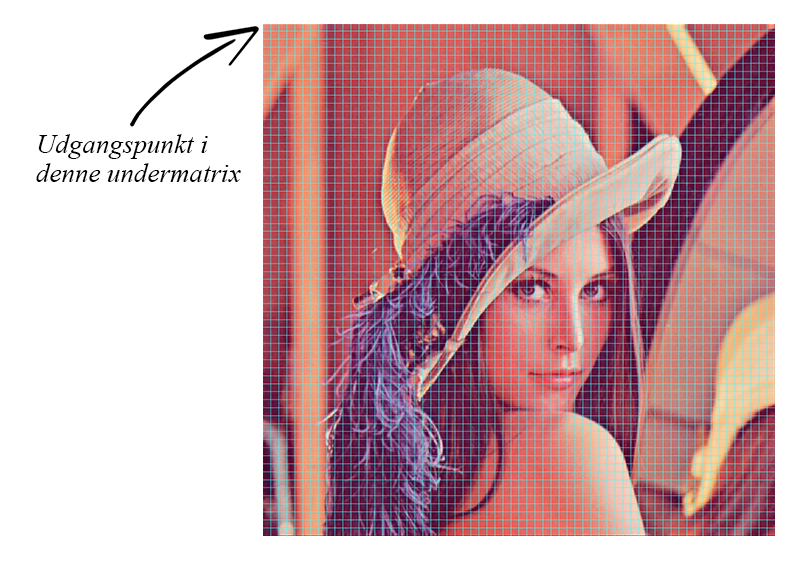
\includegraphics[width=0.5\textwidth]{billeder/lena-grid.png}
\caption{Lena delt op i 4096, $8 \times 8$ undermatricer.}
\label{fig:lena-grid-8x8}
\end{figure}
Herfra udføres DCT på undermatricen, og B findes vha. $B = U \boldsymbol{\cdot} A \boldsymbol{\cdot} U^T$, hvor $U$ og $U^T$ er givet i udtryk \vref{eq:DCTmatrix}.
\begin{figure}[!h]
\begin{minipage}[b]{0.25\linewidth}
\centering

\includegraphics[width=0.9\textwidth]{Billeder/LenaAnvendelse/RED8x8/lena2-R8x8-DCT.png}
\caption{DCT - Visuel.}
\label{fig:lena2-R8x8-DCT-visuel}
\end{minipage}
\hspace{0.5cm}
\begin{minipage}[b]{0.40\linewidth}
\centering
\[B_{1,\ 1}=\begin{bmatrix}
791    & -71  & 8,12   & 4,23   & -1,8  & -3,6  & -1,2  & 2,49   \\
-1,5  & 0,43  & 0,01   & 1,90   & 0,78  & 1,25   & -3,4  & -0,9 \\
-0,7 & -0,8 & -0,7 & -0,9 & -0,1 & -0,2 & 0,93  & 1,02   \\
2,66   & 1,02   & 1,38   & 0,21  & -0,5 & -0,5 & 0,95  & -1,3  \\
-3,3  & -0,9 & -1,5  & -0,2 & 0,75  & 0,18  & -1,0  & 1,55   \\
2,40   & 0,53  & 1,12   & 0,85  & -0,6 & 0,75  & -0,4 & -1,7  \\
-1,1  & -0,1 & -0,6 & -1,3  & 0,32  & -1,4  & 1,75   & 1,50   \\
0,21  & -0,1 & 0,18  & 0,98  & -0,1 & 1,15   & -1,6  & -0,9 \\
\end{bmatrix}\]
\caption{DCT - Tal.}
\label{fig:lena2-R8x8-DCT-matrix}
\end{minipage}
\end{figure}
Det ses tydeligt på den visuelle figur \ref{fig:lena2-R8x8-DCT-visuel}, hvordan alle overflødige høje frekvenser allerede er reduceret kraftigt. Dette er nøjagtigt det, som ønskes af DCT'en, da de lave frekvenser kan ses tydeligere af øjet end de høje. Den visuelle repræsentation er fremkommet ved at trunkere dataene til intervallet $[0;255]$. Næste trin i algoritmen er kvantiseringen, hvor der i dette eksempel tages udgangspunkt i $Q50$ jævnfør \vref{eq:Q50teori}. Den afrundede $C$ findes vha. \vref{C_beregning}
\begin{figure}[!h]
\begin{minipage}[b]{0.25\linewidth}
\centering

\includegraphics[width=0.9\textwidth]{Billeder/LenaAnvendelse/RED8x8/lena3-R8x8-quantization.png}
\caption{Kvantisering - Visuel.}
\label{fig:lena3-R8x8-quantization-visuel}
\end{minipage}
\hspace{0.5cm}
\begin{minipage}[b]{0.40\linewidth}
\centering
\[C_{1,\ 1}=\begin{bmatrix}
49 & -1 & 1 & . & . & . & . & . \\
.  & .  & . & . & . & . & . & . \\
.  & .  & . & . & . & . & . & . \\
.  & .  & . & . & . & . & . & . \\
.  & .  & . & . & . & . & . & . \\
.  & .  & . & . & . & . & . & . \\
.  & .  & . & . & . & . & . & . \\
.  & .  & . & . & . & . & . & . \\
\end{bmatrix}\]
\caption{Kvantisering - Tal.}
\label{fig:lena3-R8x8-quantization-matrix}
\end{minipage}
\end{figure}
Bemærk at der bruges indgangsvis division. Det ses, jævnfør tallene på figur \ref{fig:lena3-R8x8-quantization-matrix}, at matricen hovedsageligt udgøres af nuller. Dette er essentielt for Huffmankodningen, da den nu effektivt kan komprimere. Huffmantræet for undermatricen kan ses på figur \ref{fig:Huffman-8x8-visuel}. Tallene uden parentes repræsenterer hyppigheden af tallene i parentes.
\begin{figure}[htbp]
\centering
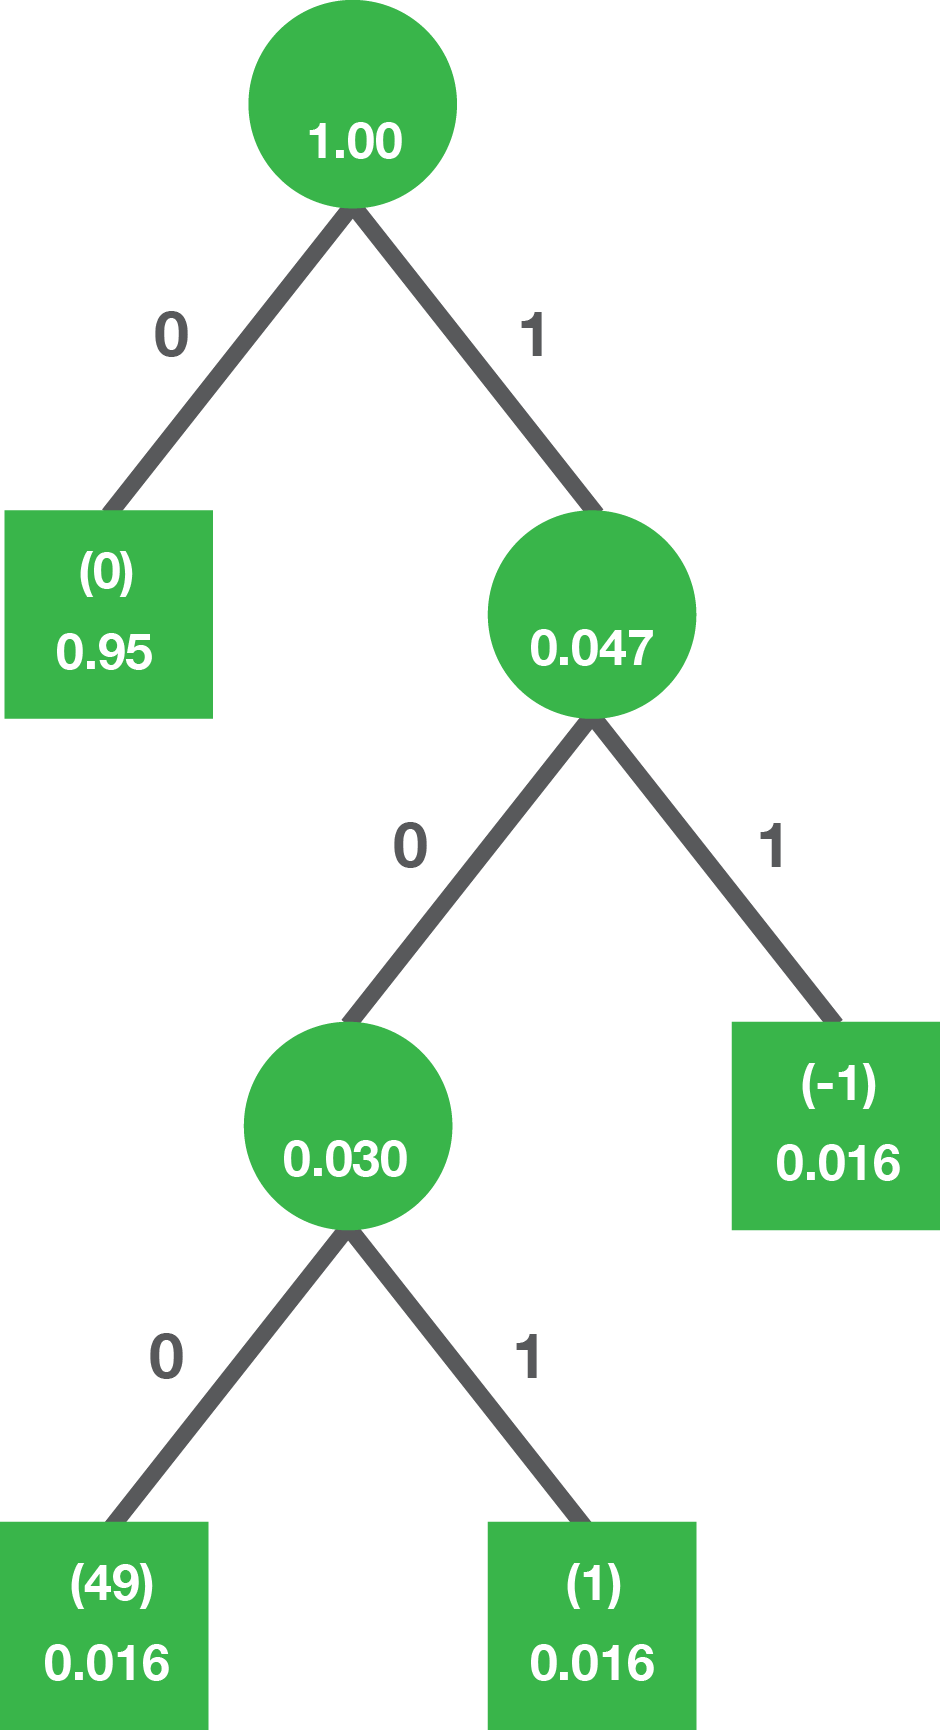
\includegraphics[width=0.25\textwidth]{Billeder/LenaAnvendelse/HUFFMAN/Huffman-8x8.png}
\caption{Huffmantræ for undermatricen.}
\label{fig:Huffman-8x8-visuel}
\end{figure}

Træet havde mildt sagt været markant større, hvis at Huffmantræet var lavet ud fra eksempelvis
 $A_{1,\ 1}$ eller $B_{1,\ 1}$. Her er det åbenlyst hvordan de to nævnte matricer, kun er \textit{forberedende} for en effektiv komprimering.

Der kan med fordel opstilles en tabel med relevante observationer fra Huffmantræet og dens resultater, se tabel \ref{tb:Huffman-8x8}. Den binære form blev fundet jævnfør \vref{sec:huffmanteori}.
\begin{table}[!h]
\centering
\begin{tabular}{|l|l|l|l|}
\hline
\textbf{Indgangsværdi} & \textbf{Antal} & \textbf{Sandsynlighed}      & \textbf{Binær form} \\ \hline
49                & 1              & $\frac{1}{64} \approx 0,016$ & 100                 \\ \hline
1                 & 1              & $\frac{1}{64} \approx 0,016$ & 101                 \\ \hline
-1                & 1              & $\frac{1}{64} \approx 0,016$ & 11                  \\ \hline
0                 & 61             & $\frac{61}{64} \approx 0,95$ & 0                   \\ \hline
\end{tabular}
\caption{Huffmantræet i tabelform}
\label{tb:Huffman-8x8}
\end{table}
I binær form vil undermatricen nu hedde: $$ 100110001010000000000000000000000000000000000000000000000000000000000 $$
En komprimeret fil er opnået, og den lange streng af nuller resulterer i, at filen fylder mindre, end hvis Huffmankodningen var blevet gjort før kvantiseringen. Jævnfør algoritmen på side \pageref{tb:Algoritme-Dekomprimering-DCT} udføres \textit{de}komprimeringen, hvilket gøres med de modsatte regneoperationer i forhold til komprimeringen.
\begin{table}[!h]
\centering
\begin{tabular}{lll}
\hline
\multicolumn{2}{l}{\textbf{Algoritme: Dekomprimering vha. DCT}}    &                                                                   \\ \hline
\\
\multicolumn{1}{|l}{1.}        & Input:                     & Komprimeret fil \\
\multicolumn{1}{|l}{2.}        & Output:                    & Dekomprimeret billede, $A'$                                           \\
                               &                            &                                                                   \\
\multicolumn{2}{|l}{\textit{Dekomprimering (invers proces)}} &                                                                   \\
\multicolumn{1}{|l}{9.}        & Entropidekodning:         & Filen dekomprimeres vha. Huffman til $C'$             \\
\multicolumn{1}{|l}{10.}        & Dekvantisering:            & $B' = Q_{(i,\ j)} \cdot C'_{(i,\ j)}$                                                 \\
\multicolumn{1}{|l}{11.}       & Invers DCT / DCT-III:      & $A' = U^T \boldsymbol{\cdot} B' \boldsymbol{\cdot} U$\\
\multicolumn{1}{|l}{12.}       & Decentrering omkring 0:      & $A' = A' + 128$ indgangsvist\\
\multicolumn{1}{|l}{13.}       & Samling:                   & $8 \times 8$ matricer samles til ét billede
\\  
\end{tabular}
\label{tb:Algoritme-Dekomprimering-DCT}
\end{table}
Resultatet af den inverse algoritme på $A_{(1,\ 1)}$ resulterer i værdierne illustreret i figur \ref{fig:lena4-R8x8-compressed-visuel} og \ref{fig:lena4-R8x8-decompressed-matrix}.
\begin{figure}[htbp]
\begin{minipage}[b]{0.27\linewidth}
\centering
\includegraphics[width=0.8\textwidth]{Billeder/LenaAnvendelse/RED8x8/lena4-R8x8-compressed.png}
\caption{Dekomprimeret - Visuel.}
\label{fig:lena4-R8x8-compressed-visuel}
\end{minipage}
\hspace{0.5cm}
\begin{minipage}[b]{0.45\linewidth}
\centering
\[\resizebox{0.9\textwidth}{!}{$C_{1,\ 1}=\begin{bmatrix}
226 & 225 & 224 & 224 & 225 & 226 & 228 & 230 \\
226 & 225 & 224 & 224 & 225 & 226 & 228 & 230 \\
226 & 225 & 224 & 224 & 225 & 226 & 228 & 230 \\
226 & 225 & 224 & 224 & 225 & 226 & 228 & 230 \\
226 & 225 & 224 & 224 & 225 & 226 & 228 & 230 \\
226 & 225 & 224 & 224 & 225 & 226 & 228 & 230 \\
226 & 225 & 224 & 224 & 225 & 226 & 228 & 230 \\
226 & 225 & 224 & 224 & 225 & 226 & 228 & 230 \\
\end{bmatrix}$}\]
\caption{Dekomprimeret - Tal.}
\label{fig:lena4-R8x8-decompressed-matrix}
\end{minipage}
\end{figure}
Den umiddelbare største ændring af undermatricen er dens endnu mere ensartethed. Da der ikke forekommer drastiske spring i overgangene mellem pixelene ser den monoton ud. Det er svært for det menneskelige øje, at skældne mellem denne undermatrice og den oprindelige, hvilket var intentionen i første omgang. 
For referencens skyld udføres algoritmen på hele Lena i de følgende figurer. Det undlades dog at vise den binære form.
%\begin{figure}[!h]
%\begin{minipage}{0.45\textwidth}
%\centering
%\includegraphics[width=0.4\textwidth]{Billeder/LenaAnvendelse/LENABILLEDE/lena2-DCT.png}
%\caption{DCT - Lena.}
%\label{fig:lena2-DCT-visuel}
%\end{minipage}
%\hspace{0.5cm}
%\begin{minipage}{0.45\textwidth}
%\centering
%\includegraphics[width=0.4\textwidth]{Billeder/LenaAnvendelse/LENABILLEDE/lena4-enhanced-quantization2.png}
%\caption{Kvantisering - Lena.}
%\label{fig:lena4-enhanced-quantization-visuel}
%\end{minipage}
%\end{figure}
\begin{figure}[htbp]
\begin{minipage}{0.3\textwidth}
\centering
\includegraphics[width=0.9\textwidth]{Billeder/LenaAnvendelse/LENABILLEDE/lena5-compressed.png}
\caption{\href{https://www.dropbox.com/home/P1\%20-\%20B205/vejleder/billeder/DCT/Lena\%20ved\%20forskelige\%20Q?preview=lenaQ50.png}{Dekomprimeret - Lena.}}
\label{fig:lena5-decompressed-visuel}
\end{minipage}
\hspace{0.5cm}
\begin{minipage}{0.3\textwidth}
\centering
\includegraphics[width=0.9\textwidth]{Billeder/fejlbilleder/fejl50.png}
\caption{\href{https://www.dropbox.com/home/P1\%20-\%20B205/vejleder/billeder/DCT/Fejlbilleder?preview=fejl50.png}{Fejlbillede - Lena.}}
\label{fig:lena1-org-fejl}
\end{minipage}
\hspace{0.5cm}
\begin{minipage}{0.3\textwidth}
\centering
\includegraphics[width=0.9\textwidth]{Billeder/LenaAnvendelse/LENABILLEDE/lena1-org.png}
\caption{\href{https://www.dropbox.com/home/P1\%20-\%20B205/vejleder/billeder?preview=lena-org.tiff}{Oprindelig - Lena.}}
\label{fig:lena1-org-visuel}
\end{minipage}
\end{figure}
Jævnfør \ref{fig:lena5-decompressed-visuel} og \ref{fig:lena1-org-visuel} er det svært at skelne mellem billederne. Dette forstærkes ydermere af fejlbilledet, der illustrerer forskellen mellem det nye og det oprindelige billede. Grå illustrerer ingen forskel, sort illustrerer en mørkere farve i det nye billede, og ligeså illustrerer en lysere farve, at det nye billede er blevet lysere. En farvenuance illustrerer en farveforskel. Hensigten er opnået; billedet har ikke ændret sig betydeligt, og filstørrelsen er komprimeret i forhold til før algoritmen.
%\section{DCT anvendelse} \label{sec:DCTAnvendelse}
I dette afsnit undersøges den praktiske anvendelse af DCT, jævnfør kapitel \ref{chapter:DCT}, hvilket udføres på billedet af Lena, se figur \vref{fig:lena-grid-8x8}. Billedet har dimensionerne $ 512 \times \SI{512}{pixel}$, hvilket indledningsvist opdeles i $8 \times 8$ undermatricer. Endvidere er der $ 64 \cdot 64$ matricer af $8 \times 8$, hvilket giver $64 \cdot 64 \cdot 8 \cdot 8 = 262.144$ pixels totalt.

De følgende regneoperationer bliver kun udført på den røde farvekanal og første $8 \times 8$ undermatrix for at vise princippet ved brugen af metoden. Ved gentagelse med resten af undermatricerne og de resterende to farvekanaler opnås en komprimering af det fulde farvebillede. Repetitionerne af beregningerne udelades, da dette blot er et eksempel. Derimod \textit{vises} resultatet af komprimeringen for hele billedet, efter regneeksemplet med undermatricen er udført. For at skabe overblik over komprimeringen ses komprimeringsalgoritmen herunder:
\begin{table}[!h]
\centering
\begin{tabular}{lll}
\hline
\multicolumn{3}{l}{\textbf{Algoritme: Komprimering vha. DCT}}                           \\ \hline
\\
\multicolumn{1}{|l}{1.}        & Input:                     & Billede, $A$: $m \times n$ pixels             \\
\multicolumn{1}{|l}{2.}        & Output:                    & Komprimeret fil       \\
                               &                            &                        \\
\multicolumn{2}{|l}{\textit{Komprimering}}                  &                        \\
\multicolumn{1}{|l}{3.}        & Opdeling:                  & Billede opdeles i farvekanaler og $8 \times 8$ matricer \\
\multicolumn{1}{|l}{4.}        & Centrering omkring 0:      & $A = A - 128$ indgangsvist    \\
\multicolumn{1}{|l}{5.}        & DCT:              & $B = U \boldsymbol{\cdot} A \boldsymbol{\cdot} U^T$  \\
\multicolumn{1}{|l}{6.}        & Kvantisering:              & $\lfloor C_{(i,\ j)} \rceil = \frac{B_{(i,\ j)}}{Q_{(i,\ j)}}$ afrundet\\
\multicolumn{1}{|l}{7.}        & Entropi kodning:           & $C$ komprimeres vha. Huffman til en fil              \\
\multicolumn{1}{|l}{8.}        & Gentagelse:                & Ovenstående gentages for samtlige $8 \times 8$ matricer\\
\end{tabular}
\label{tb:Algoritme-Komprimering-DCT}
\end{table}

Den specifikke undermatrix i følgende eksempel ligger i øverste venstre hjørne, jævnfør figur \vref{fig:lena-grid-8x8}. Første værdi for hver indgang, dvs. den røde kanal, findes vha. vores Python-program og følgende undermatrix, $A_{1,1}$, fremkommer.

\begin{figure}[!h]
\begin{minipage}[b]{0.27\linewidth}
\centering
\includegraphics[width=\textwidth]{Billeder/LenaAnvendelse/RED8x8/lena1-R8x8-org.png}
\caption{Oprindelig - Visuel.}
\label{fig:lena1-R8x8-org-visuel}
\end{minipage}
\hspace{0.5cm}
\begin{minipage}[b]{0.45\linewidth}
\centering
\[A_{1,1}=\begin{bmatrix}
226 & 226 & 223 & 223 & 226 & 226 & 228 & 227 \\
226 & 226 & 223 & 223 & 226 & 226 & 228 & 227 \\
226 & 226 & 223 & 223 & 226 & 226 & 228 & 227 \\
226 & 226 & 223 & 223 & 226 & 226 & 228 & 227 \\
226 & 226 & 223 & 223 & 226 & 226 & 228 & 227 \\
227 & 227 & 227 & 222 & 226 & 228 & 226 & 230 \\
228 & 228 & 225 & 224 & 225 & 229 & 229 & 229 \\
223 & 223 & 226 & 221 & 227 & 225 & 226 & 228 \\
\end{bmatrix}\]
\caption{Oprindelig - Tal.}
\label{fig:lena1-R8x8-org-matrix}
\end{minipage}
\end{figure}

\begin{figure}[htbp]
\centering
\includegraphics[width=0.7\textwidth]{billeder/lena-grid.png}
\caption{Lena delt op i 4096, $8 \times 8$ undermatricer.}
\label{fig:lena-grid-8x8}
\end{figure}

Herfra udføres DCT på undermatricen, og B findes vha. $B = U \boldsymbol{\cdot} A \boldsymbol{\cdot} U^T$, hvor $U$ og $U^T$ er givet i udtryk \vref{eq:DCTmatrix}.

\begin{figure}[!h]
\begin{minipage}[b]{0.25\linewidth}
\centering
\includegraphics[width=\textwidth]{Billeder/LenaAnvendelse/RED8x8/lena2-R8x8-DCT.png}
\caption{DCT - Visuel.}
\label{fig:lena2-R8x8-DCT-visuel}
\end{minipage}
\hspace{0.5cm}
\begin{minipage}[b]{0.40\linewidth}
\centering
\[B_{1,\ 1}=\begin{bmatrix}
791    & -71  & 8,12   & 4,23   & -1,8  & -3,6  & -1,2  & 2,49   \\
-1,5  & 0,43  & 0,01   & 1,90   & 0,78  & 1,25   & -3,4  & -0,9 \\
-0,7 & -0,8 & -0,7 & -0,9 & -0,1 & -0,2 & 0,93  & 1,02   \\
2,66   & 1,02   & 1,38   & 0,21  & -0,5 & -0,5 & 0,95  & -1,3  \\
-3,3  & -0,9 & -1,5  & -0,2 & 0,75  & 0,18  & -1,0  & 1,55   \\
2,40   & 0,53  & 1,12   & 0,85  & -0,6 & 0,75  & -0,4 & -1,7  \\
-1,1  & -0,1 & -0,6 & -1,3  & 0,32  & -1,4  & 1,75   & 1,50   \\
0,21  & -0,1 & 0,18  & 0,98  & -0,1 & 1,15   & -1,6  & -0,9 \\
\end{bmatrix}\]
\caption{DCT - Tal.}
\label{fig:lena2-R8x8-DCT-matrix}
\end{minipage}
\end{figure}

Det ses tydeligt på den visuelle figur \ref{fig:lena2-R8x8-DCT-visuel}, hvordan alle overflødige høje frekvenser allerede er reduceret kraftigt. Dette er nøjagtigt det, som ønskes af DCT'en, da de lave frekvenser kan ses tydeligere af øjet end de høje. Den visuelle repræsentation er fremkommet ved at trunkere dataene til intervallet $[0;255]$. Næste trin i algoritmen er kvantiseringen, hvor der i dette eksempel tages udgangspunkt i $Q50$ jævnfør \vref{eq:Q50teori}. Den afrundede $C$ findes vha. $\lfloor C_{(i,\ j)} \rceil = \frac{B_{(i,\ j)}}{Q50_{(i,\ j)}}$:

\begin{figure}[!h]
\begin{minipage}[b]{0.25\linewidth}
\centering
\includegraphics[width=\textwidth]{Billeder/LenaAnvendelse/RED8x8/lena3-R8x8-quantization.png}
\caption{Kvantisering - Visuel.}
\label{fig:lena3-R8x8-quantization-visuel}
\end{minipage}
\hspace{0.5cm}
\begin{minipage}[b]{0.40\linewidth}
\centering
\[C_{1,\ 1}=\begin{bmatrix}
49 & -1 & 1 & . & . & . & . & . \\
.  & .  & . & . & . & . & . & . \\
.  & .  & . & . & . & . & . & . \\
.  & .  & . & . & . & . & . & . \\
.  & .  & . & . & . & . & . & . \\
.  & .  & . & . & . & . & . & . \\
.  & .  & . & . & . & . & . & . \\
.  & .  & . & . & . & . & . & . \\
\end{bmatrix}\]
\caption{Kvantisering - Tal.}
\label{fig:lena3-R8x8-quantization-matrix}
\end{minipage}
\end{figure}

Bemærk at der bruges indgangsvis division. Det ses, jævnfør tallene på figur \ref{fig:lena3-R8x8-quantization-matrix}, at matricen hovedsageligt udgøres af nuller. Dette er essentielt for Huffmankodningen, da den nu effektivt kan komprimere. Huffman-træet for undermatricen kan ses på figur \ref{fig:Huffman-8x8-visuel}. Tallene uden parentes repræsenterer hyppigheden af tallene i parentes.
\begin{figure}[htbp]
\centering
\includegraphics[width=0.25\textwidth]{Billeder/LenaAnvendelse/HUFFMAN/Huffman-8x8.png}
\caption{Huffman-træ for undermatricen.}
\label{fig:Huffman-8x8-visuel}
\end{figure}

Træet havde mildt sagt været markant større, hvis at Huffmantræet var lavet ud fra eksempelvis  $A_{1,\ 1}$ eller $B_{1,\ 1}$. Her er det åbenlyst hvordan de to nævnte matricer, kun er \textit{forberedende} for en effektiv komprimering.

Der kan med fordel opstille en tabel med relevante observationer fra Huffmantræet og dens resultater, se tabel \ref{tb:Huffman-8x8}. Den binære form blev fundet jævnfør \vref{sec:huffmanteori}.

\begin{table}[!h]
\centering
\begin{tabular}{|l|l|l|l|}
\hline
\textbf{Indgangsværdi} & \textbf{Antal} & \textbf{Sandsynlighed}      & \textbf{Binær form} \\ \hline
49                & 1              & $\frac{1}{64} \approx 0,016$ & 100                 \\ \hline
1                 & 1              & $\frac{1}{64} \approx 0,016$ & 101                 \\ \hline
-1                & 1              & $\frac{1}{64} \approx 0,016$ & 11                  \\ \hline
0                 & 61             & $\frac{61}{64} \approx 0,95$ & 0                   \\ \hline
\end{tabular}
\caption{Huffman-træet i tabelform}
\label{tb:Huffman-8x8}
\end{table}

I binær form vil undermatricen nu hedde: $$ 100110001010000000000000000000000000000000000000000000000000000000000 $$
En komprimeret fil er opnået, og den lange streng af nuller resulterer i, at filen fylder mindre, end hvis Huffmankodningen var blevet gjort før kvantiseringen. Jævnfør algoritmen på side \pageref{tb:Algoritme-Dekomprimering-DCT} udføres \textit{de}komprimeringen, hvilket gøres med de modsatte regneoperationer i forhold til komprimeringen.

\begin{table}[!h]
\centering
\begin{tabular}{lll}
\hline
\multicolumn{2}{l}{\textbf{Algoritme: Dekomprimering vha. DCT}}    &                                                                   \\ \hline
\\
\multicolumn{1}{|l}{1.}        & Input:                     & Komprimeret fil \\
\multicolumn{1}{|l}{2.}        & Output:                    & Dekomprimeret billede, $A'$                                           \\
                               &                            &                                                                   \\
\multicolumn{2}{|l}{\textit{Dekomprimering (invers proces)}} &                                                                   \\
\multicolumn{1}{|l}{9.}        & Entropi dekodning:         & Filen dekomprimeres vha. Huffman til $C'$             \\
\multicolumn{1}{|l}{10.}        & Dekvantisering:            & $B' = Q_{(i,\ j)} \cdot C'_{(i,\ j)}$                                                 \\
\multicolumn{1}{|l}{11.}       & Invers DCT / DCT-III:      & $A' = U^T \boldsymbol{\cdot} B' \boldsymbol{\cdot} U$\\
\multicolumn{1}{|l}{12.}       & Decentrering omkring 0:      & $A' = A' + 128$ indgangsvist\\
\multicolumn{1}{|l}{13.}       & Samling:                   & $8 \times 8$ matricer samles til ét billede
\\  
\end{tabular}
\label{tb:Algoritme-Dekomprimering-DCT}
\end{table}

Resultatet af den inverse algoritme på $A_{(1,\ 1)}$ ender med følgende værdierne som illustreret i figur \ref{fig:lena4-R8x8-compressed-visuel} og \ref{fig:lena4-R8x8-decompressed-matrix}.

\begin{figure}[htbp]
\begin{minipage}[b]{0.27\linewidth}
\centering
\includegraphics[width=\textwidth]{Billeder/LenaAnvendelse/RED8x8/lena4-R8x8-compressed.png}
\caption{Dekomprimeret - Visuel.}
\label{fig:lena4-R8x8-compressed-visuel}
\end{minipage}
\hspace{0.5cm}
\begin{minipage}[b]{0.45\linewidth}
\centering
\[C_{1,\ 1}=\begin{bmatrix}
226 & 225 & 224 & 224 & 225 & 226 & 228 & 230 \\
226 & 225 & 224 & 224 & 225 & 226 & 228 & 230 \\
226 & 225 & 224 & 224 & 225 & 226 & 228 & 230 \\
226 & 225 & 224 & 224 & 225 & 226 & 228 & 230 \\
226 & 225 & 224 & 224 & 225 & 226 & 228 & 230 \\
226 & 225 & 224 & 224 & 225 & 226 & 228 & 230 \\
226 & 225 & 224 & 224 & 225 & 226 & 228 & 230 \\
226 & 225 & 224 & 224 & 225 & 226 & 228 & 230 \\
\end{bmatrix}\]
\caption{Dekomprimeret - Tal.}
\label{fig:lena4-R8x8-decompressed-matrix}
\end{minipage}
\end{figure}

Den umiddelbare største ændring af undermatricen er dens endnu mere ensartethed. Da der ikke forekommer drastiske spring i overgangene mellem pixelene ser den monoton ud. Det er svært for det menneskelige øje, at skældne mellem denne undermatrice og den oprindelige, hvilket var intentionen i første omgang. 
For referencens skyld udføres algoritmen på hele Lena-billedet i de følgende figurer. Det undlades dog at vise den binære form.

%\begin{figure}[!h]
%\begin{minipage}{0.45\textwidth}
%\centering
%\includegraphics[width=0.4\textwidth]{Billeder/LenaAnvendelse/LENABILLEDE/lena2-DCT.png}
%\caption{DCT - Lena.}
%\label{fig:lena2-DCT-visuel}
%\end{minipage}
%\hspace{0.5cm}
%\begin{minipage}{0.45\textwidth}
%\centering
%\includegraphics[width=0.4\textwidth]{Billeder/LenaAnvendelse/LENABILLEDE/lena4-enhanced-quantization2.png}
%\caption{Kvantisering - Lena.}
%\label{fig:lena4-enhanced-quantization-visuel}
%\end{minipage}
%\end{figure}
\begin{figure}[htbp]
\begin{minipage}{0.3\textwidth}
\centering
\includegraphics[width=0.9\textwidth]{Billeder/LenaAnvendelse/LENABILLEDE/lena5-compressed.png}
\caption{\href{https://www.dropbox.com/home/P1\%20-\%20B205/vejleder/billeder/DCT/Lena\%20ved\%20forskelige\%20Q?preview=lenaQ50.png}{Dekomprimeret - Lena.}}
\label{fig:lena5-decompressed-visuel}
\end{minipage}
\hspace{0.5cm}
\begin{minipage}{0.3\textwidth}
\centering
\includegraphics[width=0.9\textwidth]{Billeder/fejlbilleder/fejl50.png}
\caption{\href{https://www.dropbox.com/home/P1\%20-\%20B205/vejleder/billeder/DCT/Fejlbilleder?preview=fejl50.png}{Fejlbillede - Lena.}}
\label{fig:lena1-org-fejl}
\end{minipage}
\hspace{0.5cm}
\begin{minipage}{0.3\textwidth}
\centering
\includegraphics[width=0.9\textwidth]{Billeder/LenaAnvendelse/LENABILLEDE/lena1-org.png}
\caption{\href{https://www.dropbox.com/home/P1\%20-\%20B205/vejleder/billeder?preview=lena-org.tiff}{Oprindelig - Lena.}}
\label{fig:lena1-org-visuel}
\end{minipage}
\end{figure}

Jævnfør \ref{fig:lena5-decompressed-visuel} og \ref{fig:lena1-org-visuel} er det enormt svært at skelne mellem billederne. Dette forstærkes ydermere af fejlbilledet, der illustrerer forskellen mellem det nye og det oprindelige billede. Grå illustrerer ingen forskel, sort illustrerer en mørkere farve i det nye billede, og ligeså illustrerer en lysere farve, at det nye billede er blevet lysere. En farvenuance illustrerer en farveforskel. Hensigten er opnået; billedet har ikke ændret sig betydeligt, og filstørrelsen er komprimeret i forhold til før algoritmen.

%% Afrunding %%

\chapter{Resultater}\label{chapter:resultater}
I det følgende afsnit, bliver resultaterne fra komprimering af Lena med hhv. DCT og PCA præsenteret. Resultaterne vil i afsnit \ref{sec:vurdering} blive brugt til at sammenligne de to komprimeringsmetoder.

I forhold til den opstillede case er det interressant at kigge på forskellige parametre: komprimeringsgrad og billedekvalitet. Disse parametre er interessante, da det ønskes at nedbringe filstørrelsen, så en mobilbruger har plads til flere billeder på telefonen af gangen. Ydermere ønskes det, at brugeroplevelsen ikke skal påvirkes af komprimeringen, hvilket imidlertid betyder, at billedekvaliteten skal bibeholdes mest muligt.

Der er med hhv. DCT og PCA lavet test med forskellige grader af komprimering, hvor alle parametre er blevet målt med henblik på sammenligning af DCT og PCA som komprimeringsmetoder. Komprimeringer med DCT er lavet med følgende $Q$-værdier: $10$, $25$, $50$, $75$ og $90$. PCA-komprimeringerne er målt med følgende antal principale komponenter: $1$, $5$, $10$, $15$, $20$, $25$, $50$, $75$, $100$, $150$, $200$ og $512$. \\
Der tages først udgangspunkt i komprimeringsgraden for de forskellige komprimeringer.

\section{Komprimeringsgrad}
Først ses der nærmere på DCTs og PCAs evne til at komprimere den originale fil til en mindre fil. Filstørrelsen for DCT måles i bitrepræsentationen fra en TXT-fil, der er Huffmankodet. Det er dermed ikke TXT-filens faktiske størrelse, da fokusset i dette projekt har været på matematikken bag komprimeringen og ikke datastrukturen i en binær fil. Ligeledes måles filstørrelsen af de PCA-komprimerede filer ved den totale længde af bitrepræsentationen i filen. \\
Den oprindelige filstørrelse betragtes som værende det totale antal pixels i alle farverum multipliceret med otte, da hvert tal repræsenteres med otte bit. Dette giver en filstørrelse på $512\cdot512\cdot3\cdot8 = 6.291.456$ bit for det oprindelige billede. Komprimeringsgraden er beregnet som $$\text{Komprimeringsgrad} = \frac{\text{Oprindelig filstørrelse}}{\text{Komprimeret filstørrelse}}$$
Tabel \ref{tb:komprimering_DCT}, \ref{tb:komprimering_PCA1} og \vref{tb:komprimering_PCA2} præsenterer komprimeringsgraden for de forskellige komprimeringer med de to metoder.
\begin{table}[htbp]
\centering
\begin{tabular}{|l|l|l|l|l|l|l|}	\hline
\textbf{DCT}					& \textbf{Q10}		& \textbf{Q25}		& \textbf{Q50}			& \textbf{Q75}			& \textbf{Q90}		\\ \hline
\textbf{Bit}					& 860.718	& 943.432	& 1.051.307		& 1.228.152		& 1.658.414	\\ \hline
\textbf{Kompressionsgrad}	& 1:7,31		& 1:6,67		& 1:5,98			& 1:5,12			& 1:3,79		\\ \hline
\end{tabular}
\caption{Komprimeringsgrad med DCT ved forskellige $Q$}
\label{tb:komprimering_DCT}
\end{table}
\begin{table}[htbp]
\centering
\begin{tabular}{|l|l|l|l|l|l|l|l|l|l|l|l|l|}	\hline
\textbf{PCA} 				& \textbf{PC1}  		& \textbf{PC5}		& \textbf{PC10}		& \textbf{PC15}		& \textbf{PC20}		& \textbf{PC25}		\\ \hline
\textbf{Bit}  			& 64.385 	& 207.719	& 371.527	& 532.286	& 532.286	& 845.598	\\ \hline
\textbf{Kompressionsgrad}	& 1:97,72	& 1:30,29	& 1:16,93	& 1:11,82	& 1:9,12 	& 1:7,44	\\ \hline
\end{tabular}
\caption{Komprimeringsgrad med PCA ved forskellige antal PC}
\label{tb:komprimering_PCA1}
\end{table}
\begin{table}[htbp]
\centering
\begin{tabular}{|l|l|l|l|l|l|l|l|l|l|l|l|l|}	\hline
\textbf{PCA}					& \textbf{PC50}  		& \textbf{PC75}   		& \textbf{PC100}  		& \textbf{PC150}	& \textbf{PC200}			& \textbf{PC512}   		\\ \hline
\textbf{Bit	}				& 1.606.858		& 2.346.277		& 3.066.789
&4.475.223 	& 5.836.314		& 13.473.311 	\\ \hline
\textbf{Kompressionsgrad}		& 1:3,92			& 1:3,39			& 1:2,05	 & 1:1,41		& 1:1,08		& 1:0,47		\\ \hline
\end{tabular}
\caption{Komprimeringsgrad med PCA ved forskellige antal PC}
\label{tb:komprimering_PCA2}
\end{table}

Bemærk her er komprimeringsgraden under 1 ved 512 PC'er (fremover forkortes førnævnte som PC512). Dette skyldes at filstørrelsen tilnærmelsesvist (der ses her bort fra Huffmankodning, og at der kan kræves mere end otte bit pr. tal), kan findes ved $\Big(\big((PC \cdot 512) + (PC \cdot 512) + (1 \cdot 512)\big) \cdot 3 \Big) \cdot 8$, hvor det er tydeligt at ved PC256 gemmes flere data end i det oprindelige billede, hvorved at komprimeringen er ikke-eksisterende - altså forøges filstørrelsen, hvilket selvsagt ikke er ønskværdigt.

\section{Kvalitet}
Billedekvaliteten af de komprimerede billeder skal vurderes for at sikre, at billederne ikke blot komprimeres, men at de også stadig repræsenterer det samme billede uden for mange forvrængninger. Dette kan gøres både som en subjektiv undersøgelse med en repræsentativ gruppe af mobilbrugere, og der kan objektivt undersøges parametre for kvaliteten af billedet i form af, hvor meget pixelværdierne har ændret sig, hvor mange pixels, der er ændret såvel som den maksimale og minimale ændring af disse pixelændringer. De sidstnævnte parametre giver et objektivt indblik i, hvordan billedet har ændret sig.

\begin{table}[htbp]
\begin{minipage}[b]{0.45\linewidth}\centering
\begin{tabular}{|l|c|}
\hline
    & \textbf{Ændrede pixels} \\ \hline
\textbf{Q10} & 96,16     \%           \\ \hline
\textbf{Q25} & 94,03     \%           \\ \hline
\textbf{Q50} & 92,78     \%           \\ \hline
\textbf{Q75} & 91,67     \%           \\ \hline
\textbf{Q90} & 89,38     \%           \\ \hline
\end{tabular}
\caption{Procentvise pixelændring, med DCT, i det dekomprimerede billede i forhold til det originale}
\label{tb:procent_DCT}
\end{minipage}
\hspace{0.5cm}
\begin{minipage}[b]{0.45\linewidth}
\centering
\begin{tabular}{|l|c|}
\hline
      & \textbf{Ændrede pixels} \\ \hline
\textbf{PC1}   & 98,93   \%     \\ \hline
\textbf{PC5}   & 98,08   \%     \\ \hline
\textbf{PC10}  & 97,11   \%     \\ \hline
\textbf{PC15}  & 96,61   \%     \\ \hline
\textbf{PC20}  & 96,12   \%     \\ \hline
\textbf{PC25}  & 95,53   \%     \\ \hline
\textbf{PC50}  & 94,02   \%     \\ \hline
\textbf{PC75}  & 92,65   \%     \\ \hline
\textbf{PC100} & 91,66   \%     \\ \hline
\textbf{PC150} & 88,83   \%     \\ \hline
\textbf{PC200} & 86,13   \%     \\ \hline
\textbf{PC512} & 80,36   \%     \\ \hline
\end{tabular}
\caption{Procentvise pixelændring, med PCA, i det dekomprimerede billede i forhold til det originale}
\label{tb:procent_PCA}
\end{minipage}
\end{table}

I tabel \ref{tb:procent_DCT} og \ref{tb:procent_PCA} er der udtrykt, hvor mange af de oprindelige pixels, der er blevet ændret i en eller anden grad i det dekomprimerede billde. Tabellerne udtrykker ikke direkte noget om graden af komprimering, eller hvor meget de enkelte pixels har ændret sig, men blot hvor mange pixels, der er blevet ændret. En procentvis ændring på ca. 90 \% kan derfor være misvisende, da dette virker som en stor ændring. Parametret siger altså ikke noget om, hvor stor graden af ændring er, og det må forventes, at store dele af disse ændringer er af ubetydelig størrelse. Alternativt kunne man bestemme en tolerance, så eksempelvis kun ændringer over fem bliver noteret. Med denne modificering ville parametret kunne sige mere om ændringernes effekt.

I de pixels, hvor der er sket en ændring af intensiteten, er det interessant at kigge på ift. hvor stor en grad, de er blevet ændret. Dette har betydning for brugerens oplevelse af, hvor meget billedet er ændret efter komprimeringen. En stor ændring i pixels udtrykker stor ændring i billedet og større chance for at bemærke ændringerne end ved små pixelændringer. Typisk fremkommer lignende afvigelser i samme områder, da begge metoder forsøger at skabe glatte overgange mellem de enkelte pixels.\\
Ændring i pixelværdier er i alle komprimeringer målt i alle tre farverum. Den gennemsnitlige ændring over alle farverum er tilmed beregnet. Bemærk at det er den absolutte pixelændring, der fremgår af figur \ref{fig:pixelchange_DCT_diagram} og \vref{fig:pixelchange_PCA_diagram}, hvorved der ikke differentieres mellem ændringer i positiv eller negativ retning. Ydermere er gennemsnittene beregnet ud fra antallet af pixels med ændringer, hvorved pixels uden ændring ikke medtages i disse beregninger.
For overblikkets skyld repræsenteres den gennemsnitlige ændring i pixelværdi i figur \ref{fig:pixelchange_DCT_diagram} og \ref{fig:pixelchange_PCA_diagram}.
%\begin{table}[htpb]
%\centering
%\begin{tabular}{|l|l|l|l|l|l|}
%\hline
%     	& Q10	& Q25	& Q50	& Q75	& Q90	\\ \hline
%Rød 		& 7.95	& 4.85	& 3.71	& 3.03	& 2.39	\\ \hline
%Grøn 	& 8.79	& 5.79	& 4.62	& 3.82	& 2.99	\\ \hline
%Blå  	& 8.73	& 6.19	& 5.21	& 4.47	& 3.51	\\ \hline
%Samlet 	& 8.49	& 5.61	& 4.51	& 3.77	& 2.96	\\ \hline
%	
%\end{tabular}
%\caption{Den største afvigelse for hver farve i DCT}
%\label{fig:pixelchange_DCT_tabel}
%\end{table}
%
%\begin{table}[htpb]
%\centering
%\begin{tabular}{|l|l|l|l|l|l|l|l|l|}
%\hline
%     & PCA1  & PCA5 	 & PCA10	  & PCA15  & PCA20	& PCA25\\\hline
%Rød  & 29.27 & 18.05  & 12.65  & 10.64  & 9.02	& 9.75	\\ \hline
%Grøn & 34.02 & 20.75  & 15.25  & 12.79  & 11.10	& 9.84	\\ \hline
%Blå  & 22.98 & 15.03  & 11.44  & 9.92   & 8.89	& 8.19	\\ \hline
%Samlet & 28.75 & 17.95 & 13.12 & 11.12  & 9.67	& 8.66	\\ \hline
%\end{tabular}
%\caption{Den største afvigelse for hver farve i PCA}
%\label{fig:pixelchange_PCA_tabel1}
%\end{table}
%\begin{table}[htpb]
%\centering
%\begin{tabular}{|l|l|l|l|l|l|l|l|l|}
%\hline
%		& PCA50	& PCA75	& PCA100		 & PCA150	& PCA200		& PCA512		\\ \hline
%Rød		& 5.25	& 3.89	& 3.10		 & 2.10		& 1.85 		& 1.26 		\\ \hline
%Grøn		& 6.85	& 5.28	& 4.24		 & 2.90		& 2.35 		& 1.27		\\ \hline
%Blå		& 6.26	& 5.22	& 4.48 		 & 3.37 		& 2.75 		& 1.28		\\ \hline
%Samlet	& 6.12	& 4.79	& 3.93 		 & 2.79 		& 2.32 		& 1.27		\\ \hline
%\end{tabular}
%\caption{Den største afvigelse for hver farve i PCA}
%\label{fig:pixelchange_PCA_tabel2}
%\end{table}

\definecolor{bblue}{HTML}{4F81BD}
\definecolor{rred}{HTML}{C0504D}
\definecolor{ggreen}{HTML}{9BBB59}
\definecolor{ggray}{HTML}{AAAAAA}
\begin{figure}[htbp]
\centering
\begin{tikzpicture}
    \begin{axis}[
        width  = 0.85*\textwidth,
        height = 7cm,
        major x tick style = transparent,
        ybar=2*\pgflinewidth,
        bar width=5pt,
        ymajorgrids = true,
        ylabel = {Ændring i pixelværdi},
        symbolic x coords={Q10,Q25,Q50,Q75,Q90},
        xtick = data,
        scaled y ticks = false,
        enlarge x limits=0.25,
        ymin=0,
        legend cell align=left,
        legend style={
                %at={(1.25,0.0)},
                anchor=north east,
%                legend columns= -1,
%                /tikz/every even column/.append style= {column sep=1.0cm}
        }
    ]
        \addplot[style={rred,fill=rred,mark=none}]
            coordinates {(Q10, 7.95) (Q25,4.85) (Q50,3.71) (Q75,3.03) (Q90,2.39)};

        \addplot[style={ggreen,fill=ggreen,mark=none}]
             coordinates {(Q10, 8.79) (Q25,5.79) (Q50,4.62) (Q75,3.82) (Q90,2.99)};

        \addplot[style={bblue,fill=bblue,mark=none}]
             coordinates {(Q10, 8.73) (Q25,6.19) (Q50,5.21) (Q75,4.47) (Q90,3.51)};

        \addplot[style={ggray,fill=ggray,mark=none}]
             coordinates {(Q10, 8.49) (Q25,5.61) (Q50,4.51) (Q75,3.77) (Q90,2.96)};

        \legend{Rød, Grøn, Blå , Samlet}
    \end{axis}
\end{tikzpicture}
\caption{Gennemsnitlig ændring i pixelværdi med DCT \label{fig:pixelchange_DCT_diagram}}
\end{figure}
\begin{figure}[htbp]
\centering
\begin{tikzpicture}
    \begin{axis}[
        width  = 0.85*\textwidth,
        height = 7cm,
        major x tick style = transparent,
        ybar=2*\pgflinewidth,
        bar width=3pt,
        ymajorgrids = true,
        ylabel = {Ændring i pixelværdi},
        symbolic x coords={PC1,PC5,PC10,PC15,PC20, PC25, PC50, PC75,PC100,PC150,PC200,PC512},
        xtick = data,
        x tick label style = {rotate = 45},
        scaled y ticks = false,
        enlarge x limits=0.05,
        ymin=0,
        legend cell align=left,
        legend style={
                %at={(0.0,-1.3)},
                anchor=north east,
%                legend columns= -1,
%                /tikz/every even column/.append style= {column sep=1.0cm}
        }
    ]
        \addplot[style={rred,fill=rred,mark=none}]
            coordinates {(PC1, 29.27) (PC5,18.05) (PC10,12.65) (PC15,10.64) (PC20,9.02) (PC25,7.95) (PC50, 5.25) (PC75,3.89) (PC100,3.10) (PC150,2.10) (PC200,1.85) (PC512,1.26)};

        \addplot[style={ggreen,fill=ggreen,mark=none}]
             coordinates {(PC1, 34.02) (PC5,20.75) (PC10,15.25)(PC15,12.79) (PC20,11.10) (PC25,9.84) (PC50,6.85) (PC75,5.28) (PC100,4.24) (PC150,2.90) (PC200,2.35) (PC512,1.27)};

        \addplot[style={bblue,fill=bblue,mark=none}]
             coordinates {(PC1, 22.98) (PC5,15.03) (PC10,11.44)(PC15,9.92) (PC20,8.89) (PC25,8.19) (PC50,6.26) (PC75,5.22) (PC100,4.48) (PC150,3.37) (PC200,2.75) (PC512,1.28)};

        \addplot[style={ggray,fill=ggray,mark=none}]
             coordinates {(PC1, 28.75) (PC5,17.95) (PC10,13.12)(PC15,11.12) (PC20,9.67) (PC25,8.66) (PC50,6.12) (PC75,4.79) (PC100,3.93) (PC150,2.79) (PC200,2.32) (PC512,1.27)};

        \legend{Rød, Grøn, Blå , Samlet}
    \end{axis}
\end{tikzpicture}
\caption{Gennemsnitlig ændring i pixelværdi med PCA \label{fig:pixelchange_PCA_diagram}}
\end{figure}

Det kan også være interessant at se på, hvor stor den største ændring i pixelværdi i de respektive komprimeringer, er. Dette giver bl.a. et udtryk for størrelsen af den ændring, som den pixel med største ændring oplever. Enkelte ændringer, der er meget store, kan lige så vel, som en stor gennemsnitlig ændring, blive tydelig for brugeren og fremstå som fejlfarvede pixels. Det må dog forventes, at disse afvigelser typisk vil være i forbindelse med bratte overgange i billedet.
Tabel \ref{tb:afvigelse_DCT} og \ref{tb:afvigelse_PCAl} præsenterer den største ændring i de forskellige farverum i alle komprimeringerne. Bemærk, at disse ændringer udtrykker den \emph{største} ændring, og dermed meget vel kun optræder meget få gange.

\begin{table}
\begin{minipage}[b]{0.45\textwidth}
\centering
\begin{tabular}{|l|l|l|l|}
\hline
	& \textbf{Rød}	& \textbf{Grøn}	& \textbf{Blå}	\\ \hline
\textbf{Q10}	& 110	& 124	& 110	\\ \hline
\textbf{Q25}	& 69		& 74		& 104	\\ \hline
\textbf{Q50}	& 48		& 62		& 87		\\ \hline
\textbf{Q75}	& 33		& 55		& 70		\\ \hline
\textbf{Q90}	& 22		& 39		& 43		\\ \hline
\end{tabular}
\caption{Største afvigelse for hver farve i DCT}
\label{tb:afvigelse_DCT}
\end{minipage}
\hspace{0.5cm}
\begin{minipage}[b]{0.45\textwidth}
\centering
\begin{tabular}{|l|c|c|c|}
\hline 
      & \textbf{Rød} & \textbf{Grøn} & \textbf{blå} 		  \\ \hline
\textbf{PC1}   & 136 & 185 & 135            \\ \hline
\textbf{PC5}   & 128 & 170 & 125            \\ \hline
\textbf{PC10}  & 121 & 171 & 123            \\ \hline
\textbf{PC15}  & 114 & 147 & 123            \\ \hline
\textbf{PC20}  & 105 & 136 & 117            \\ \hline
\textbf{PC25}  & 87  & 130 & 105            \\ \hline
\textbf{PC50}  & 59  & 96  & 88             \\ \hline
\textbf{PC75}  & 45  & 62  & 81             \\ \hline
\textbf{PC100} & 36  & 44  & 63             \\ \hline
\textbf{PC150} & 18  & 31  & 40             \\ \hline
\textbf{PC200} & 12  & 26  & 35             \\ \hline
\textbf{PC512} & 4   & 5   & 6              \\ \hline
\end{tabular}
\caption{Største afvigelse for hver farve i PCA}
\label{tb:afvigelse_PCAl}
\end{minipage}
\end{table}

Begrebet SNR blev introduceret i afsnit \vref{sec:stoj}, og er et udtryk for mængden af støj (afvigelser) i det dekomprimerede billede i forhold til det oprindelige billede. SNR udregnes som værende $SNR = \frac{\sigma^2_{\text{signal}}}{\sigma^{2}_{\text{støj}}}$, hvor prikproduktet beregnes som:
\begin{align}
\sigma^2_{\text{signal}} = \frac{1}{mn-1}  \tilde{\vec{x}}_{\text{signal}} \cdot \tilde{\vec{x}}_{\text{signal}}, \phantom{m} \text{hvor} \phantom{m} \tilde{\vec{x}}_{\text{signal}} = \vec{x}_{\text{signal}} - \mu_{x}
\end{align}
\begin{align}
\sigma^2_{\text{støj}} = \frac{1}{mn - 1} (\hat{\vec{x}} - \mu_{\hat{\vec{x}}}) \cdot (\hat{\vec{x}} - \mu_{\hat{\vec{x}}}), \phantom{m} \text{hvor} \phantom{m} \hat{\vec{x}} = \vec{x}_{\text{støj}} - \vec{x}_{\text{signal}}
\end{align}
SNR kan bruges som parameter til at vurdere kvaliteten af billedet. En høj SNR indikerer, at der er lidt støj, og billedet ligner dermed det oprindelige. Er SNR derimod lav, indikerer det en stor mængde støj, og dermed også at billedet er påvirket meget af støj, hvorved billedkvaliteten er dårlig. SNR udregnes for alle komprimeringerne i forhold til det oprindelige billede og er angivet i tabel \ref{tb:SNR_DCT} og \ref{tb:SNR_PCA}.

\begin{table}[htpb]
\begin{minipage}[b]{0.45\textwidth}
\centering
\begin{tabular}{|l|c|}
\hline
      & \textbf{SNR} \\ \hline
\textbf{Q10}   & 29,77                    \\ \hline
\textbf{Q25}   & 66,51                    \\ \hline
\textbf{Q50}   & 106,58                   \\ \hline
\textbf{Q75}   & 161,64                   \\ \hline
\textbf{Q90}   & 292,41                   \\ \hline
\end{tabular}
\caption{SNR for DCT-komprimeringer}
\label{tb:SNR_DCT}
\end{minipage}
\hspace{0.5cm}
\begin{minipage}[b]{0.45\linewidth}
\centering
\begin{tabular}{|l|c|}
\hline
& \textbf{SNR} \\ \hline
\textbf{PC1}	 & 2,46 \\ \hline
\textbf{PC5}	 & 5,80 \\ \hline
\textbf{PC10} & 10,13 \\ \hline
\textbf{PC15} & 14,26 \\ \hline
\textbf{PC20} & 18,91 \\ \hline
\textbf{PC25} & 23,68 \\ \hline
\textbf{PC50} & 53,04 \\ \hline
\textbf{PC75} & 95,39 \\ \hline
\textbf{PC100}& 155,38 \\ \hline
\textbf{PC150}& 346,31 \\ \hline
\textbf{PC200}& 639,82 \\ \hline
\textbf{PC512}& 7440,81 \\ \hline
\end{tabular}
\caption{SNR for PCA-komprimeringer}
\label{tb:SNR_PCA}
\end{minipage}
\end{table}


%Til sidst vises en graf med principal komponenternes udgørelse i procent i forhold til antal brugte principal components, se figur \ref{fig:PCAdiagram}. Dette er naturligvis en specifik graf for Lena-billedet.
%


%\begin{tikzpicture}
%    \begin{axis}[
%        width  = 0.85*\textwidth,
%        height = 8cm,
%        major x tick style = transparent,
%        ymajorgrids = true,
%        xmajorgrids=true,
%    		grid style=dashed,
%        ylabel = {Procent (\%)},
%		xlabel = {Principal Komponenter},
%        ymin=0,
%%		tick style={line width=5pt}
%        legend cell align=left,
%        legend style={
%                at={(0.12,-0.15)},
%                anchor=north west,
%                legend columns= -1,
%                /tikz/every even column/.append style= {column sep=1.0cm}}
%    ]
%        \addplot [ultra thick, blue] table [col sep=comma, mark = none] {PCA/data.csv};
%        \addplot [ultra thick, blue] table [col sep=comma, mark = none] {PCA/data.csv};
%
%%        \legend{Rød, Grøn, Blå , Samlet}
%    \end{axis}
%\label{fig:PCAdiagram}
%\end{tikzpicture}


%\begin{table}
%\centering
%\begin{tabular}{lrrrrr}
%\hline
%		&	Q10		&	Q25		&	Q50		&	Q75		&	%Q90		\\ \hline
%Rød		&	7,95	&	4,85	&	3,71	&	3,03	&	2,39	\\
%Grøn	&	8,79	&	5,80	&	4,62	&	3,82	&	2,99	\\
%Blå		&	8,73	&	6,19	&	5,21	&	4,47	&	3,51	\\ \hline
%Total	&	8,49	&	5,61	&	4,51	&	3,77	&	2,96	\\ \hline
%\end{tabular}
%\end{table}
%\fixme{denne tabel beskriver det samme som vores bar.plot vil vi gerne vise begge dele?}

Figur \ref{fig:PCAdiagram-EigenValues} viser, hvor mange procent hver egenværdi udgør for hele billedet i forhold til hver enkelt principal komponent. Dette betyder også, at man får en god idé om billedets indhold ved få principale komponenter. Diagrammet fortæller os til gengæld intet om den reelle billedkvalitet.

\begin{figure}[htbp]
\centering
\begin{tikzpicture}
    \begin{axis}[
        width  = 0.85*\textwidth,
        height = 8cm,
        ybar=2*\pgflinewidth,
        bar width=4pt,
        major x tick style = transparent,
        ymajorgrids = true,
%        xmajorgrids=true,
		y tick label style={/pgf/number format/.cd,
        scaled y ticks = false,
        set thousands separator={},
        %fixed
    		},
        ylabel = {Egenværdiernes andel af billedet [\%]},
		xlabel = {Principale komponenter},
        ymin=0,
%		tick style={line width=5pt}
        legend cell align=left,
        legend style={
                at={(0.12,-0.15)},
                anchor=north west,
                legend columns= -1,
                /tikz/every even column/.append style= {column sep=1.0cm}}
    ]
        \addplot [color=Peach, fill=Peach] table [col sep=comma, mark = none] {PCA/dataEigenProcent.csv};
    \end{axis}
%\label{fig:PCAdiagram-EigenValues}
\end{tikzpicture}
\caption{Procentudgørelse af billedet for hver egenværdi i forhold til hver principale komponent} \label{fig:PCAdiagram-EigenValues}
\end{figure}
\chapter{Vurdering} \label{sec:vurdering}
Følgende afsnit vil vurdere på resultaterne af de to komprimeringsmetoder ved komprimering af Lena og argumentere for, hvilken af de to metoder der fungerer bedst til komprimering af mobilbilleder. Parametrene, der vil blive sammenlignet, over er billedkvalitet og komprimeringsgrad. Der vil først blive opstillet tre par bestående af hhv. et DCT-komprimeret billede og et PCA-komprimeret billede. Parrene er sammensat ved enten at have samme komprimeringsgrad eller samme SNR-værdi. Konklusionerne heraf bruges til vurdering af seks testbilleder af forskellige motiver taget med en mobiltelefon. Det ønskes her at danne en mere generel konklusion af metodernes nytte.\\
Efterfølgende vil fordele og ulemper ved de to metoder blive fremhævet, hvilke fejlkilder de er behæftet, såvel som forslag til forbedring af metoderne brugt i rapporten.

\section{Sammenligning - Lena}
Der vil i dette afsnit blive set på tre par af hhv. et DCT- og PCA-komprimeret billede. Det første par er DCT-komprimeret med Q90 og PCA-komprimeret med PC50. Dette par er sammensat på baggrund af nærliggende komprimeringsgrader, hvorved deres billedekvalitet vil blive sammenlignet. Næste par, bestående af Q50 og PC75, er sammensat grundet nærliggende SNR-værdier, der udtrykker en stor lighed i kvaliteten af billedet, hvorved komprimeringsgraden er interessant i disse par. Det sidste par har både samme komprimeringsgrad og SNR-værdi og består af Q10 og PC25.\\
Kvaliteten af billederne vurderes både objektivt og subjektivt for at påpege forskelle på den matematiske vurdering og den visuelle/subjektive vurdering, der unægtelig er nødvendig, når der undersøges billeder.

\begin{table}[htbp]
\centering
\begin{tabular}{|l|ll|ll|ll|} \hline
                    & \multicolumn{1}{l|}{\textbf{Q90}} & \textbf{PC50}   &  \multicolumn{1}{l|}{\textbf{Q50}} & \textbf{PC75}   & \multicolumn{1}{l|}{\textbf{Q10}} & \textbf{PC25}   \\ \hline
\textbf{Komprimeringsgrad}   & \textbf{1:3,79}  & \textbf{1:3,92} & 1:5,98                   & 1:3,39 & \textbf{1:7,31}                   & \textbf{1:7,44} \\ 
\textbf{\% ændret pixel}     & 89,38                    & 94,02  & 92,78                    & 92,65  & 96,16                    & 95,53  \\ \hline
\textbf{Gns. ændring}        & 2,96                     & 6,12   & 4,51                     & 4,79   & 8,49                     & 8,66   \\
\textbf{Gns. ændring (R)}   & 2,39                     & 5,25   & 3,71                     & 3,89   & 7,95                     & 7,95   \\
\textbf{Gns. ændring (G)}  & 2,99                     & 6,85   & 4,62                     & 5,28   & 8,79                     & 9,84   \\
\textbf{Gns. ændring (B)}   & 3,51                     & 6,26  & 5,21                     & 4,79   & 8,73                     & 8,19   \\ \hline
\textbf{Max ændring (R)}   & 22                       & 59     & 48                       & 45     & 110                      & 87     \\
\textbf{Max ændring (G)}  & 39                       & 96     & 62                       & 62     & 124                      & 130    \\
\textbf{Max ændring (B)}   & 43                       & 88     & 87                       & 81     & 110                      & 105    \\ \hline
\textbf{SNR}                 & 292,41                   & 53,04  & \textbf{106,58}                   & \textbf{95,39}  & \textbf{29,77}                    & \textbf{23,68}  \\ \hline
\end{tabular}
\caption{Komprimeringsdata i sammenligningespar (fed indikerer sammenligningsparametre)}
\label{tb:sammenligning}
\end{table}

%\multicolumn{1}{l|}{Q75} & PC100  &
%1:5,12                   & 1:2,05 &
%91,67                    & 91,66  &
%3,77                     & 3,93   &
%3,03                     & 3,10   &
%3,82                     & 4,24   &
%4,47                     & 4,48   &
%33                       & 36     &
%55                       & 44     &
%70                       & 63     &
%161,64                   & 155,38 &


\subsection*{Q90 og PC50 - komprimering}
Komprimering med Q90 og PC50 har ca. samme komprimeringsgrad, hvorved de nedbringer det originale billede til ca. samme filstørrelse. Dette betyder, at kvaliteten af billederne kan sammenlignes og i dette specifikke komprimeringstilfælde konkluderes på, hvilken af metoderne, der giver bedste kvalitet. Ses der på SNR-værdierne i tabel \ref{tb:SNR_DCT} og \vref{tb:SNR_PCA}, bliver det tydeligt, at DCT leverer en betydelig  bedre billedkvalitet end PCA. Dette fremkommer af en SNR, der er ca. seks gange så stor som for PCA. Dette understøttes yderligere af den gennemsnitlige ændring i pixelværdierne, hvor PCA har over dobbelt så stor en ændring. Store pixelændringer giver specielt store udslag i SNR, hvilket ses ved, at PCA-komprimeringen har betydeligt større maksimale ændringer end DCT. Der kan i ovenstående sammenligning konkluderes, at rent matematisk leverer DCT en bedre billedekvalitet end PCA ved samme komprimeringsgrad.

\subsubsection{Subjektiv vurdering Q90 og PC50}
Rent subjektivt kan der ved sammenligning af Q90 og PC50, ses en stor forskel på billederne. Ved Q90 er det for det menneskelige øje ikke muligt at se en forskel fra det originale, og kvaliteten synes derfor uændret. Ved PC50 ses det til gengæld, at der er sket en markant ændring i billedet - billedet synes grumset. Dette skyldes ændringer i mange pixels i hele billedet. Fejlbillederne i figur \ref{fig:noiseQ90} og \ref{fig:noisePC50} bekræfter dette - for Q90 ses næsten ingen fejl, da billedet er nær konstant gråt, mens der for PC50 ses tydelige ændringer i det grå billede.\\
De subjektive og objektive vurderinger stemmer altså overens, da Q90 producerer et billede, som både objektivt og subjektivt er af højere kvalitet end billedet produceret med PC50.

%\subsection*{Q75 + PCA100 - SNR}
%Komprimering med Q75 og 100 principale komponenter resulterer i lignende SNR ($161.64 \approx 155.38$) efter komprimering. SNR-værdierne underbygges af de maksimale pixelændringer, der er tæt på ens og ellers ligeligt fordelt mellem de to metoder. Den gennemsnitlige pixelændring i de forskellige farver illustrerer ydermere den ensformige komprimering meget godt ved, at de for DCT er lidt større end for PCA. Dette resulterer også i en lidt højere gennemsnitlig ændring på tværs af alle farverummene, men dette er også afspejlet i SNR-værdien.
%Undersøges komprimeringsgraden fremkommer det at DCT komprimerer ca. dobbelt så meget som PCA i dette tilfælde. Altså leverer DCT en komprimeret fil halv så stor som PCA gør, men med samme billedkvalitet. Dette taler for brug af DCT ved disse komprimeringsgrader.
%
%De to billeder har samme SNR, hvilket indikerer lige stor mængde støj i begge billeder i forhold til det originale billede. Det ses imidlertid, at PCA100 er af langt ringere kvalitet end Q75 – billedet fremstår grumset hvorimod Q75 fremstår næsten lige så klart for det menneskelige øje, som det originale billede. Undersøges fejlbillederne for de to billeder er det også tydeligt at se, at PCA100 har langt tydeligere fejl end Q75. Fejlbilledet for Q75 viser at det komprimerede billede har små fejl alle steder i billedet, hvor der er store kontraster, mens fejlbilledet for PCA100 har fejl spredt over hele billedet. Disse er mere tydelige, og dette gør, at PCA100 fremstår som værende af ringere kvalitet end Q75 trods samme SNR som Q75. Ydermere er billedet behandlet med Q75 komprimeret i højere grad – næsten dobbelt så meget.
%De subjektive og objektive vurderinger stemmer altså ikke overens. Trods lignende SNR'er viser det sig, at komprimering med 100 principale komponenter producerer et billede, som for det menneskelige øje, er af væsentligt ringere kvalitet end bileddet komprimeret ved Q75.

\subsection*{Q50 og PC75 - SNR}
Komprimering med Q50 og PC75 resulterer i en tilnærmelsesvist lignende SNR-værdi ($106,58 \approx 95,39$) efter komprimering.\\
Når SNR for de to billeder er relativt ens, kan komprimeringsgraden sammenlignes, og det fremkommer her, at Q50 komprimerer næsten dobbelt så meget som PC75. Det vurderes, at Q50 leverer samme billedkvalitet som PC75 men ved højere komprimeringsgrad.

\subsubsection{Subjektiv vurdering af Q50 og PC75}
Ved Q50 kan det ses, at billedet er komprimeret - DCT har skabt blokke af pixels, som ikke er korrelerede, og dette kan ses i det færdige billede. Det fremgår ligeledes af fejlbilledet i figur \ref{fig:noiseQ50}, at der er fejl langs alle kanter, som består af bratte farveskift.\\
Ved billedet med PC75 er uskarpt og grumset. Det ses desuden der ved fejlbilledet, at der er lavet markante ændringer i hele billedet. Fejlbilledet ses i figur \ref{fig:noisePC75}.
Trods de lignende SNR'er synes billedet lavet ved Q50 at være af højere kvalitet end billedet lavet ved PC75, dog er forskellen ikke nær så stor som ved Q90 og PC50.

\subsection*{Q10 og PC25 - SNR og komprimering}
Q10 og PC25 er valgt på baggrund af den objektive kvalitet i form af deres SNR-værdier og samtidig en næsten ens komprimeringsgrad. Med Q10 ses det, at SNR ligger en anelse højere end PC25 på trods af at den gennemsnitlige afvigelse af pixels, som er lavere med Q10. Grunden til en større afvigelse på trods af en højere SNR-værdi ved Q10, er metoden ved beregning af SNR, hvor der fremkommer tal i anden potens. Dvs., at hvis eksemplvis blå optræder med enkelte meget høje tal ved Q10, og med PC25 lavere tal flere gange, vil de høje tal have enorm stor betydning. Derfor kan der opstå højere procentvis ændring af pixels og samtidig højere SNR-værdi ved samme metode. \\
Det vurderes at ved høje komprimeringsgrader, laver metoderne billeder af tilnærmelsesvis ens kvalitet.

\subsubsection{Subjektiv vurdering af Q10 og PC25}
På begge billeder ses det tydeligt, at der er foregået en høj komprimering og dermed en forringelse af kvaliteten. DCT har lavet blokke af korrelerede pixels, men som ikke er korrelerede blokke imellem - dette ses som tydelige firkantede elementer i billedet. Billedet med 25 principale komponenter er meget utydeligt og grumset i en sådan grad, at Lenas ansigtsudtryk har ændret sig betragteligt. Fejlbillederne i figur \ref{fig:noiseQ10} og \ref{fig:noisePC25} bakker det op ved meget tydelige ændringer for PC25, som kommer til udtryk som meget mørke og lyse områder i disse. Komprimeringen ved Q10 må siges at give et bedre billedkvalitetsmæssigt resultat ved den subjektive vurdering.

\begin{figure}
\begin{minipage}[b]{0.31\linewidth}
\centering
\includegraphics[width=0.8\textwidth]{Billeder/fejlbilleder/fejl10.png}
\caption{\href{https://www.dropbox.com/home/P1\%20-\%20B205/vejleder/billeder/DCT/Fejlbilleder?preview=fejl10.png}{Støj ved Q10}}
\label{fig:noiseQ10}
\end{minipage}
\hspace{0.2cm}
\begin{minipage}[b]{0.31\linewidth}
\centering
\includegraphics[width=0.8\textwidth]{Billeder/fejlbilleder/fejl50.png}
\caption{\href{https://www.dropbox.com/home/P1\%20-\%20B205/vejleder/billeder/DCT/Fejlbilleder?preview=fejl50.png}{Støj ved Q50}}
\label{fig:noiseQ50}
\end{minipage}
\hspace{0.2cm}
\begin{minipage}[b]{0.31\linewidth}
\centering
\includegraphics[width=0.8\textwidth]{Billeder/fejlbilleder/fejl90.png}
\caption{\href{https://www.dropbox.com/home/P1\%20-\%20B205/vejleder/billeder/DCT/Fejlbilleder?preview=fejl90.png}{Støj ved Q90}}
\label{fig:noiseQ90}
\end{minipage}
\hspace{0.2cm}
\end{figure}
\begin{figure}
\begin{minipage}[b]{0.31\linewidth}
\centering
\includegraphics[width=0.8\textwidth]{Billeder/fejlbilleder/fejlPC25.png}
\caption{\href{https://www.dropbox.com/home/P1\%20-\%20B205/vejleder/billeder/PCA/Fejlbilleder?preview=fejlPC25.png}{Støj ved PC25}}
\label{fig:noisePC25}
\end{minipage}
\hspace{0.2cm}
\begin{minipage}[b]{0.31\linewidth}
\centering
\includegraphics[width=0.8\textwidth]{Billeder/fejlbilleder/fejlPC50.png}
\caption{\href{https://www.dropbox.com/home/P1\%20-\%20B205/vejleder/billeder/PCA/Fejlbilleder?preview=fejlPC50.png}{Støj ved PC50}}
\label{fig:noisePC50}
\end{minipage}
\hspace{0.2cm}
\begin{minipage}[b]{0.31\linewidth}
\centering
\includegraphics[width=0.8\textwidth]{Billeder/fejlbilleder/fejlPC75.png}
\caption{\href{https://www.dropbox.com/home/P1\%20-\%20B205/vejleder/billeder/PCA/Fejlbilleder?preview=fejlPC75.png}{Støj ved PC75}}
\label{fig:noisePC75}
\end{minipage}
\end{figure}

\subsection*{Delkonklusion - Lena}
En konklusion på sammenligningen af DCT og PCA på Lena kan overvejende udtrykkes som, at begge metoder leverer omtrent samme SNR-værdi, dvs. objektivt samme billedkvalitet, såvel som lignende komprimeringsgrader ved lave komprimeringskvaliteter. Dog er DCT bedre til at komprimere ved høje komprimeringskvaliteter, og samtidig holde en bedre billedkvalitet end PCA. På trods af at PCA er god til at komprimere billedet ved få principale komponenter, ses det tydeligt, at den har svært ved at komprimere særlig meget, når et vis antal principale komponenter gør sig gældende. Det er klart, da billedet ændrer sig mindre og mindre jo flere principale komponenter, der bruges. På trods af at DCT også komprimerer bedre ved lave kvaliteter, er der flere "komprimeringsgrader" \ ved PCA, da der ved Lena er alt fra PC1 til PC512 at benytte sig af, hvorimod DCT kun har Q1 til Q100. Altså er spændet af komprimeringsgrader for PCA større end for DCT.\\
Hvordan dimensionerne af billedet påvirker resultatet i forhold til komprimeringsmetoden undersøges som det næste. Til sidst vil alle observationer fra Lena blive be- eller afkræftet ved en test af større billeder taget med en mobiltelefon.

\subsection{Skalering af Lena}
Det er interessant at kigge på, hvordan både DCT og PCA opfører sig ved forskellige størrelser af Lena. Ved at skalere billedet ned til halv størrelse, fra $512 \times 512$ pixels til $256 \times 256$ pixels, har billedet samme struktur men færre dimensioner. Dette kan udnyttes til at se på, om parametre som komprimeringsgraden og SNR-værdien ændrer sig drastisk ved størrelsesændring. For at dokumentere sammenhænge tilstrækkeligt, er fem forskellige kvantiseringsgrader og fem forskellige antal principale komponenter benyttet. Jævnfør figur \ref{fig:SkaleringLena-Komprimering}, ses det at komprimeringen ved både DCT og PCA forholder sig nogenlunde ens. Udsvingene er grundet i, at det samme billede skal repræsenteres ved færre pixels. Dette betyder, at komprimeringen ved det mindre $256 \times 256$ billede nødvendigvis må afvige lidt fra det større $512 \times 512$ billede. Denne observation bekræfter os i, at størrelsen af billedet ikke har den store betydning hvad komprimeringsgraden angår - dvs. at effektiviteten forbliver den samme. \\
Jævnfør figur \ref{fig:SkaleringLena-SNR} ses igen nogle tendenser. På trods af at DCT overvejende har samme tendens, har det mindre billede væsentligt lavere SNR-værdier ved Q25, Q50 og Q75. Lignende ses det ved PCA, da det mindre billede har væsentligt lavere SNR-værdier ved alle komprimeringer udover PC25 end det større. I begge tilfælde kan det tyde på, at antal pixels betyder en del for SNR-udregningen. Endvidere observeres en ensartethed ved både PCA og DCT ved det større billede, hvor de fungerer ens. \\
Tendensen for både komprimerings- og SNR-graferne er, at begge metoder fungerer respektivt ens ved mindre og større billeder, dog med mindre udsving.

\begin{figure}[htbp]
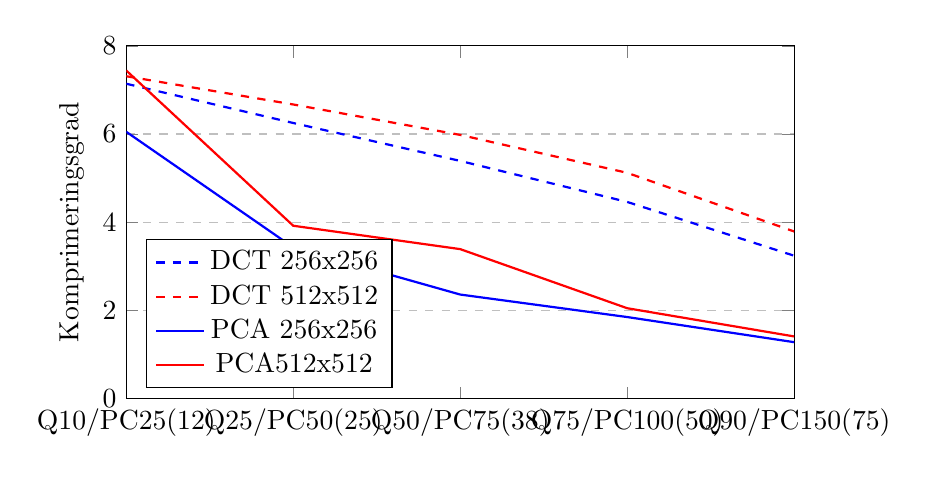
\begin{tikzpicture}
\begin{axis}[
%    title={Komprimering af skaleret billede},
    xlabel={},
    ylabel={Komprimeringsgrad},
    width = 0.83*\textwidth,
    height = 0.5*\textwidth,
    xtick = {0,1,2,3,4},
    xmin=0, xmax=4,
    ymin=0, ymax=8,
    %x tick label style = {anchor = east},
    xticklabels={Q10/PC25(12),Q25/PC50(25),Q50/PC75(38),Q75/PC100(50),Q90/PC150(75)},
    ytick={},
    legend pos=south west,
%    legend style={
%                at={(0,0)}},
    ymajorgrids=true,
    grid style=dashed,
]
 
\addplot[
    color=blue,
    dashed,
    thick,
    ]
    coordinates {
    (0,7.14)(1,6.25)(2,5.39)(3,4.46)(4,3.24)
    };
\addplot[
    color=red,
    dashed,
    thick,
    ]
    coordinates {
    (0,7.31)(1,6.67)(2,5.98)(3,5.12)(4,3.79)
    };
\addplot[
    color=blue,
    thick,
    ]
    coordinates {
    (0,6.05)(1,3.43)(2,2.36)(3,1.85)(4,1.28)
    };
\addplot[
    color=red,
    thick,
    ]
    coordinates {
    (0,7.44)(1,3.92)(2,3.39)(3,2.05)(4,1.41)
    };
]
\legend{DCT 256x256,DCT 512x512, PCA 256x256, PCA512x512}
\end {axis}
\end{tikzpicture}
\caption{Komprimeringsgrad for DCT og PCA ved skaleret Lena}
\label{fig:SkaleringLena-Komprimering}
\end{figure}

\begin{figure}[htbp]
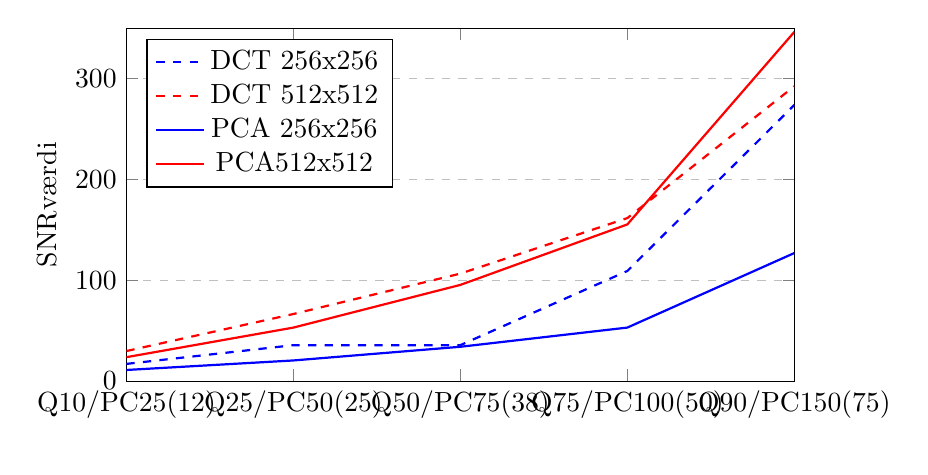
\begin{tikzpicture}
\begin{axis}[
%    title={SNR-værdier af skaleret billede},
    xlabel={},
    ylabel={SNRværdi},
    width = 0.83*\textwidth,
    height = 0.5*\textwidth,
    xtick = {0,1,2,3,4},
    xmin=0, xmax=4,
    ymin=0, ymax=350,
    xticklabels={Q10/PC25(12),Q25/PC50(25),Q50/PC75(38),Q75/PC100(50),Q90/PC150(75)},
%    x tick label style={rotate=45},
    ytick={},
    legend pos=north west,
%    legend style={
%                at={(0,0)}},
    ymajorgrids=true,
    grid style=dashed,
]
 
\addplot[
    color=blue,
    dashed,
    thick,
    ]
    coordinates {
    (0,17.02)(1,35.60)(2,35.61)(3,109.19)(4,273.85)
    };
\addplot[
    color=red,
    dashed,
    thick,
    ]
    coordinates {
    (0,29.77)(1,66.51)(2,106.58)(3,161.64)(4,292.41)
    };
\addplot[
    color=blue,
    thick,
    ]
    coordinates {
    (0,10.99)(1,20.44)(2,34.01)(3,53.05)(4,126.98)
    };
\addplot[
    color=red,
    thick,
    ]
    coordinates {
    (0,23.68)(1,53.04)(2,95.39)(3,155.38)(4,346.31)
    };
]
\legend{DCT 256x256,DCT 512x512, PCA 256x256, PCA512x512}
\end{axis}
\end{tikzpicture}
\caption{SNR-værdier for DCT og PCA ved skaleret Lena}
\label{fig:SkaleringLena-SNR}
\end{figure}

\section{Vurdering af mobilbilleder}
%Intro til afsnit
%Hvorfor giver mobilbilleder mening
%Hvilke præmisser er der (ny størrelse, billede, osv.)
%Hvordan komprimereres de (hvilke PCA og Q), hvorfor
%Resultater (hvorfor ingen gennemsnit osv.)
%Bekræfter ovenstående test, vores konklusion på baggrund af lena?
Det forsøges, at generalisere konklusionen fra foregående afsnit, der i sin essens lød, at de to komprimeringsmetoder var lige gode ved lave komprimeringskvaliteter, mens DCT var betydeligt bedre ved højere kvaliteter. For at kunne generalisere denne konklusion vil seks forskellige billeder blive taget med en mobiltelefon (noteret som T1, T2, …, T6), og vist i figur \ref{fig:T1} til \ref{fig:T6}. Disse billeder vil blive komprimeret med de to metoder, og ved hhv. en lav, mellem og høj komprimeringskvalitet for at sammenligne resultaterne.

\begin{figure}[!h]
\begin{minipage}[b]{0.3\linewidth}
\centering
\includegraphics[width=\textwidth]{Billeder/test_billeder/T1.jpg}
\caption{\href{https://www.dropbox.com/home/P1\%20-\%20B205/vejleder/billeder/Mobilbilleder/T1?preview=T1.jpg}{Mobilbillede \phantom{m} T1}}
\label{fig:T1}
\end{minipage}
\hspace{0.5cm}
\begin{minipage}[b]{0.3\linewidth}
\centering
\includegraphics[width=\textwidth]{Billeder/test_billeder/T2.jpg}
\caption{\href{https://www.dropbox.com/home/P1\%20-\%20B205/vejleder/billeder/Mobilbilleder/T2?preview=T2.jpg}{Mobilbillede T2}}
\label{fig:T2}
\end{minipage}
\hspace{0.5cm}
\begin{minipage}[b]{0.3\linewidth}
\centering
\includegraphics[width=\textwidth]{Billeder/test_billeder/T3.jpg}
\caption{\href{https://www.dropbox.com/home/P1\%20-\%20B205/vejleder/billeder/Mobilbilleder/T3?preview=T3.jpg}{Mobilbillede T3}}
\label{fig:T3}
\end{minipage}
\end{figure}

\begin{figure}[!h]
\begin{minipage}[b]{0.3\linewidth}
\centering
\includegraphics[width=\textwidth]{Billeder/test_billeder/T4.jpg}
\caption{\href{https://www.dropbox.com/home/P1\%20-\%20B205/vejleder/billeder/Mobilbilleder/T4?preview=T4.jpg}{Mobilbillede T4}}
\label{fig:T4}
\end{minipage}
\hspace{0.5cm}
\begin{minipage}[b]{0.3\linewidth}
\centering
\includegraphics[width=\textwidth]{Billeder/test_billeder/T5.jpg}
\caption{\href{https://www.dropbox.com/home/P1\%20-\%20B205/vejleder/billeder/Mobilbilleder/T5?preview=T5.jpg}{Mobilbillede T5}}
\label{fig:T5}
\end{minipage}
\hspace{0.5cm}
\begin{minipage}[b]{0.3\linewidth}
\centering
\includegraphics[width=\textwidth]{Billeder/test_billeder/T6.jpg}
\caption{\href{https://www.dropbox.com/home/P1\%20-\%20B205/vejleder/billeder/Mobilbilleder/T6?preview=T6.jpg}{Mobilbillede T6}}
\label{fig:T6}
\end{minipage}
\end{figure}

Billederne er taget i en opløsning på $2448 \times 3264$ pixels, hvilket er væsentligt større end Lena med dimensionerne $512 \times 512$ pixels. De specifikke komprimeringskvaliteter for DCT og PCA er valgt ud fra resultaterne med Lena.\\
Der er valgt tre par af komprimeringer, der udtrykker hhv. en lav, mellem og høj komprimeringskvalitet. Disse er bestemt til at være Q10, Q50 og Q90. PC25, PC75 og PC150 har tilnærmelsesvis samme SNR som disse ved komprimering af Lena, så disse vælges på baggrund af dette. Da mobilbillederne, som der undersøges med herunder, er langt større, skaleres antallet af principale komponenter op, så det passer til størrelsen af billederne. Dette betyder, at parrene kommer til se således ud
\begin{itemize}
	\item[]{Q10 og PC120}
	\item[]{Q50 og PC360}
	\item[]{Q90 og PC720}
\end{itemize}
For hvert af parrene sammenlignes SNR og komprimeringsgrad. I figur \ref{fig:mobilbilleder_SNR} ses grafer for SNR for  begge metoder med alle billederne. På samme måde illustrerer figur \ref{fig:mobilbilleder_komprimering} grafer for komprimeringsgraderne. Desuden er der inkluderet en graf for komprimering af Lena udført med Q10, Q50, Q90 og PC25, PC75 og PC150 for sammenligning.
\definecolor{dblue}{HTML}{0000CC}
%\definecolor{lblue}{HTML}{6666FF}
\definecolor{dgreen}{HTML}{006600}
%\definecolor{lgreen}{HTML}{329932}
\definecolor{dred}{HTML}{CC0000}
%\definecolor{lred}{HTML}{FF6666}
\definecolor{dturquoise}{HTML}{2C9C91}
%\definecolor{lturquoise}{HTML}{79E9DE}
\definecolor{dpurple}{HTML}{660066}
%\definecolor{lpurple}{HTML}{A64CA6}
\definecolor{dorange}{HTML}{CC8400}
%\definecolor{lorange}{HTML}{FFB732}
\begin{figure}
\begin{tikzpicture}
\begin{axis}[
%    title={SNR-værdi ved komprimering af mobilbilleder},
    xlabel={},
    ylabel={SNR-værdi},
    width = 0.83*\textwidth,
    height = 9cm,
    xtick = {0,1,2},
    xmin=0, xmax=2,
    ymin=0, ymax=3500,
    y tick label style={
        /pgf/number format/.cd,
       		use comma,
        	/tikz/.cd},
    %x tick label style = {anchor = east},
    xticklabels={Q10/PC120(25),Q50/PC360(75),Q90/PC720(150)},
    ytick={},
    legend pos=south east,
    legend style={
                at={(1.25,0)}},
    ymajorgrids=true,
    grid style=dashed,
]
 
\addplot[
    color=dblue,
    dashed,
    thick,
    ]
    coordinates {
    (0,111.36)(1,581.01)(2,2145.30)
    };
\addplot[
    color=dblue,
    thick,
    ]
    coordinates {
    (0,190.95)(1,791.52)(2,2914.51)
    };
\addplot[
    color=dgreen,
    dashed,
    thick,
    ]
    coordinates {
    (0,111.36)(1,581.01)(2,1817.41)
    };
\addplot[
    color=dgreen,
    thick,
    ]
    coordinates {
    (0,730.56)(1,1350.62)(2,3056.68)
    };
\addplot[
    color=dred,
    dashed,
    thick,
    ]
    coordinates {
    (0,41.72)(1,307.30)(2,958.41)
    };
\addplot[
    color=dred,
    thick,
    ]
    coordinates {
    (0,165.83)(1,639.55)(2,1581.68)
    };
\addplot[
    color=dturquoise,
    dashed,
    thick,
    ]
    coordinates {
    (0,62.54)(1,383.17)(2,1608.79)
    };
\addplot[
    color=dturquoise,
    thick,
    ]
    coordinates {
    (0,110.57)(1,509.59)(2,1712.87)
    };
\addplot[
    color=dpurple,
    dashed,
    thick,
    ]
    coordinates {
    (0,56.44)(1,298.69)(2,1016.79)
    };
\addplot[
    color=dpurple,
    thick,
    ]
    coordinates {
    (0,53.10)(1,238.69)(2,978.65)
    };
\addplot[
    color=dorange,
    dashed,
    thick,
    ]
    coordinates {
    (0,59.80)(1,279.01)(2,918.94)
    };
\addplot[
    color=dorange,
    thick,
    ]
    coordinates {
    (0,55.94)(1,226.80)(2,819.59)
    };
    \addplot[
    color=black,
    dashed,
    thick,
    ]
    coordinates {
    (0,59.80)(1,279.01)(2,918.94)
    };
\addplot[
    color=black,
    thick,
    ]
    coordinates {
    (0,29.77)(1,106.58)(2,292.41)
    };
	\legend{T1DCT, T1PCA, T2DCT, T2PCA, T3DCT, T3PCA, T4DCT, T4PCA, T5DCT, T5PCA, T6DCT, T6PCA, LenaDCT, LenaPCA}
\end{axis}
\end{tikzpicture}
\caption{SNR-værdier for mobilbilleder}
\label{fig:mobilbilleder_SNR}
\end{figure}

\begin{figure}
\begin{tikzpicture}
\begin{axis}[
%    title={Komprimeringsgrad af mobilbilleder},
    xlabel={},
    ylabel={Komprimeringsgrad},
    width = 0.83*\textwidth,
    height= 9cm,
    xtick = {0,1,2},
    xmin=0, xmax=2,
    ymin=0, ymax=12,
    %x tick label style = {anchor = east},
    xticklabels={Q10/PC120(25),Q50/PC360(75),Q90/PC720(150)},
    ytick={},
    legend pos=south east,
    legend style={
                at={(1.25,0)}},
    ymajorgrids=true,
    grid style=dashed,
]
 
\addplot[
    color=dblue,
    dashed,
    thick,
    ]
    coordinates {
    (0,7.42)(1,6.62)(2,4.84)
    };
\addplot[
    color=dblue,
    thick,
    ]
    coordinates {
    (0,10.30)(1,3.64)(2,1.91)
    };
\addplot[
    color=dgreen,
    dashed,
    thick,
    ]
    coordinates {
    (0,7.56)(1,7.15)(2,5.37)
    };
\addplot[
    color=dgreen,
    thick,
    ]
    coordinates {
    (0,11.60)(1,4.04)(2,2.08)
    };
\addplot[
    color=dred,
    dashed,
    thick,
    ]
    coordinates {
    (0,7.62)(1,7.06)(2,5.61)
    };
\addplot[
    color=dred,
    thick,
    ]
    coordinates {
    (0,10.30)(1,3.79)(2,2.02)
    };
\addplot[
    color=dturquoise,
    dashed,
    thick,
    ]
    coordinates {
    (0,7.49)(1,6.80)(2,4.94)
    };
\addplot[
    color=dturquoise,
    thick,
    ]
    coordinates {
    (0,10.00)(1,3.61)(2,1.91)
    };
\addplot[
    color=dpurple,
    dashed,
    thick,
    ]
    coordinates {
    (0,7.36)(1,6.31)(2,4.35)
    };
\addplot[
    color=dpurple,
    thick,
    ]
    coordinates {
    (0,9.75)(1,3.48)(2,1.83)
    };
\addplot[
    color=dorange,
    dashed,
    thick,
    ]
    coordinates {
    (0,7.47)(1,6.63)(2,4.78)
    };
\addplot[
    color=dorange,
    thick,
    ]
    coordinates {
    (0,9.90)(1,3.53)(2,1.85)
    };
   	    \addplot[
    color=black,
    dashed,
    thick,
    ]
    coordinates {
    (0,7.31)(1,5.98)(2,3.79)
    };
\addplot[
    color=black,
    thick,
    ]
    coordinates {
    (0,7.44)(1,3.39)(2,1.41)
    };
	\legend{T1DCT, T1PCA, T2DCT, T2PCA, T3DCT, T3PCA, T4DCT, T4PCA, T5DCT, T5PCA, T6DCT, T6PCA, LenaDCT, LenaPCA}
\end{axis}
\end{tikzpicture}
\caption{Komprimgeringsgrad af mobilbilleder}
\label{fig:mobilbilleder_komprimering}
\end{figure}

\subsubsection{Q10 og PC120}
Det ses af grafen i figur \ref{fig:mobilbilleder_SNR}, at PC120 opnår højere SNR for billede T1, T2 og T3, end DCT gør. Dette skyldes formentlig, at disse billeder indeholder få bratte ændringer - de består af mange glatte overgange, og PCA kan derfor let udtrykke meget af billedet ved få principale komponenter. DCT med Q10 opnår mindre støj i T5 og T6, hvilket er en følge af, at der er flere forskellige farver i disse billeder. For T4 opnås ca. samme SNR for de to metoder.
Det ses desuden på grafen i figur \ref{fig:mobilbilleder_komprimering}, at PC120 tilmed opnår en højere komprimeringsgrad end DCT ved Q10.\\
På papiret er PC120 bedre end Q10, men i praksis bruges disse komprimeringsgrader sjældent, da de laver billeder af en uønskværdig kvalitet.

\subsubsection{Q50 og PC360}
Det ses af grafen i figur \ref{fig:mobilbilleder_SNR}, at PCA ved PC360 stadig opnår bedre SNR end DCT med Q50 for billede T1, T2 og T3. Resultaterne for sammenligningen af SNR er tilmed magen til dem for Q10 og PC120 for de resterende billeder. Det ses dog på grafen i figur \ref{fig:mobilbilleder_komprimering}, at Q50 opnår væsentligt bedre komprimering end PC360 for alle seks billeder.

\subsubsection{Q90 og PC720}
Sammenligningen af Q90 og PC720 har samme grundlæggende tendenser som den ovenstående - PCA giver for T1, T2 og T3 bedre billedkvalitet end DCT, mens DCT håndterer T5 og T6 bedre. De opnår lignende resultater for T4. DCT opnår dog imidlertid langt højere komprimeringsgrad end PCA gør og billederne fylder dermed mindre, hvilket er ønskværdigt.\\
Bemærk, at DCT opnår både bedre SNR og komprimeringsgrad for alle par ved komprimering af Lena.

\subsubsection{Delkonklusion - mobilbilleder}
Komprimering af mobilbillederne giver anderledes resultater, end komprimering af Lena gør. Ikke desto mindre opnår PCA stadig ringere komprimering end DCT ved højere kvaliteter. Dette ses dog i lyset at, at PCA opnår bedre SNR. PCA håndterer altså mobilbillederne bedre end den håndterer Lena.\\
At PCA er bedre ved lave kvaliteter er nær ubrugeligt, da det ikke er interessant at se på ringe kvaliteter - dette er derfor en negligerbar egenskab. DCT indgår et mere ønskværdigt kompromis med kvaliteten for højere komprimeringsgrad - mobilbilleder skal komprimeres meget og bibeholde kvaliteten. DCT må derfor siges at være bedre end PCA til komprimering af mobilbilleder.

%Det fremkommer i disse resultater at PCA gennemgående er bedre til at komprimere ved den lave kvalitet. Her giver PCA bedre SNR-værdi, såvel som højere komprimeringsgrad. Dette skyldes at PCA bruger de første få komponenter til at udtrykke en stor del af billedet, hvorved det meget hurtigt kan skabe en tilnærmelse af billedet, og de resterende komponenter udtrykker "blot" \ detaljer i billedet, der ikke har stor betydning for det samlede resultat. Derudover komprimerer PCA meget godt, når den kun bruger få komponenter. Dette ses også i tabel \ref{tb:komprimering_PCA1} og \vref{tb:komprimering_PCA2}. Det skal dog bemærkes, at der ved T2 og T3 er betydeligt bedre SNR-værdier med PCA end DCT, hvilket skyldes den store ensformighed i billederne, hvilket gør at PCA fungerer bedre.\\
%Når kvaliteten øges til mellem kvalitet ($Q50$ og $PCA360$), ses der gennemgående et udsving i resultaterne, hvor komprimeringsgraden for PCA falder betydeligt i forhold til DCT. Ligesom med Lena er det gennemgående, at DCT holder en nogenlunde stabil komprimeringsgrad på tværs af kvaliteterne, hvor PCA har et større udsving i komprimeringsgraden. Dette illustrerer figur \ref{fig:mobilbilleder_komprimering} også, hvor den generelle hældning for PCA-komprimeringerne er højere end for DCT.\\
%Undersøges resultaterne ved den høje komprimeringskvalitet ($Q90$ og $PCA720$) bliver det igen tydeligt, at der er forskel på billederne der arbejdes med. PCA-komprimeringerne af T2 og T3 giver betydeligt bedre SNR-værdier end DCT, men har også betragteligt lavere komprimeringsgrader. Dette skyldes at T2 og T3 er meget ensformige, og ved en høj kvalitet har PCA nok principale komponenter til at repræsentere detaljer og derved forbedre SNR-værdien. Da DCT ikke tilpasser sig dataene den transformerer, vil denne ikke være i stand til i samme grad at tage højde for den store ensformighed.\\
%I modsætning til Lena-billedet ved forholdsvist mange principale komponenter og en kvantiseringstabel på $Q90$, ses det at ved T4, T5 og T6 ligger SNR-værdierne tæt på hinanden. Det kan skyldes den enorme forskellighed i billedet, hvor PCA og DCT i og for sig udligner hinanden ved styrker og svagheder forskellige steder på billedet. Det fremgår dog klart at DCT stadig er langt mere effektiv til at komprimere ved høj billedkvalitet.
%Endvidere hvis resultaterne vurderes subjektivt, ses det ligesom den objektive vurdering, at PCA fungerer bedre ved ensformige billeder, da den ikke behøver mange principale komponenter for at udtrykke hele billedet - T2 er et glimrende eksempel på dette. Modsat et meget kontrastfyldt billede, dvs. med mange ændringer, skal PCA bruge enormt mange principale komponenter for at udtrykke små ændringer i billedet. I dette tilfælde vil DCT give bedre resultater, da den blot udglatter de små ændringer - T6 kunne være et eksempel på dette. \fxnote{Lineær komprimeringsgrad for PCA - skal flettes ind i teksten på et tidspunkt}

\section{Fejlkilder}
I forbindelse med brug af hhv. DCT og PCA til komprimering af billeder er der nogle begrænsninger og fejlkilder, som påvirker resultatet. Det følgende afsnit vil præsentere disse fejlkilder, såvel som den indflydelse de har på resultaterne.

\subsubsection{DCT fejlkilder}
Den diskrete cosinustransformation fungerer i billedkomprimeringsalgoritmer, fordi den energikomprimerer et signal effektivt. Dette er imidlertid kun tilfældet, når signalet er glat. Når der snakkes om billeder, vil det sige, at farveintensiteter i alle $8 \times 8$ matricer er relativt ens, eller udtrykker en glat overgang. Hvis billedet ikke har denne egenskab, skal transformationen bruge mange cosinusfunktioner til at udtrykke billedet, og der vil ikke blive opnået en god energikomprimering. Er der derfor mange bratte ændringer i billedet, vil det resultere i at DCT ikke vil være i stand til at komprimere så godt. \\
Netop fordi at DCT bygger på cosinustransformationer, der er svingninger, har denne metode også problemer med at udtrykke bratte ændringer korrekt. Med de 64 cosinusfunktioner (se ligning \vref{eq:DCTeq}, hvor $n=8$), der bruges i denne transformation (hvoraf dem med højeste frekvens ofte fjernes i kvantiseringen og afrundingen), er det ikke muligt at repræsentere bratte ændringer godt. Dette resulterer i at der omkring kanter, hvor der er stor ændring, typisk opstår større fejl og unøjagtigheder end i andre dele af billedet.

DCT fungerer på $8 \times 8$ matricer, men såfremt et billedes dimensioner ikke kan divideres med otte, vil den sidste matrix ikke indeholde tilstrækkelige data til at udfylde alle indgange. Der er to mulige løsninger til problemet: ikke at komprimere den yderste kant (op til syv pixels) af billedet eller at nulfylde kanten, så billeddimensionerne går op i otte [\citet{zero_padding}, s. 1]. Komprimeres kanten ikke vil det give en dårligere komprimeringsgrad, da tallene ikke vil blive centreret omkring nul, og Huffmankodningen vil derfor ikke fungere optimalt i disse kanter. Nulfyldes kanten, hvilket svarer til at lave en grå kant, vil der i mange billeder opstå en brat ændring mellem billedet og kanten, hvilket vil have betydning for komprimeringen af kanten, såvel som at det dekomprimerede billede vil være påvirket af den grå kant jævnfør tidligere fejlkilder.
%En alternativ løsning kunne være at fylde de resterende pixels med en spejling af de yderste pixels. Dette vil betyde at den tilføjede kant ligner de pixels der ligger ud til kanten. Dette kan dog give fejl, hvis de pixels der spejles ud i kanten repræsenterer en brat kontrast. Dette vil resultere i at kontrasten fremgår to gange. I mange tilfælde, må det dog kunne forventes at kunne give et bedre resultat end en nulfyldning.

\subsubsection{PCA fejlkilder}
PCA bruges normalt til reducering af dimensioner på store datasæt og for at finde sammenhænge, der ikke nødvendigvis er tydelige, når der kigges på dataene. PCA reducerer herved dimensionerne til de mest betydende, og derved kan store dimensioner af data nedbringes til få betydende dimensioner. Det er ikke helt samme præmis, der er i spil, når PCA bliver brugt som billedekomprimeringsmetode. Her er der ikke nødvendigvis samme sammenhæng mellem de enkelte rækker af pixels, som der er mellem målinger i et datasæt, som PCA normalvis bruges på. Dette betyder, at PCA fungerer godt til at reducere dimensionerne meget, men dette resulterer ikke nødvendigvis i gode resultater visuelt. Det betyder også, at når PCA ikke reducerer dimensionerne meget, men bibeholder en betydelig mængde principale komponenter, så ændrer kvaliteten sig ikke meget, men komprimeringsgraden falder. PCA er altså ikke beregnet til billedkomprimering, men kan med acceptable resultater bruges til det.

Når det komprimerede billede gemmes til en fil, opstår der en fejlkilde. For at få sammenlignelige data bruges Huffmankodning også på PCA, men for at denne metode giver mening, skal tallene, der gemmes, være heltal. Dette er problematisk, da egenvektorerne i $P$ er ortonormale, hvorved alle indgange er meget små for tilsammen at give en længde på én. Dette gør, at en afrunding fuldstændigt eliminerer nærmest samtlige værdier i $P$. Ved at multiplicere alle indgangene med 10.000 inden de afrundes og Huffmankodes, opnåes heltal på op til fire cifre. Tallene divideres blot med 10.000 i dekodningen, og afrundingen, der før ændrede alle indgange til nul, afrunder nu blot på det, der svarer til femte decimal. Dette ændrer på dataene, der i dekomprimeringen ikke bliver de eksakt samme, men der kan ses bort fra fejlene fremkommet ved denne afrunding, da disse anses som ubetydeligt små.

\subsubsection{Generelle fejlkilder}
Når de komprimerede billeder dekomprimeres, sker det, at de dekomprimerede pixelværdier afviger fra de tilladte værdier $0 \leq \text{pixelværdi} \leq 255$. Dette skyldes afrundingen af tallene i forbindelse med, at filerne bliver gemt med Huffmankodning. Dette betyder imidlertid, at alle tal under nul trunkeres til at være nul og alle tal over 255 til 255. Dette er dog i meget få tilfælde nødvendigt og er typisk tal, der i forvejen ville være endt på 255. Der vil altså ikke være en visuel tydelig forskel ved denne ændring.

Den subjektive vurdering af billedkvalitet er netop subjektiv, og det kan ikke regnes med, at denne siger noget endegyldigt om komprimeringsteknikkerne, med mindre det bakkes op af statistiske beviser i form af store datasæt fra store empiriske undersøgelser.
I denne rapport er det kun gruppemedlemmerne, der har vurderet subjektivt på billederne, derfor kan der ikke siges at være statistisk belæg for konklusionerne, hvorved de blot bør anses som bemærkninger/suppleringer til den objektive vurdering.

I forbindelse med generaliseringen af delkonklusionen, der er udformet på baggrund af resultater med komprimering af Lena, sammensættes par af Q-værdier og antal principale komponenter, for at have ensformige data at vurdere på ved mobilbillederne. Disse par er dog sammensat på baggrund af metodernes effektivitet på Lena og ved andre billeder, kan disse par vise sig at være misvisende og ikke give udtryk for samme kvalitet, som de oprindeligt var udvalgt til. Denne pardannelse antages at give et nogenlunde grundlag for sammenligning.
%%\begin{tikzpicture}
%\begin{axis}[
%    title={SNR-værdier af scaleret billede},
%    xlabel={},
%    ylabel={SNRværdi},
%    width = 0.83*\textwidth,
%    height = 0.5*\textwidth,
%    xtick = {0,1,2,3,4},
%    xmin=0, xmax=4,
%    ymin=0, ymax=8,
%    %x tick label style = {anchor = east},
%    xticklabels={Q10/PC25(12),Q25/PC50(25),Q50/PC75(38),Q75/PC100(50),Q90/PC150(75)},
%    ytick={},
%    legend pos=south east,
%    legend style={
%                at={(1.23,0)}},
%    ymajorgrids=true,
%    grid style=dashed,
%]
% 
%\addplot[
%    color=blue,
%    dashed,
%    ]
%    coordinates {
%    (0,17.02)(1,35.60)(2,35.61)(3,109.19)(4,273.85)
%    };
%\addplot[
%    color=red,
%    dashed,
%    ]
%    coordinates {
%    (0,29.77)(1,66.51)(2,106.58)(3,161.64)(4,292.41)
%    };
%\addplot[
%    color=blue,
%    ]
%    coordinates {
%    (0,10.99)(1,20.44)(2,34.01)(3,53.05)(4,126.98)
%    };
%\addplot[
%    color=red,
%    ]
%    coordinates {
%    (0,23.68)(1,53.04)(2,95.39)(3,155.38)(346.31)
%    };
%]
%\legend{DCT 256x256,DCT 512x512, PCA 256x256, PCA512x512}
%\end {axis}
%\end{tikzpicture}

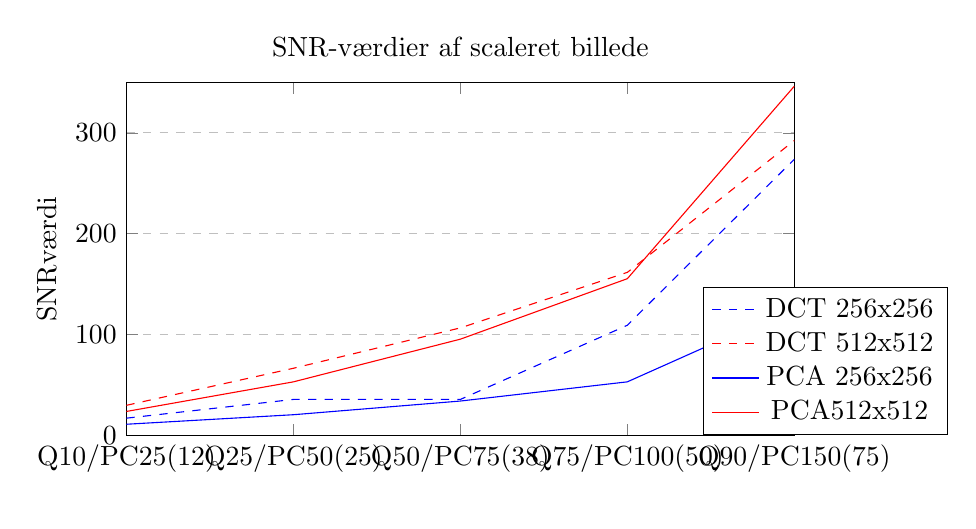
\begin{tikzpicture}
\begin{axis}[
    title={SNR-værdier af scaleret billede},
    xlabel={},
    ylabel={SNRværdi},
    width = 0.83*\textwidth,
    height = 0.5*\textwidth,
    xtick = {0,1,2,3,4},
    xmin=0, xmax=4,
    ymin=0, ymax=350,
    %x tick label style = {anchor = east},
    xticklabels={Q10/PC25(12),Q25/PC50(25),Q50/PC75(38),Q75/PC100(50),Q90/PC150(75)},
    ytick={},
    legend pos=south east,
    legend style={
                at={(1.23,0)}},
    ymajorgrids=true,
    grid style=dashed,
]
 
\addplot[
    color=blue,
    dashed,
    ]
    coordinates {
    (0,17.02)(1,35.60)(2,35.61)(3,109.19)(4,273.85)
    };
\addplot[
    color=red,
    dashed,
    ]
    coordinates {
    (0,29.77)(1,66.51)(2,106.58)(3,161.64)(4,292.41)
    };
\addplot[
    color=blue,
    ]
    coordinates {
    (0,10.99)(1,20.44)(2,34.01)(3,53.05)(4,126.98)
    };
\addplot[
    color=red,
    ]
    coordinates {
    (0,23.68)(1,53.04)(2,95.39)(3,155.38)(4,346.31)
    };
]
\legend{DCT 256x256,DCT 512x512, PCA 256x256, PCA512x512}
\end{axis}
\end{tikzpicture}


%\definecolor{dblue}{HTML}{0000CC}
%\definecolor{lblue}{HTML}{6666FF}
%\definecolor{dgreen}{HTML}{006600}
%\definecolor{lgreen}{HTML}{329932}
%\definecolor{dred}{HTML}{CC0000}
%\definecolor{lred}{HTML}{FF6666}
%\definecolor{dturquoise}{HTML}{2C9C91}
%\definecolor{lturquoise}{HTML}{79E9DE}
%\definecolor{dpurple}{HTML}{660066}
%\definecolor{lpurple}{HTML}{A64CA6}
%\definecolor{dorange}{HTML}{CC8400}
%\definecolor{lorange}{HTML}{FFB732}
%
%\begin{tikzpicture}
%    \begin{axis}[
%        width  = 0.85*\textwidth,
%        height = 8cm,
%        major x tick style = transparent,
%        ymajorgrids = true,
%        xmajorgrids=true,
%    		grid style=dashed,
%        ylabel = {Procent (\%)},
%		xlabel = {Principal Komponenter},
%        ymin=0,
%%		tick style={line width=5pt}
%        legend cell align=left,
%        legend style={
%                at={(0.12,-0.15)},
%                anchor=north west,
%                legend columns= -1,
%                /tikz/every even column/.append style= {column sep=1.0cm}}
%    ]
%        \addplot [ultra thick, dblue] table [col sep=comma, mark = none] {Formalia/Data/T1Q.xlsx};
%        \addplot [ultra thick, lblue] table [col sep=comma, mark = none] {Formalia/Data/T1PCA.xlsx};
%		\addplot [ultra thick, dgreen] table [col sep=comma, mark = none] {Formalia/Data/T2Q.xlsx};
%		\addplot [ultra thick, lgreen] table [col sep=comma, mark = none] {Formalia/Data/T2PCA.xlsx};
%		\addplot [ultra thick, dred] table [col sep=comma, mark = none] {Formalia/Data/T3Q.xlsx};
%		\addplot [ultra thick, lred] table [col sep=comma, mark = none] {Formalia/Data/T3PCA.xlsx};
%		\addplot [ultra thick, dturquoise] table [col sep=comma, mark = none] {Formalia/Data/T4Q.xlsx};
%		\addplot [ultra thick, lturquoise] table [col sep=comma, mark = none] {Formalia/Data/T4PCA.xlsx};
%		\addplot [ultra thick, dpurple] table [col sep=comma, mark = none] {Formalia/Data/T5Q.xlsx};
%		\addplot [ultra thick, lpurple] table [col sep=comma, mark = none] {Formalia/Data/T5PCA.xlsx};
%		\addplot [ultra thick, dorange] table [col sep=comma, mark = none] {Formalia/Data/T6Q.xlsx};
%		\addplot [ultra thick, lorange] table [col sep=comma, mark = none] {Formalia/Data/T6PCA.xlsx};
%%        \legend{Rød, Grøn, Blå , Samlet}
%    \end{axis}
%\label{fig:PCAdiagram}
%\end{tikzpicture}

\chapter{Konklusion}
Følgende afsnit har til formål at konkludere på projektet og de brugte metoder i relation til den opstillede case.

De to billedkomprimeringsteknikker udarbejdet i rapporten bygger på to forskellige matematiske værktøjer - en diskret cosinustransformation og principalkomponentanalyse af et billede beregnet med brug af egenværdier. DCT udtrykker et signal som en sum af cosinusfunktioner og giver dermed et indblik i, hvordan signalet er bygget op. Når der ses på billeder, kan transformationen bruges til at identificere, hvilke informationer om billedet som er (næsten) redundante - disse kan dermed fjernes, og billedet kan komprimeres. PCA beregner egenvektorer for billedet og benytter de mest betydende af disse til at udtrykke billedet - disse hedder principale komponenter.

Det fremkom ved sammenligning af de behandlede Lena, at DCT, ved den samme komprimeringsgrad som PCA, gav et pænere billede, hvilket blev underbygget både objektivt af SNR og subjektivt.
Der kan desuden konkluderes, at både DCT og PCA bliver påvirket af dimensionerne af et billede - mindre billeder giver ringere resultater for begge metoder, mens større billeder giver bedre resultater. Dette ændrer ikke på, hvordan de komprimerer i forhold til hinanden - DCT er stadig bedre end PCA.

PCA kan opnå langt flere komprimeringsgrader end DCT og er derfor mere fleksibel. Dette skyldes, at PCA oprindeligt er udviklet til at finde en sammenhæng i et datasæt og beskrive det med så få sammenhængende prinicipale komponenter som muligt. Denne egenskab er dog ikke optimal, når et billede skal komprimeres, da hele billedet gerne skal beskrives så nøjagtigt som muligt. Dette gør, at der skal bruges et højere antal principale komponenter, end metoden var tiltænkt, for at billedet stadig kan beskrives, så det ikke er til gene for brugeren. Metoden kan med fordel bruges på billeder, som er meget ensartede, som det kan ses på resultaterne af T2. Men det er DCT, der ved subjektiv vurdering skaber det bedste billede set på resten af testbillederne. 
DCT er ikke i stand til at opnå samme komprimeringsgrad som PCA, men måden hvorpå den fjerner de høje frekvenser fra billedet, som til en hvis grad er overflødige, betyder at den ofte danner de pæneste billeder, hvis komprimeringsgraden holdes ens med PCA.

Da formålet med rapporten er, at undersøge hvilken af de to komprimeringsalgoritmer, som bedst kunne bruges til komprimering af billeder taget med og lagret på en mobil, er det ønskværdigt at bevare billedkvaliteten i samspil med en høj komprimeringsgrad. Ud af de to metoder, PCA og DCT, viser DCT sig at være den bedste i tilfælde, hvor billedet ikke har mange glatte overgang over det hele - den er langt mere alsidig end PCA, der primært håndterer meget ensformige billeder godt.

Det kan derfor konkluderes, at komprimeringsalgoritmen, som bygger på en diskret cosinustransformation, er den bedste løsning til komprimering af billeder på en mobiltelefon i forhold til PCA.

\section{Perspektivering}
Dette projekt har været begrænset til billedkomprimering med en diskret cosinustransformation og principale komponenter i et billede. Der findes mange andre komprimeringsmetoder, tabsfri såvel som ikke-tabsfri, som ikke er undersøgt i denne rapport. I dette afsnit overvejes nogle af mulighederne, som kunne have været relevante for projektet, men som ikke er inkluderet.

\textbf{DCT}\\
Der findes andre transformationer end en diskret cosinustransformation, som kan benyttes i en billedkomprimeringsalgoritme. Blandt disse kan nævnes
\begin{itemize}
	\item[]{\textit{Diskret Fouriertransformation} (DFT)\\
	som allerede er blevet omtalt. Transformationen er DCT underlegen i forbindelse med billedkomprimering.}\\
	\item[]{\textit{Diskret Sinustransformation} (DST)\\
	som udtrykker et singal ved sinusfunktioner, men som ikke opnår lige så høj energikomprimering af billeder som DCT.}\\
	\item[]{\textit{Diskret Wavelettransformation} (DWT)\\
	som indgår i den nye og forbedrede JPEG-algoritme, JPEG2000. Transformationen er DCT overlegen og kan tilmed udføre tabsfri komprimering.}
\end{itemize}

\textbf{PCA}\\
Som tidligere bemærket kan PCA bruges til meget andet end billedkomprimering, hvor det er nyttigt at finde ligheder i store mængder data. En udbredt brug af PCA er inden for ansigtsgenkendelse, hvor ansigter udtrykkes som en sum af egenansigter komponeret af principale komponenter. Der kunne alternativt have været lavet egenansigter med PCA på DCT-komprimerede billeder, for at se hvordan komprimeringen påvirker PCAs funktionsdygtighed.

\textbf{Tabsfri}\\
I projektet benyttes Huffmankodning, som er en tabsfri komprimeringsmetode. Denne bruges dog ikke alene til billedkomprimering, og i projektet er der ikke undersøgt en, udelukkende, tabsfri billedkomprimeringsmetode. Det kunne være interessant at undersøge eller lave en tabsfri algoritme, for at kunne sammenligne de to typer på billedkvalitet og komprimeringsgrad. Blandt tabsfrie billedformater kan nævnes PNG og TIFF.

\textbf{Farverum}\\
I projektet undersøges farvebilleder efter RGB-farvemodellen, og komprimeringerne udføres ligeledes i denne opdeling af farverummene. Til billedkomprimering deles billeder ofte op i farverummene YCrCb (se afsnit \vref{sec:teori_intro}), da det med denne opdeling kan lade sig gøre at lave en mere effektiv komprimering grundet farverummenes egenskaber.
%\chapter{Perspektivering}
Dette projekt har været begrænset til billedkomprimering med en diskret cosinustransformation og principale komponenter i et billede. Der findes mange andre komprimeringsmetoder, tabsfri såvel som ikke-tabsfri, som ikke er undersøgt i denne rapport. I dette afsnit overvejes nogle af mulighederne, som kunne have været relevante for projektet, men som ikke er inkluderet.

\textbf{DCT}\\
Der findes andre transformationer end en diskret cosinustransformation, som kan benyttes i en billedkomprimeringsalgoritme. Blandt disse kan nævnes
\begin{itemize}
	\item[]{\textit{Diskret Fouriertransformation} (DFT)\\
	som allerede er blevet omtalt. Transformationen er DCT underlegen i forbindelse med billedkomprimering.}\\
	\item[]{\textit{Diskret Sinustransformation} (DST)\\
	som udtrykker et singal ved sinusfunktioner, men som ikke opnår lige så høj energikomprimering af billeder som DCT.}\\
	\item[]{\textit{Diskret Wavelettransformation} (DWT)\\
	som indgår i den nye og forbedrede JPEG-algoritme, JPEG2000. Transformationen er DCT overlegen og kan tilmed udføre tabsfri komprimering.}
\end{itemize}

\textbf{PCA}\\
Som tidligere bemærket kan PCA bruges til meget andet end billedkomprimering, hvor det er nyttigt at finde ligheder i store mængder data. En udbredt brug af PCA er inden for ansigtsgenkendelse, hvor ansigter udtrykkes som en sum af egenansigter komponeret af principale komponenter. Man kunne alternativt have lavet egenansigter med PCA på DCT-komprimerede billeder for at se hvordan komprimeringen påvirker PCAs funktionsdygtighed.

\textbf{Tabsfri}\\
I projektet benyttes Huffmankodning, som er en tabsfri komprimeringsmetode. Denne bruges dog ikke isoleret til billedkomprimering og i projektet er der ikke arbejdet med en udelukkende tabsfri billedkomprimeringsmetode. Det kunne være interessant at undersøge eller lave en tabsfri algoritme, for at kunne sammenligne de to typer på billedkvalitet og komprimeringsgrad. Blandt tabsfrie billedformater kan nævnes bl.a. PNG og TIFF.

\textbf{Farverum}\\
I projektet arbejdes med farvebilleder efter RGB-farvemodellen, og komprimeringerne udføres ligeledes i denne opdeling af farverummene. Til billedkomprimering deles billeder ofte op i farverummene YCrCb (se afsnit \vref{teori_intro}), da det med denne opdeling kan lade sig gøre at lave en mere effektiv komprimering grundet farverummenes egenskaber.


%%%% Kilder %%%%

\begingroup
	\raggedright
	\small\bibliography{Bibtex/Litteratur}						% Litteraturlisten inkluderes
\endgroup


%%%% Fixme-listen %%%%

%\newpage														% Ny side til Fixme-listen
%\listoffixmes													% Fixme-listen - fjernes til sidst i projektet med "%"


%%%% Appendiks %%%%

\appendix														% Appendiks/bilag start - giver chapter bogstaver i stedet for tal
\clearforchapter													% Sikrer at pagestylen aktiveres paa den rigtige side
\phantomsection													% Kunstigt afsnit, som hyperlinks kan 'holde fast i'
\pdfbookmark[0]{Appendiks}{appendiks}							% Tildeler en klikbar bookmark til den endelige PDF

%% Indstillinger for appendiks (deaktiveret med "%") %%

%\pagestyle{empty}												% Sidehoved/-fod for standardsider aendres til tom for appendiks
%\aliaspagestyle{chapter}{empty}								% Sidehoved/-fod for kapitelsider aendres til tom for appendiks
%\settocdepth{chapter}											% Kun kapitel-niveau vises i ToC
%\addtocontents{toc}{\protect\cftpagenumbersoff{chapter}}		% Sidetal for kapitler fjernes i ToC

%% Filer til appendiks %%

\chapter{DCT udledning}
\label{DCT_udledning}
I dette afsnit beskrives udledningen af DCT fra den diskrete Fouriertransformation med udgangspunkt i [\citet{applied_mathematics}, s. 179-183].

Lad $\vec{x}=[x_0,\ldots,x_{n-1}]^T \in \mathbb{R}^n$ og $\tilde{\vec{x}}=[\tilde{x}_0,\ldots,\tilde{x}_{2n-1}]^T \in \mathbb{R}^{2n}$ således at $\tilde{\vec{x}}$ er den forlængede $\vec{x}$, sådan at de er symmetrisk omkring $n-\frac{1}{2}$.

Definitionsmængden for $\tilde{x_l}$ er givet som
\begin{equation}
\tilde{x}_l = 
\begin{cases}
			x_l, \phantom{mmm} for \ l = 0,\ldots,n - 1 \\
			x_{2n-l-1},\ for \ l = n,\ldots,2n - 1
\end{cases}
\label{eq:x_tilde}
\end{equation}
Qua [\citet{applied_mathematics}, s. 174] er Fourier transformationen for en vektor $\vec{x} \in \mathbb{C}^n$ givet som
\begin{align}
\hat{\vec{x}}=F_n\vec{x}
\end{align}
og den $j$'te indgang af $\hat{\tilde{x}}$ er givet som
\begin{align}
\Big(\hat{\tilde{\vec{x}}}\Big)_j = \sum_{l=0}^{2n - 1} \tilde{x}_l \textit{e}^{-i \frac{2l \pi j}{2n}}
\end{align}
$\tilde{x}_l$ bliver delt op i to summationer for at undersøge $x_l$ i stedet for $\tilde{x}_l$
\begin{align}
\Big(\hat{\tilde{\vec{x}}}\Big)_j = \sum_{l=0}^{n - 1} x_l \textit{e}^{-i\frac{lj\pi}{n}} + \sum_{l=n}^{2n - 1} x_{2n - l - 1} \textit{e}^{-i \frac{lj \pi}{n}}
\label{DCT Udledning 1}
\end{align}
Derefter er det interessant at sikre sig, at de to summationer har samme begræsninger. Qua \ref{eq:x_tilde} ændres variablen ved ændring af summationstegnets begrænsninger. Da $j$ er et heltal, kan Eulers identitet $e^-ix = cos(x)-i sin(x)$ benyttes til at forkorte udtrykket
\begin{align*}
\sum_{l=n}^{2n - 1} x_{2n - l - 1} \textit{e}^{-i \frac{lj \pi}{n}} & = \sum_{l=0}^{n - 1} x_l \textit{e}^{-i \frac{(2n -l -1)j \pi}{n}}\\
&= \sum_{l=0}^{n - 1} x_l\textit{e}^{-i \frac{2nj \pi}{n}} \textit{e}^{-i \frac{(-l -1)j \pi}{n}}\\
&= \sum_{l=0}^{n - 1} x_l \cdot 1 \cdot \textit{e}^{-i \frac{(-l -1)j \pi}{n}}\\
&= \sum_{l=0}^{n - 1} x_l \textit{e}^{i \frac{(l+1)j\pi}{n}} 
\end{align*}
Nu skrives de to summationstegn i \ref{DCT Udledning 1} sammen i henhold til ovenstående omskrivning, og $x_l$ sættes udenfor en parentes
\begin{align*}
\Big(\hat{\tilde{\vec{x}}}\Big)_j = \sum_{l=0}^{n - 1} x_l(\textit{e}^{-i \frac{jl\pi}{n}} + e^{i\frac{(l+1)j\pi}{n}})
\end{align*}
Brøkerne i potensen forlænges med $\frac{2}{2}$, og leddene ganges med $e^{i\frac{j(1-1)\pi}{2n}}=1$ for at isolere $ e^{i \frac{j\pi}{2n}}$, som derefter sættes udenfor en parentes
\begin{equation*}
\begin{split}
\Big(\hat{\tilde{\vec{x}}}\Big)_j& = \sum_{l=0}^{n - 1} x_l(\textit{e}^{-i \frac{jl\pi}{n}} + e^{i\frac{(l+1)j\pi}{n}}) \\
 & = \sum_{l=0}^{n - 1} x_l(e^{-i \frac{j2l\pi}{2n}} + e^{i\frac{(2l+2)j\pi}{2n}}) \\ 
 & = \sum_{l=0}^{n - 1} x_l(e^{-i \frac{j2l\pi}{2n}} \cdot e^{i\frac{j(1-1)\pi}{2n}} + e^{i\frac{(2l+2)j\pi}{2n}} \cdot e^{i\frac{j(1-1)\pi}{2n}}) \\
 & = \sum_{l=0}^{n - 1} x_l(e^{i \frac{j(1-1-2l)\pi}{2n}} + e^{i\frac{(2l+2)j\pi}{2n}} \cdot 1) \\
 & = \sum_{l=0}^{n - 1} x_l(e^{i \frac{j(-1-2l)\pi}{2n}} \cdot e^{i\frac{j\pi}{2n}} + e^{i\frac{(2l+1)j\pi}{2n}} \cdot e^{i\frac{j\pi}{2n}}) \\
 & = e^{i \frac{j\pi}{2n}} \sum_{l=0}^{n - 1} x_l(e^{-i \frac{j(2l+1)\pi}{2n}} + e^{i \frac{j(2l+1)\pi}{2n}})
\end{split}
\end{equation*}
Ved hjælp af Eulers identitet, givet ved $\cos(x) = \frac{e^{-ix}+e^{ix}}{2}$, forsimples udtrykket til $2 \cos(x) = e^{-ix}+e^{ix}$, hvorefter de variabler, der er uafhængige af de komplekse tal, skrives i en forskrift som navngives $d_j$.
\begin{align}
\Big(\hat{\tilde{\vec{{x}}}}\Big)_j = 2e^{i \frac{j\pi}{2n}} \sum_{l=0}^{n - 1} x_l \cos \bigg( \frac{j(2l+1)\pi}{2n} \bigg) = e^{i\frac{j\pi}{2n}} \cdot d_j
\label{DCT Udledning 2}
\end{align}
hvor
\begin{align}
d_j = 2 \sum_{l=0}^{n - 1} x_l \cos \bigg( \frac{j(l+\frac{1}{2})\pi}{n} \bigg)
\label{DCT Udledning 3}
\end{align}
Da $\hat{\tilde{x}}$ er symmetrisk omkring $n-\frac{1}{2}$, kan den $2n-j$'te indgang defineres som den kompleks konjugerede $j$'te indgang [\citet{konjugeret}, afsnit 1].
\let\conjugatet\overline
\begin{align*}
\Big(\hat{\tilde{\vec{{x}}}}\Big)_{2n-j} = \conjugatet{\Big{(\hat{\tilde{\vec{x}}}}\Big)}_j
\end{align*}
Dette kan qua \ref{DCT Udledning 2} udtrykkes som
\begin{align*}
\Big(\hat{\tilde{\vec{x}}}\Big)_{2n-j} = d_j e^{-i\frac{j\pi}{2n}}
\end{align*}
$j$ erstattes med $2n - j$, som indsættes i $d_j$ for at finde $d_{2n-j}$ :
\begin{align*}
d_{2n-j} = e^{-i\frac{(2n-j)\pi}{2n}} \big(\hat{\tilde{x}}\big)_{2n-j}
\end{align*}
Så bliver $\Big(\hat{\tilde{\vec{x}}}\Big)_{2n-j}$ erstattet med dens $d_j$ værdi:
\begin{equation*}
\begin{split}
d_{2n-j}& = e^{-i(2n-j)\frac{\pi}{2n}} d_j e^{\frac{-ij\pi}{2n}} \\
  & = e^{\frac{-i(2n-j)\pi-ij\pi}{2n}} \cdot d_j \\
  & = e^{\frac{-i2n\pi+ij\pi-ij\pi}{2n}} \cdot d_j \\
  & = e^{-i\pi} d_j \\
\end{split}
\end{equation*}
På grund af Eulers formel $e^{-ix} = cos(x)-isin(x)$ fås følgende:
\begin{align}
d_{2n-j} = -d_j
\label{DCT Udledning 4}
\end{align}
Og når $j = n$ i \ref{DCT Udledning 4} fremkommer
\begin{align}
d_n& = -d_n \\ 
d_n& = 0
\label{DCT Udledning 5}
\end{align}
Den inverse af DFT er givet som
\begin{align}
\tilde{F}_n = \frac{1}{n} F^{*}_{n}
\label{eq:inverseDFT}
\end{align}
hvor $F^{*}_{n}$ er den transponerede og kompleks konjugerede $F_n$. \\
For at finde $l$'te indgang af  $\tilde{x}$ bruges ligning \ref{eq:inverseDFT} på $j$'te af $\hat{\tilde{\vec{x}}}$ i den $2n$ lange DFT
\begin{align*}
\Big(\tilde{\vec{x}}\Big)_l = \frac{1}{2n} \sum^{2n-1}_{j=0} \Big(\hat{\tilde{x}}\Big)_j e^{\frac{ij2l\pi}{2n}} 
\end{align*}
$\Big(\hat{\tilde{\vec{x}}}\Big)_j$ fra \ref{DCT Udledning 2} indsættes
\begin{equation}
\begin{split}
\Big(\tilde{\vec{x}}\Big)_l& = \frac{1}{2n} \sum^{2n-1}_{j=0} d_j e^{\frac{ij\pi}{2n}} e^{\frac{ij2l\pi}{2n}} \\
  & =\frac{1}{2n} \sum^{2n-1}_{j=0} d_j e^{\frac{ij(2l+1)\pi}{2n}} \\
  & =\frac{1}{2n} \sum^{2n-1}_{j=0} d_j e^{\frac{ij(l+\frac{1}{2})\pi}{n}}
\end{split}
\label{DCT Udledning 6}
\end{equation}
Summen i \ref{DCT Udledning 6} opdeles i to summationer
\begin{align*}
\sum^{2n-1}_{j=0} =\sum^{n-1}_{j=0} + \sum^{2n-1}_{j=n}
\end{align*}
Der ses nærmere på den sidste summation for at kunne omskrive denne til samme begrænsninger som første summation
\begin{align*}
\sum^{2n-1}_{j=n} =  \sum^{2n-1}_{j=n} d_j e^{\frac{ij(l+\frac{1}{2})\pi}{n}}
\end{align*}
Når $d_n = 0$ og når $j=n$ kan dette led udelades fra summationen og summationens begrænsninger omskrives til
\begin{align*}
=  \sum^{2n-1}_{j=n+1} d_j e^{\frac{ij(l+\frac{1}{2})\pi}{n}}
\end{align*}
For at samle summationstegnene skal begræsningerne være de samme. Derfor sættes $k = 2n - j$, og benytter det til at udskifte alle $j$-variablerne. Dermed kommer begrænsningen af summationen til at være:
\begin{align*}
=\sum^{2n-k = 2n-1}_{2n-k = n+1} =\sum^{k=1}_{k = n-1}
\end{align*}
Nu tæller summationen oppe fra og ned. Det ændres ved at vende begrænsningerne.
\begin{align*}
= \sum^{n-1}_{k=1} d_{2n-k} e^{\frac{i(2n-k)(l+\frac{1}{2})\pi}{n}}
\end{align*}
Der ses nu nærmere på potensen, som splittes i to led ved at gange ind i parentesen med $(2n-k)$. Da $l = 0$ kan den første potens, beskrives som Eulers identitet ($e^{ix}=\cos(x)+i\sin(x)$) i det sidste trin 
\begin{equation*}
e^{\frac{i(2n-k)(l+\frac{1}{2})\pi}{n}} = e^{i2(l+\frac{1}{2})\pi} e^{\frac{-ik(l+\frac{1}{2})\pi}{n}} = -e^{\frac{-ik(l+\frac{1}{2})\pi}{n}}
\end{equation*}
Qua \ref{DCT Udledning 4} og ovenstående fremkommer
\begin{align}
&= \sum^{n-1}_{k=1} d_{2n-k}(-e^{\frac{-ik(l+\frac{1}{2})\pi}{n}}) \\
&= \sum_{k=1}^{n-1} (-d_k)(-e^{\frac{-ik(l+\frac{1}{2}\pi}{n}})
\end{align}
Summationstegnene sættes ind i \ref{DCT Udledning 6}, hvor begrænsningerne der går fra $j=1$ til $n-1$. $d_{0}$, beskriver det punkt, som de to summationer ikke beskriver. Altså er det nødvendigt at have med.
\begin{align*} 
\Big(\tilde{\vec{x}}\Big)_l = \frac{1}{2n}d_0 + \frac{1}{2n} \sum_{j=1}^{n-1} d_j e^{\frac{ij(l+\frac{1}{2})\pi}{n}} + \frac{1}{2n} \sum_{k=1}^{n-1} (-d_k)(-e^{\frac{-ik(l+\frac{1}{2}\pi}{n}})
\end{align*}
Herefter sættes $\frac{1}{2n}$ uden for parentesen, og de to summationstegn lægges sammen ved hjælp af regnereglen $\sum\limits^n_{k = K} a_k = \sum\limits^n_{j=K} a_j$ :
\begin{align*}
\frac{1}{2n}(d_0+\sum^{n-1}_{j=1} d_j(e^{\frac{ij(l+\frac{1}{2})\pi}{n}} + e^{\frac{-ij(l+\frac{1}{2})\pi}{n}}) 
\end{align*}
Derefter ganges $d_0$ med $\frac{2}{2}$ og Eulers formel benyttes:
\begin{align}
= \frac{1}{n}(\frac{d_0}{2}\sum^{n-1}_{j=1} d_j \cos(\frac{j(l+\frac{1}{2})\pi}{n})
\end{align}
Så sættes $d_j$ og $ d_0$ definitionerne ind i ligningen igen:
\begin{align*}
\sum^{n-1}_{k=0}x_k \delta_{k-l} = \frac{1}{n} \Bigg( \sum^{n-1}_{k=0}x_k+2\sum^{n-1}_{j=1}\bigg( \sum^{n-1}_{k=0}x_k \cos(\frac{j(k+\frac{1}{2})\pi}{n})\bigg) \cos(\frac{j(l+\frac{1}{2})\pi}{n})\Bigg)
\end{align*}
$x_k$ ganges udenfor parentesen, og $\sum\limits^{n-1}_{k=0}$ sættes udenfor parentesen ved hjælp af regnereglen 
$\sum\limits^{n}_{k=0} (a_k + b_k) = \sum\limits^{n}_{k=0} a_k + \sum\limits^{n}_{k=0} b_k$ :
\begin{align*}
= \frac{1}{n}\sum^{n-1}_{k=0} \Bigg(1+2\sum^{n-1}_{j=1} \cos(\frac{j(k+\frac{1}{2})\pi}{n}) \cos(\frac{j(l+\frac{1}{2})\pi}{n}) \Bigg) x_k   
\end{align*}
$\sum\limits^{n-1}_{k=0} x_k$ isoleres, hvilket medfører at $\delta_{k-l}$ kan beskrives som:
\begin{align*}
\delta_{k-l} = \frac{1}{n} \Bigg(1+2\sum^{n-1}_{j=1} \cos(\frac{j(k+\frac{1}{2})\pi}{n}) \cos(\frac{j(l+\frac{1}{2})\pi}{n}) \Bigg) 
\end{align*}
Efter at have isoleret $\delta_{k-l}$ difineres dens egneskaber som:
\begin{align}
\delta_{k-l} = 
\begin{cases}
			1\ \text{hvis}\ k-l = 0 \\
			0\ \text{ellers}
\end{cases}
\label{eq:diff_delta}
\end{align}
Dette sikrer, at DCT er ortnormal når den skrives som en matrix.
Efter at have defineret $\delta_{k-l}$ kan DCT'en omskrives til  vektorform for $k,l = 0, ... ,n-1$ hvor $n$ er vektor $a_0, ... , a_{n-1}$. Dette medfører at:
\begin{align}
\delta_{k-l}= \vec{a}_k^{T} \cdot \vec{a}_l
\end{align}
Hvor at $\vec{a}_k$ og $\vec{a}_l$ er defineret som
\begin{align}
\vec{a}_k = \Bigg[\frac{1}{\sqrt{n}}\ , \sqrt{\frac{2}{n}} \cos(\frac{k+\frac{1}{2}\pi}{n}),\ ... \ ,\sqrt{\frac{2}{n}} \cos(\frac{(n-1)(k+\frac{1}{2}\pi)}{n})\Bigg]^T \\
\label{eq:soejlevektor}
\vec{a}_l = \Bigg[\frac{1}{\sqrt{n}}\ , \sqrt{\frac{2}{n}} \cos(\frac{l+\frac{1}{2}\pi}{n}),\ ... \ ,\sqrt{\frac{2}{n}} \cos(\frac{(n-1)(l+\frac{1}{2}\pi)}{n})\Bigg]^T
\end{align}
Herefter kan den diskrete cosinustransformation defineres som
\begin{align}
DCT=[\textbf{a}_0,...,\textbf{a}_{n-1}]
\end{align}
hvor $n \geq 2$ og $k=0,...,n-1$. Den diskrete cosinustransformation er altså en $n \times n$-matrix, som består af $n$ søjlevektorer beskrevet ved \vref{eq:soejlevektor} hvor $k=0,...,n-1$.
Men da der bruges en $8 \times 8$ matrix, bliver $n = 8$,
\begin{equation}
U= \frac{1}{2}
\begin{bmatrix}
	\frac{1}{\sqrt{2}}		& \frac{1}{\sqrt{2}}		& \frac{1}{\sqrt{2}}			& \frac{1}{\sqrt{2}}		& \frac{1}{\sqrt{2}}			& \frac{1}{\sqrt{2}}		& \frac{1}{\sqrt{2}} 			&\frac{1}{\sqrt{2}}			\\
	\cos(\frac{\pi}{16})		& \cos(\frac{3\pi}{16})	& \cos(\frac{5\pi}{16})	& \cos(\frac{7\pi}{16})	
& \cos(\frac{9\pi}{16})	& \cos(\frac{11\pi}{16})
& \cos(\frac{13\pi}{16})	& \cos(\frac{15\pi}{16})		\\
	\cos(\frac{2\pi}{16})	& \cos(\frac{6\pi}{16})	& \cos(\frac{10\pi}{16})	& \cos(\frac{14\pi}{16})	& \cos(\frac{18\pi}{16})	& \cos(\frac{22\pi}{16})	& \cos(\frac{26\pi}{16})	& \cos(\frac{30\pi}{16})		\\
	\cos(\frac{3\pi}{16})	& \cos(\frac{9\pi}{16})	& \cos(\frac{15\pi}{16})	& \cos(\frac{21\pi}{16})	& \cos(\frac{27\pi}{16})	& \cos(\frac{33\pi}{16})	& \cos(\frac{39\pi}{16})	& \cos(\frac{45\pi}{16})		\\
	\cos(\frac{4\pi}{16})	& \cos(\frac{12\pi}{16})	& \cos(\frac{20\pi}{16})	& \cos(\frac{28\pi}{16})	& \cos(\frac{36\pi}{16})	& \cos(\frac{44\pi}{16})	& \cos(\frac{52\pi}{16})	& \cos(\frac{60\pi}{16})		\\
	\cos(\frac{5\pi}{16})	& \cos(\frac{15\pi}{16})	& \cos(\frac{25\pi}{16})	& \cos(\frac{35\pi}{16})	& \cos(\frac{45\pi}{16})	& \cos(\frac{55\pi}{16})	& \cos(\frac{65\pi}{16})	& \cos(\frac{75\pi}{16})		\\
	\cos(\frac{6\pi}{16})	& \cos(\frac{18\pi}{16})	& \cos(\frac{30\pi}{16})	& \cos(\frac{42\pi}{16})	& \cos(\frac{54\pi}{16})	& \cos(\frac{66\pi}{16})	& \cos(\frac{78\pi}{16})	& \cos(\frac{90\pi}{16})		\\
	\cos(\frac{7\pi}{16})	& \cos(\frac{21\pi}{16})	& \cos(\frac{35\pi}{16})	& \cos(\frac{49\pi}{16})	& \cos(\frac{63\pi}{16})	& \cos(\frac{77\pi}{16})	& \cos(\frac{91\pi}{16})	& \cos(\frac{105\pi}{16})	\\
\end{bmatrix}
\label{eq:standardDCTmatrice}
\end{equation}
\begin{flushright}
$\blacksquare$
\end{flushright}
\chapter{Huffmantræ} \label{chapter:appendiks}
Følgende figurer beskriver trinnene i skabelsen af Huffmantræet i afsnit \vref{sec:huffmanteori}.
\begin{figure}[!h]
\centering
\includegraphics[width=0.5\textwidth]{Billeder/Huffman-tree-ex-01.png}
\caption{Første trin i skabelsen af Huffmantræ}
\label{fig:huffmantrae_ex1}
\end{figure}
\hfill
\begin{figure}[!h]
\centering
\includegraphics[width=0.5\textwidth]{Billeder/Huffman-tree-ex-02.png}
\caption{Andet trin i skabelsen af Huffmantræ}
\label{fig:huffmantrae_ex2}
\end{figure}
\begin{figure}[!h]
\begin{minipage}{0.45\textwidth}
\centering
\includegraphics[width=0.6\linewidth]{Billeder/Huffman-tree-ex-03.png}
\caption{Tredje trin i skabelsen af Huffmantræ}
\label{fig:huffmantrae_ex3}
\end{minipage}
\hspace{0.5cm}
\begin{minipage}{0.45\textwidth}
\centering
\includegraphics[width=0.6\linewidth]{Billeder/Huffman-tree-ex-04.png}
\caption{Fjerde trin i skabelsen af Huffmantræ}
\label{fig:huffmantrae_ex4}
\end{minipage}
\end{figure}
\chapter{Bevis for positive egenværdier}\label{app:eigenvalues}
Lad $A$ være en $m \times n$ matrix i $\mathbb{R}^n$. Det gælder, at $A^T$ er den transponerede af A.
Det ønskes i dette afsnit at vise, at matricerne $AA^T$ og $A^TA$ har samme positive eigenværdier. Matricerne undersøges først for at bevise, at de har samme ikke-nul eigenværdi.

%\subsection*{Matricerne $AA^T$ og $A^TA$ har samme ikke-nul eigenværdier}
%Lad A være en symmetrisk $n \times n$ matrix i $\mathbb{R}^n$, og dermed også at $A = A^T$. Det betyder at matricen er ortogonal diagonaliserbar og dermed kun har eigenværdier i $\mathbb{R}^n$ \citep{eigen_ortogonal}. Dette kan også udtrykkes ved at der eksisterer eigenværdier $\lambda_1,…,\lambda_n$ i $\mathbb{R}^n$ således at der findes ikke-nul vektorer $\vec{v_1},…,\vec{v_n}$ for $i=1,2,…,n$:
%\begin{equation}
%A\vec{v_i}=\lambda\vec{v_i}
%\label{eq:spectral}
%\end{equation}
%Ovenstående kaldes for \emph{Spectralteoremet\footnote{bemærk at dette teorem ikke uddybes yderligere i denne rapport}}, men er dog kun brugbart på symmetriske matricer, hviket ikke altid er tilfældet for virkelige data \citep{spectralteorem}. Det kan derfor være brugbart at kigge på, hvordan spectral teoremet kan anvendes på data i andre formater.
%Fra lineær algebra \fixme{kilde til lærebogen} ses det, at hvis $A$ er en $m \times n$ matrix i $\mathbb{R}^n$ så er $AA^T$ matricen en $n \times n$ matrix i $\mathbb{R}^n$ (ligeledes er $A^TA$). Dette betyder imidlertid at dataene kan omdannes til symmetriske matricer, hvorved at \emph{Spectralteoremet} kan anvendes på hhv. $AA^T$ og $A^TA$.
%For at tjekke hvorvidt eigenværdierne og eigenvektorerne for $AA^T$ og $A^TA$ også er ens bruges \emph{Spectralteoremet} på matricerne. Lad derfor $\vec{v} \neq \vec{0}$ og eigenvektor til $A^TA$ og dertilhørende $\lambda \neq 0$, hvilket betyder at $$(A^TA)\vec{v}=\lambda\vec{v}$$
%Multiplicerer begge sider med A og får $$A(A^TA)\vec{v}=\lambda\vec{v}A$$  hvilket, qua basale regneregler fra lineær algebra\fixme{evt. skriv regnereglerne ind her}, kan omskrives til 
%\begin{equation}
%AA^T(A\vec{v})=\lambda(A\vec{v})
%\label{eq:sym_eigen}
%\end{equation}
%
%Undersøges ovenstående ses det tydeligt at dette udtryk står på samme form som \emph{Spectralteoremet}, blot hvor $A\vec{v}$ er eigenvektoren. Dette betyder imidlertid at $AA^t$ har eigenvektoren $A\vec{v}$, med tilhørende eigenværdi $\lambda$. Det er dog defineret at eigenværdien og eigenvektoren skal være ikke-nul, og det tjekkes derfor om disse værdier i \vref{eq:sym_eigen} er ikke-nul. Fra \ref{eq:spectral} ses det at hvis $A\vec{v}=0$ så må det også gælde at $\lambda\vec{v}=0$. Dette er dog ikke muligt da det eksplicit er udtrykt i ovenstående udledning at $\vec{v} \neq \vec{0}$ og $\lambda \neq 0$, hvorved det kan konkluderes at ikke-nul eigenværdien til $AA^T$ er magen til eigenværdien for $A^TA$. Det fremkommer dog også at for at gå fra en eigenvektor $\vec{v}$ til $AA^T$ til en eigenvektor $\vec{u}$ til $A^TA$ multipliceres $\vec{v}$ blot med $A$. Det samme princip gælder for den anden vej rundt, hvor $\vec{u}$ ganges med $A^T$ for at blive eigenvektor til $AA^T$ fremfor $A^TA$ (dette er vist i \ref{app:eigenvektor}\fixme{lav udregning i appendiks}).
%
%Ovenstående udledning betyder, at hvis et givent datasæt ikke er symmetrisk, så kan det stadig bearbejdes vha. \emph{Spectralteoremet}, men også at hvis der er stor forskel på dimensionerne af $m$ og $n$, så vil eigenværdierne af matricen hurtigt kunne findes; fx hvis $A$ er en $500 \times 2$ matrix, så vil eigenværdierne til $500 \times 500$ $AA^T$ matricen kunne findes som værende eigenværdierne til $2 \times 2$ $A^TA$ matricen, hvilket kræver meget færre beregninger.
%
%Det er bevist at $A^TA$ og $AA^T$ har samme eigenvektorer og eigenværdier, men endnu ikke bevist, hvorvidt eigenværdierne kun er positive - dette bevises i følgende afsnit.

\subsection*{Eigenværdierne til $AA^T$ er positive tal} \label{subsec:pos_eigenvalue}
Det ønskes at bevise, at eigenværdierne til hhv. $AA^T$ og $A^TA$ er positive tal. Kvadratet af længden  af en vektor $\vec{w}$ er givet ved $\Vert \vec{w} \Vert^2= \vec{w} \cdot \vec{w} = \vec{w}^T\vec{w}$. Lad $\vec{v}$ være eigenvektor til $A^TA$ med eigenværdien $\lambda$. Kvadratet af længden af $A\vec{v}$ udregnes som værende
\begin{align}
\Vert A^T\vec{v} \Vert^2 & = (A^T\vec{v})^T (A^T\vec{v}) \\
	& = \vec{v}^T(AA^T ) \vec{v} \\	
	& = \lambda \vec{v}^T \vec{v}
\end{align}
Da længder kun kan være positive, gælder der også ifølge ovenstående udledning, at $\lambda$ er positiv. Altså er det hermed bevist, at egenværdierne $\lambda$ til $AA^T$ er positive [\citet{PCA_jeff}, s. 3].
\chapter{Indhold i bilagsmappe}\label{dropbox}
\textbf{Billeder}
\begin{itemize}
\item Originalt Lenabillede
\item DCT-mappe
	\begin{itemize}
	\item Fejlbilleder for DCT \\
	Fejlbilleder over forskelle mellem originalt og komprimeret billede ved Q10, Q25, Q50, Q75, Q90.
	
	\item Lena med forskelige Q \\
	DCT-komprimerede billeder med Q-værdierne: Q10, Q25, Q50, Q75, Q90.
	
	\item Skalering \\
	Originalt Lenabillede skaleret ned til 256x256 pixels og DCT-komprimerede billeder ved hhv. Q10, Q25, Q50, Q75, Q90.
	\end{itemize}
\item Mobilbilleder
	\begin{itemize}
	\item T1 (T2-T6 tilsvarende T1)
		\begin{itemize}
		\item DCT \\
		T1 DCT-komprimeret ved Q10, Q50, Q90.
		\item PCA \\
		T1 PCA-komprimeret ved PC120, PC360, PC720.
		\item Originalt T1 - mobilbillede
		\end{itemize}
	\end{itemize}
\item PCA
	\begin{itemize}
	\item Fejlbilleder for PCA \\
	Fejlbilleder over forskelle mellem originalt og komprimeret billede ved PC25, PC50, PC75.

	\item Lena med forskellige PC \\
	PCA-komprimerede billeder med antal PC: PC1, PC5, PC10, PC15, PC20, PC25, PC50, PC75, PC100, PC150, PC200, PC512.
	
	\item Skalering \\
	Originalt Lenabillede skaleret ned til 256x256 pixels og PCA-komprimerede billeder ved hhv. PC13, PC25, PC38, PC50, PC75.
	\end{itemize}
\end{itemize}
\textbf{Program}
\begin{itemize}
\item DCT (PCA har samme struktur som DCT)
	\begin{itemize}
	\item README (indeholder oversigt over mappen)
	\item Encode.py \\
	Input: \textit{Billede}. Output: \textit{Huffmankodet fil}.
	
	\item Decode.py	 \\
	Input: \textit{Huffmankodet fil}. Output: \textit{Dekomprimeret billede}.
	
	\item Variation for DCT.py\\
	Input: \textit{Originalt billede}. Output: \textit{Data om forskelle}.
	\end{itemize}
\item PCA
%	\begin{itemize}
%	\item README
%	\item Encode.py \\
%	Input: \textit{Billede}. Output: \textit{Huffmankodet fil}.
%	
%	\item Decode.py \\
%	Input: \textit{Huffmankodet fil}. Output: \textit{Dekomprimeret billede}.
%	 \end{itemize}
\end{itemize}


%\section{DCT-billeder}
%\begin{figure}[!h]
%\begin{minipage}[b]{0.3\linewidth}
%\centering
%\includegraphics[width=\textwidth]{Billeder/lena.png}
%\caption{\href{https://www.dropbox.com/sh/7nl8vq5qa93gcop/AADb-aOMXp_T7cUPslGH2NrVa/Billeder?dl=0&preview=lena-org.tiff}{Original}}
%\label{fig:lena-org}
%\end{minipage}
%\hspace{0.5cm}
%\begin{minipage}[b]{0.3\linewidth}
%\centering
%\includegraphics[width=\textwidth]{Billeder/LenaAnvendelse/LenaDCT/LenaQ10.png}
%\caption{\href{https://www.dropbox.com/home/P1\%20-\%20B205/vejleder/billeder/DCT/Lena\%20ved\%20forskelige\%20Q?preview=lenaQ10.png}{Q10 - 1:7.31}}
%\label{fig:LenaDCTQ10}
%\end{minipage}
%\hspace{0.5cm}
%\begin{minipage}[b]{0.3\linewidth}
%\centering
%\includegraphics[width=\textwidth]{Billeder/LenaAnvendelse/LenaDCT/LenaQ25.png}
%\caption{\href{https://www.dropbox.com/home/P1\%20-\%20B205/vejleder/billeder/DCT/Lena\%20ved\%20forskelige\%20Q?preview=lenaQ25.png}{Q25 - 1:6.67}}
%\label{fig:LenaDCTQ25}
%\end{minipage}
%\end{figure}
%
%\begin{figure}[!h]
%\begin{minipage}[b]{0.3\linewidth}
%\centering
%\includegraphics[width=\textwidth]{Billeder/LenaAnvendelse/LenaDCT/LenaQ50.png}
%\caption{\href{https://www.dropbox.com/home/P1\%20-\%20B205/vejleder/billeder/DCT/Lena\%20ved\%20forskelige\%20Q?preview=lenaQ50.png}{Q50 - 1:5.98}}
%\label{fig:LenaDCTQ50}
%\end{minipage}
%\hspace{0.5cm}
%\begin{minipage}[b]{0.3\linewidth}
%\centering
%\includegraphics[width=\textwidth]{Billeder/LenaAnvendelse/LenaDCT/LenaQ75.png}
%\caption{\href{https://www.dropbox.com/home/P1\%20-\%20B205/vejleder/billeder/DCT/Lena\%20ved\%20forskelige\%20Q?preview=lenaQ75.png}{Q75 - 1:5.12}}
%\label{fig:LenaDCTQ75}
%\end{minipage}
%\hspace{0.5cm}
%\begin{minipage}[b]{0.3\linewidth}
%\centering
%\includegraphics[width=\textwidth]{Billeder/LenaAnvendelse/LenaDCT/LenaQ90.png}
%\caption{\href{https://www.dropbox.com/home/P1\%20-\%20B205/vejleder/billeder/DCT/Lena\%20ved\%20forskelige\%20Q?preview=lenaQ90.png}{Q90 - 1:3.79}}
%\label{fig:LenaDCTQ90}
%\end{minipage}
%\end{figure}
%
%
%
%\section{PCA-billeder}
%\begin{figure}[!h]
%\begin{minipage}[b]{0.3\linewidth}
%\centering
%\includegraphics[width=\textwidth]{Billeder/LenaAnvendelse/LenaPCA/LenaPCA1.png}
%\caption{\href{https://www.dropbox.com/home/P1\%20-\%20B205/vejleder/billeder/PCA/Lena?preview=LenaPCA1.png}{1PC - 1:170.67}}
%\label{fig:Lena1PCA}
%\end{minipage}
%\hspace{0.5cm}
%\begin{minipage}[b]{0.3\linewidth}
%\centering
%\includegraphics[width=\textwidth]{Billeder/LenaAnvendelse/LenaPCA/LenaPCA5.png}
%\caption{\href{https://www.dropbox.com/home/P1\%20-\%20B205/vejleder/billeder/PCA/Lena?preview=LenaPCA5.png}{5PC - 1:46.55}}
%\label{fig:Lena5PCA}
%\end{minipage}
%\hspace{0.5cm}
%\begin{minipage}[b]{0.3\linewidth}
%\centering
%\includegraphics[width=\textwidth]{Billeder/LenaAnvendelse/LenaPCA/LenaPCA10.png}
%\caption{\href{https://www.dropbox.com/home/P1\%20-\%20B205/vejleder/billeder/PCA/Lena?preview=LenaPCA10.png}{10PC - 1:24.38}}
%\label{fig:Lena10PCA}
%\end{minipage}
%\end{figure}
%
%
%\begin{figure}[!h]
%\begin{minipage}[b]{0.3\linewidth}
%\centering
%\includegraphics[width=\textwidth]{Billeder/LenaAnvendelse/LenaPCA/LenaPCA15.png}
%\caption{\href{https://www.dropbox.com/home/P1\%20-\%20B205/vejleder/billeder/PCA/Lena?preview=LenaPCA15.png}{15PC - 1:16.52}}
%\label{fig:Lena15PCA}
%\end{minipage}
%\hspace{0.5cm}
%\begin{minipage}[b]{0.3\linewidth}
%\centering
%\includegraphics[width=\textwidth]{Billeder/LenaAnvendelse/LenaPCA/LenaPCA20.png}
%\caption{\href{https://www.dropbox.com/home/P1\%20-\%20B205/vejleder/billeder/PCA/Lena?preview=LenaPCA20.png}{20PC - 1:12.49}}
%\label{fig:Lena20PCA}
%\end{minipage}
%\hspace{0.5cm}
%\begin{minipage}[b]{0.3\linewidth}
%\centering
%\includegraphics[width=\textwidth]{Billeder/LenaAnvendelse/LenaPCA/LenaPCA25.png}
%\caption{\href{https://www.dropbox.com/home/P1\%20-\%20B205/vejleder/billeder/PCA/Lena?preview=LenaPCA25.png}{25PC - 1:10.04}}
%\label{fig:Lena25PCA}
%\end{minipage}
%\end{figure}
%
%
%\begin{figure}[!h]
%\begin{minipage}[b]{0.3\linewidth}
%\centering
%\includegraphics[width=\textwidth]{Billeder/LenaAnvendelse/LenaPCA/LenaPCA50.png}
%\caption{\href{https://www.dropbox.com/home/P1\%20-\%20B205/vejleder/billeder/PCA/Lena?preview=LenaPCA50.png}{50PC - 1:5.07}}
%\label{fig:Lena50PCA}
%\end{minipage}
%\hspace{0.5cm}
%\begin{minipage}[b]{0.3\linewidth}
%\centering
%\includegraphics[width=\textwidth]{Billeder/LenaAnvendelse/LenaPCA/LenaPCA75.png}
%\caption{\href{https://www.dropbox.com/home/P1\%20-\%20B205/vejleder/billeder/PCA/Lena?preview=LenaPCA75.png}{75PC - 1:5.07}}
%\label{fig:Lena75PCA}
%\end{minipage}
%\hspace{0.5cm}
%\begin{minipage}[b]{0.3\linewidth}
%\centering
%\includegraphics[width=\textwidth]{Billeder/LenaAnvendelse/LenaPCA/LenaPCA100.png}
%\caption{\href{https://www.dropbox.com/home/P1\%20-\%20B205/vejleder/billeder/PCA/Lena?preview=LenaPCA100.png}{100PC - 1:3.39}}
%\label{fig:Lena100PCA}
%\end{minipage}
%\end{figure}
%
%\begin{figure}
%\begin{minipage}[b]{0.3\linewidth}
%\centering
%\includegraphics[width=\textwidth]{Billeder/LenaAnvendelse/LenaPCA/LenaPCA150.png}
%\caption{\href{https://www.dropbox.com/home/P1\%20-\%20B205/vejleder/billeder/PCA/Lena?preview=LenaPCA150.png}{150PC - 1:2.55}}
%\label{fig:Lena150PCA}
%\end{minipage}
%\hspace{0.5cm}
%\begin{minipage}[b]{0.3\linewidth}
%\centering
%\includegraphics[width=\textwidth]{Billeder/LenaAnvendelse/LenaPCA/LenaPCA200.png}
%\caption{\href{https://www.dropbox.com/home/P1\%20-\%20B205/vejleder/billeder/PCA/Lena?preview=LenaPCA200.png}{200PC - 1:1.28}}
%\label{fig:Lena200PCA}
%\end{minipage}
%\hspace{0.5cm}
%\begin{minipage}[b]{0.3\linewidth}
%\centering
%\includegraphics[width=\textwidth]{Billeder/LenaAnvendelse/LenaPCA/LenaPCA512.png}
%\caption{\href{https://www.dropbox.com/home/P1\%20-\%20B205/vejleder/billeder/PCA/Lena?preview=LenaPCA512.png}{512PC - 1:0.50}}
%\label{fig:Lena512PCA}
%\end{minipage}
%\end{figure}


%%%% Bilag %%%%

%\phantomsection												% Kunstigt afsnit, som hyperlinks kan 'holde fast i'
%\addcontentsline{toc}{chapter}{Bilag A \ Navn} 				% Manuelle indgange i indholdsfortegnelsen (naar \includepdf bruges)

%\includepdf[pages={x-y}]{filnavn}								% Inkluder eksterne bilag med \includepdf[pages={x-y}]{filnavn}


\end{document}													% Slutter dokumentet - obligatorisk


